%ctrl+alt+b -> build, ctrl+alt+v => preview at new tab
%DIF LATEXDIFF DIFFERENCE FILE
%DIF DEL ../document/2131701.tex                                        Thu Feb  6 14:07:53 2025
%DIF ADD /home/qsu/workspace/research_B/research/document/2131701.tex   Fri Feb  7 06:42:33 2025
%ctrl+click -> highlight line

\documentclass[11pt,a4paper,titlepage]{jsreport}

\usepackage{algorithmic}
%DIF 7-8c7
%DIF < \usepackage{amsmath}
%DIF < \usepackage{amssymb,amsfonts,amsthm}
%DIF -------
\usepackage{amsmath,amssymb,amsfonts,amsthm} %DIF > 
%DIF -------
\usepackage{ascmac}
% \usepackage{amsmath}
\usepackage{bm}
\usepackage{caption}
\usepackage{cite}
\usepackage{comment}
% \usepackage[dvipdfmx]{color}
\usepackage{colortbl}
\usepackage{float}
\usepackage{graphicx}
% \usepackage[dvipdfmx]{graphicx}
\usepackage{mathtools}
\usepackage{multicol}
\usepackage{latexsym}
\usepackage[dvipdfmx]{pict2e}
\usepackage[ipaex]{pxchfon}
\usepackage{remreset}
\usepackage{tabularx}
\usepackage{textcomp}
\usepackage{underscore}
\usepackage{ulem}
\usepackage{url}
%\usepackage{subfiles}
\usepackage{wrapfig}
\usepackage[dvipsnames,dvipdfmx]{xcolor}
\usepackage{mdframed}
\usepackage{makecell}
\usepackage{SekineLabMacro}
%\usepackage{physics2}
% \usepackage{amsmath,amssymb}% 数式入力に数学必携のパッケージ読み込み
\usepackage{listings,jvlisting}
% \usepackage{here}
\lstset{%
    captionpos=t,
    % backgroundcolor=\color[rgb]{0.95,0.95,0.92},
    % commentstyle=\color{Green},
    % keywordstyle=\color{Magenta},
    % numberstyle=\tiny\color{gray},
    % stringstyle=\color{violet},1
    basicstyle=\ttfamily\footnotesize,
    breakatwhitespace=false,
    breaklines=true,
    keepspaces=true,
    numbers=left,
    numbersep=5pt,
    showspaces=false,
    showstringspaces=false,
    showtabs=false,
    tabsize=2,
    frame={tb},
    caption=ソースコード
}

\makeatletter
	\AtBeginDocument{
	\@removefromreset{lstlisting}{chapter}
	\def\thelstlisting{\arabic{lstlisting}}}
\makeatother
%DIF 67d66
%DIF < \allowdisplaybreaks[1]
%DIF -------


%プログラムのソースコード関連はここまで

%\setcounter{secnumdepth}{4}
%\usepackage[margin=10truemm]{geometry}

\captionsetup[figure]{labelsep=space}
\captionsetup[table]{labelsep=space}

\mathtoolsset{showonlyrefs}
\theoremstyle{definition}
\newtheorem{dfn}{定義}
\newtheorem{thm}{定理}
\newtheorem{lmm}{補題}

\renewcommand{\qedsymbol}{$\blacksquare$}
\renewcommand{\proofname}{\textbf{証明}}
\renewcommand{\lstlistingname}{ソースコード}
\newcommand{\rad}{radii polynomial approach}
\newcommand{\nk}{Newton-Kantorovich}
\newcommand{\vdp}{van der Pol}
\newcommand{\infg}{無限次元ガウスの消去法}


\title{無限次元ガウスの消去法を用いた\ radii polynomial approachの改良}
\author{齋藤悠希}
\date{\today}
%DIF PREAMBLE EXTENSION ADDED BY LATEXDIFF
%DIF CFONT PREAMBLE %DIF PREAMBLE
\RequirePackage{color}\definecolor{RED}{rgb}{1,0,0}\definecolor{BLUE}{rgb}{0,0,1} %DIF PREAMBLE
\DeclareOldFontCommand{\sf}{\normalfont\sffamily}{\mathsf} %DIF PREAMBLE
\providecommand{\DIFadd}[1]{{\protect\color{blue} \sf #1}} %DIF PREAMBLE
\providecommand{\DIFdel}[1]{{\protect\color{red} \scriptsize #1}} %DIF PREAMBLE
%DIF SAFE PREAMBLE %DIF PREAMBLE
\providecommand{\DIFaddbegin}{} %DIF PREAMBLE
\providecommand{\DIFaddend}{} %DIF PREAMBLE
\providecommand{\DIFdelbegin}{} %DIF PREAMBLE
\providecommand{\DIFdelend}{} %DIF PREAMBLE
\providecommand{\DIFmodbegin}{} %DIF PREAMBLE
\providecommand{\DIFmodend}{} %DIF PREAMBLE
%DIF FLOATSAFE PREAMBLE %DIF PREAMBLE
\providecommand{\DIFaddFL}[1]{\DIFadd{#1}} %DIF PREAMBLE
\providecommand{\DIFdelFL}[1]{\DIFdel{#1}} %DIF PREAMBLE
\providecommand{\DIFaddbeginFL}{} %DIF PREAMBLE
\providecommand{\DIFaddendFL}{} %DIF PREAMBLE
\providecommand{\DIFdelbeginFL}{} %DIF PREAMBLE
\providecommand{\DIFdelendFL}{} %DIF PREAMBLE
\newcommand{\DIFscaledelfig}{0.5}
%DIF HIGHLIGHTGRAPHICS PREAMBLE %DIF PREAMBLE
\RequirePackage{settobox} %DIF PREAMBLE
\RequirePackage{letltxmacro} %DIF PREAMBLE
\newsavebox{\DIFdelgraphicsbox} %DIF PREAMBLE
\newlength{\DIFdelgraphicswidth} %DIF PREAMBLE
\newlength{\DIFdelgraphicsheight} %DIF PREAMBLE
% store original definition of \includegraphics %DIF PREAMBLE
\LetLtxMacro{\DIFOincludegraphics}{\includegraphics} %DIF PREAMBLE
\newcommand{\DIFaddincludegraphics}[2][]{{\color{blue}\fbox{\DIFOincludegraphics[#1]{#2}}}} %DIF PREAMBLE
\newcommand{\DIFdelincludegraphics}[2][]{% %DIF PREAMBLE
\sbox{\DIFdelgraphicsbox}{\DIFOincludegraphics[#1]{#2}}% %DIF PREAMBLE
\settoboxwidth{\DIFdelgraphicswidth}{\DIFdelgraphicsbox} %DIF PREAMBLE
\settoboxtotalheight{\DIFdelgraphicsheight}{\DIFdelgraphicsbox} %DIF PREAMBLE
\scalebox{\DIFscaledelfig}{% %DIF PREAMBLE
\parbox[b]{\DIFdelgraphicswidth}{\usebox{\DIFdelgraphicsbox}\\[-\baselineskip] \rule{\DIFdelgraphicswidth}{0em}}\llap{\resizebox{\DIFdelgraphicswidth}{\DIFdelgraphicsheight}{% %DIF PREAMBLE
\setlength{\unitlength}{\DIFdelgraphicswidth}% %DIF PREAMBLE
\begin{picture}(1,1)% %DIF PREAMBLE
\thicklines\linethickness{2pt} %DIF PREAMBLE
{\color[rgb]{1,0,0}\put(0,0){\framebox(1,1){}}}% %DIF PREAMBLE
{\color[rgb]{1,0,0}\put(0,0){\line( 1,1){1}}}% %DIF PREAMBLE
{\color[rgb]{1,0,0}\put(0,1){\line(1,-1){1}}}% %DIF PREAMBLE
\end{picture}% %DIF PREAMBLE
}\hspace*{3pt}}} %DIF PREAMBLE
} %DIF PREAMBLE
\LetLtxMacro{\DIFOaddbegin}{\DIFaddbegin} %DIF PREAMBLE
\LetLtxMacro{\DIFOaddend}{\DIFaddend} %DIF PREAMBLE
\LetLtxMacro{\DIFOdelbegin}{\DIFdelbegin} %DIF PREAMBLE
\LetLtxMacro{\DIFOdelend}{\DIFdelend} %DIF PREAMBLE
\DeclareRobustCommand{\DIFaddbegin}{\DIFOaddbegin \let\includegraphics\DIFaddincludegraphics} %DIF PREAMBLE
\DeclareRobustCommand{\DIFaddend}{\DIFOaddend \let\includegraphics\DIFOincludegraphics} %DIF PREAMBLE
\DeclareRobustCommand{\DIFdelbegin}{\DIFOdelbegin \let\includegraphics\DIFdelincludegraphics} %DIF PREAMBLE
\DeclareRobustCommand{\DIFdelend}{\DIFOaddend \let\includegraphics\DIFOincludegraphics} %DIF PREAMBLE
\LetLtxMacro{\DIFOaddbeginFL}{\DIFaddbeginFL} %DIF PREAMBLE
\LetLtxMacro{\DIFOaddendFL}{\DIFaddendFL} %DIF PREAMBLE
\LetLtxMacro{\DIFOdelbeginFL}{\DIFdelbeginFL} %DIF PREAMBLE
\LetLtxMacro{\DIFOdelendFL}{\DIFdelendFL} %DIF PREAMBLE
\DeclareRobustCommand{\DIFaddbeginFL}{\DIFOaddbeginFL \let\includegraphics\DIFaddincludegraphics} %DIF PREAMBLE
\DeclareRobustCommand{\DIFaddendFL}{\DIFOaddendFL \let\includegraphics\DIFOincludegraphics} %DIF PREAMBLE
\DeclareRobustCommand{\DIFdelbeginFL}{\DIFOdelbeginFL \let\includegraphics\DIFdelincludegraphics} %DIF PREAMBLE
\DeclareRobustCommand{\DIFdelendFL}{\DIFOaddendFL \let\includegraphics\DIFOincludegraphics} %DIF PREAMBLE
%DIF COLORLISTINGS PREAMBLE %DIF PREAMBLE
\RequirePackage{listings} %DIF PREAMBLE
\RequirePackage{color} %DIF PREAMBLE
\lstdefinelanguage{DIFcode}{ %DIF PREAMBLE
%DIF DIFCODE_CFONT %DIF PREAMBLE
  moredelim=[il][\color{red}\scriptsize]{\%DIF\ <\ }, %DIF PREAMBLE
  moredelim=[il][\color{blue}\sffamily]{\%DIF\ >\ } %DIF PREAMBLE
} %DIF PREAMBLE
\lstdefinestyle{DIFverbatimstyle}{ %DIF PREAMBLE
	language=DIFcode, %DIF PREAMBLE
	basicstyle=\ttfamily, %DIF PREAMBLE
	columns=fullflexible, %DIF PREAMBLE
	keepspaces=true %DIF PREAMBLE
} %DIF PREAMBLE
\lstnewenvironment{DIFverbatim}{\lstset{style=DIFverbatimstyle}}{} %DIF PREAMBLE
\lstnewenvironment{DIFverbatim*}{\lstset{style=DIFverbatimstyle,showspaces=true}}{} %DIF PREAMBLE
%DIF END PREAMBLE EXTENSION ADDED BY LATEXDIFF

\begin{document}

\JYear{令和6年度}
\Kinds{卒業論文}
\StudentNumber{2131701}

\pagestyle{empty}
\maketitle
\tableofcontents
\clearpage
\pagestyle{plain}

 \newpage \chapter{はじめに}

今日では,コンピュータを用いることで,微分方程式など手計算では困難な数式問題を解析することができる.しかし,コンピュータは有限の数値のみを扱うことしかできないため,計算結果が正確にならず,出力した解には誤差が含まれる.そこで,問題と解とその誤差範囲を評価し保証するために,精度保証付き数値計算を用いる\cite{b1}.

精度保証付き数値計算に関する定理の一つに,Newton-Kantorovich型の定理を利用したradii polynomial approachがある.この定理は有限次元や無限次元を問わず, 非線形方程式や偏微分方程式など殆どの微分方程式に用いることができる.

従来の\rad{}では,Banach空間\DIFdelbegin \DIFdel{を}\DIFdelend \DIFaddbegin \DIFadd{は}\DIFaddend 重み付き$l_1$空間より定義している.\DIFdelbegin \DIFdel{重みがあることにより,精度保証できる条件が厳しくなる問題がある.この問題は,重みを除いた$l_1$空間でBanach空間を定義することで,解決することができる.
}%DIFDELCMD < 

%DIFDELCMD < %%%
\DIFdel{ある微分方程式$F(x)=0$を,}\DIFdelend $l_1$空間を用\DIFdelbegin \DIFdel{いた\rad{}で精度保証するには}\DIFdelend \DIFaddbegin \DIFadd{いることで}\DIFaddend ,\DIFdelbegin \DIFdel{$l_1$空間}\DIFdelend \DIFaddbegin \DIFadd{従来手法よりも適用できる問題の範囲}\DIFaddend を\DIFdelbegin \DIFdel{用いたBanach空間上で$DF(x)$が全単射であることが必要である}\DIFdelend \DIFaddbegin \DIFadd{増やすができる}\DIFaddend .\DIFdelbegin %DIFDELCMD < 

%DIFDELCMD < %%%
\DIFdelend そこで\DIFaddbegin \DIFadd{,}\DIFaddend 本研究では,\DIFdelbegin \DIFdel{重みを除いた$l_1$空間}\DIFdelend \DIFaddbegin \DIFadd{\rad{}の評価値計算の際に,\infg{}}\DIFaddend を用\DIFdelbegin \DIFdel{いたBanach空間上で}\DIFdelend \DIFaddbegin \DIFadd{いていることで}\DIFaddend ,\DIFdelbegin \DIFdel{$DF(x)$が
}\DIFdelend \DIFaddbegin \DIFadd{適用可能な問題を増やすことを目的とする.
}\DIFaddend 


本論文の構成は以下の通りである.2章では準備として関数解析の基本知識をまとめる.3章では既存手法である\rad{}の定理と証明,4章では\vdp{}方程式を対象として既存の\rad{}を用いた計算機での実装法を提示する.5章では,無限次元ガウスの消去法に関する知識をまとめる.6章では提案手法として,無限次元ガウスの消去法を\rad{}に適用させる手法を示す.7章では,6章で述べた手法の計算機を用いた検証の結果を記載する.8章では,本論文のまとめを行う.

\DIFdelbegin %DIFDELCMD < \begin{comment}%DIFDELCMD < 
%DIFDELCMD < \hrulefill
%DIFDELCMD < 
%DIFDELCMD < 精度保証付き数値計算における重要な定理の一つに,nk型の定理を利用したradがある.この定理は,有限次元から無限次元まで幅広い問題に適用可能であり,非線形方程式や偏微分方程式など,様々な微分方程式の解の存在証明に利用されている.
%DIFDELCMD < 
%DIFDELCMD < しかし,従来のradには改善の余地が存在する.従来手法では,ノルム空間の定義に重み付きl1空間を採用しているが,これは通常のl1空間と比較して定理の適用範囲を制限する要因となっている.この制限は,特に[具体的な例や状況]において顕著である.
%DIFDELCMD < 
%DIFDELCMD < \hrulefill
%DIFDELCMD < \end{comment}
%DIFDELCMD <  %%%
\DIFdelend \DIFaddbegin \hrulefill

\DIFadd{精度保証付き数値計算における重要な定理の一つに,nk型の定理を利用したradがある.この定理は,有限次元から無限次元まで幅広い問題に適用可能であり,非線形方程式や偏微分方程式など,様々な微分方程式の解の存在証明に利用されている.
}

\DIFadd{しかし,従来のradには改善の余地が存在する.従来手法では,ノルム空間の定義に重み付きl1空間を採用しているが,これは通常のl1空間と比較して定理の適用範囲を制限する要因となっている.この制限は,特に}[\DIFadd{具体的な例や状況}]\DIFadd{において顕著である.
}

\hrulefill
 \DIFaddend \newpage 
 \newpage 
\chapter{準備}
\section{バナッハ空間}
\begin{dfn}[線形空間の公理]
  \label{dfn:線形空間の公理}
  空でない集合$X$が,係数体$\mathbb{K}$上の線形空間であるとは,任意の$u+v \in X$とスカラー$\alpha \in \mathbb{K}$に対して,加法$u+v \in X$とスカラー乗法$\alpha u \in X$が定義されていて,任意の$u,v,w \in X$とスカラー$\alpha, \beta \in \mathbb{K}$に対して次のことが成り立つことである.
  \begin{enumerate}
    \item $(u+v)+w=u+(v+w)$
    \item $u+v=v+u$
    \item $u+0=u$となる$0 \in X$が一意に存在
    \item $u+(-u)=0$となる$-u\in X$が一意に存在
    \item $\alpha(u+v)=\alpha u+\alpha v$
    \item $(\alpha +\beta)u = \alpha u+\beta u$
    \item $(\alpha \beta)u = \alpha (\beta u)$
    \item $1u=u, 1 \in \mathbb{K}$
  \end{enumerate}
\end{dfn}

\begin{dfn}[ノルムとノルム空間の定義]
  $X$を係数体$\mathbb{K}$上の線形空間とする.$X$で定義された関数$||\cdot||:X\rightarrow \mathbb{K}$上で定義された関数が$X$のノルムであるとは
  \begin{enumerate}
    \item $||u||\geq 0, \quad u \in X$
    \item $||u||=0 \Leftrightarrow u=0$
    \item $||\alpha u||=|\alpha| ||u||, \quad (\alpha \in \mathbb{K}, u \in X)$
    \item $||u+v||\leq ||u||+||v||$
  \end{enumerate}
  が成立することである.さらに$X$に1つのノルムが指定されているとき,$X$はノルム空間という.
\end{dfn}

\begin{dfn}[ノルム空間の収束と極限]$X$をノルム空間とする.$X$の点列$(u_n)\subset X$は
  \begin{equation*}
    \forall\varepsilon >0, \ \exists N\in \mathbb{N}, \space \forall n \geq Nに対して||u_n-u||<\varepsilon
  \end{equation*}
  のとき,点$u\in X$に収束するといい,
  \begin{equation*}
    ||u_n-u||\rightarrow 0, \ \left(n\rightarrow\infty\right)
  \end{equation*}
  と表す.このとき,$u$を$u_n$の極限といい,
  \begin{equation*}
    u_n \rightarrow u, \ (n\rightarrow \infty)
  \end{equation*}
  と表す.
\end{dfn}

\begin{dfn}[Cauchy列]
  \label{dfn:cauchy}
  $X$をノルム空間とする.そのとき$X$がCauchy列であるとは
  \begin{equation*}
    u_n-u_m\rightarrow 0, \ \left(n,m\rightarrow\infty \right)
  \end{equation*}
  が成立することである.即ち
  \begin{equation*}
    ||u_n-u_m||\rightarrow 0, \ \left(n,m\rightarrow \infty\right)
  \end{equation*}
  が成立することである.
\end{dfn}

\begin{dfn}[完備]
  \label{dfn:完備}
  $X$をノルム空間とする.$X$が完備であるとは,任意のCauchy列$(u_n)$が$X$の中で極限をもつことである.すなわち,任意のCauchy列$(u_n\subset X)$が
  \begin{equation*}
    \|u_n-u\|\rightarrow 0\ ,\left(n\rightarrow \infty \right)
  \end{equation*}
  となる極限$u$を$X$内に持つことである.
\end{dfn}

\begin{dfn}[Banach空間]
  ノルム空間$X$がBanach空間であるとは,$X$が完備であることである.
\end{dfn}

\begin{thm}[逆三角不等式]
  \label{thm1}
  $X$をノルム空間とする.任意の$u,v\in X$について次の不等式を満たす.
  \begin{equation*}
    |\|u\|-\|v\||\leq\|u-v\|
  \end{equation*}
\end{thm}

\begin{proof}
  任意の$u,v\in X$について
  \begin{align*}
    \|u\| & =\|u-v+v\|\leq\|u-v\|+\|v\|               \\
    \|v\| & =\|v-u+u\|\leq\|v-u\|+\|u\|=\|u-v\|+\|u\|
  \end{align*}
  となる.よって
  \begin{equation*}
    \|u\|-\|v\|\leq\|u-v\| \\
    \|v\|-\|u\|\leq\|u-v\|
  \end{equation*}
  となるため,
  \begin{equation*}
    |\|u\|-\|v\||\leq\|u-v\|
  \end{equation*}
  を持つ.
\end{proof}

\begin{dfn}[有界列]
  $X$をノルム空間とする.そのとき$X$の点列$(u_n)$が有界列とは任意の$n\in\mathbb{N}$に対して
  \begin{equation*}
    \|u_n\|\leq M
  \end{equation*}
  となる定数$M>0$が存在することである.
\end{dfn}

\begin{thm}[Cauchy列ならば有界列]
  $X$をノルム空間とする.そのとき$X$の点列$(u_n)$がCauchy列ならば有界列でもある.
\end{thm}

\begin{proof}
  $X$の点列$(u_n)$がCauchy列であるために,$\varepsilon -N$論法を用いた表記で
  \begin{equation*}
    \forall\varepsilon >0, \ \exists N\in \mathbb{N}, \ \forall n,m \geq Nに対して||u_n-u_m||<\varepsilon
  \end{equation*}
  を満たす.$\varepsilon=1$としても,それに対応した$N$が存在し,任意の$n\geq N$に対して
  \begin{equation*}
    \|u_n-u_N\|<1
  \end{equation*}
  を満たす.

  任意の$n\geq N$に対して$\|u_n\|$が$\|u_N\|$で評価できることを示す.逆三角不等式である定理\ref{thm1}を用いると
  \begin{equation*}
    |\|u_n\|-\|u_N\|\leq \|u_n-u_N\|<1
  \end{equation*}
  となる.絶対値の性質より$|\|u_n-u_N\||<1$は
  \begin{equation*}
    \|u_N\|-1\leq\|u_n\|<\|u_N\|+1
  \end{equation*}
  となる.よって
  \begin{equation*}
    M=\max\{\|u_1\|,\|u_2\|,\cdots,\|u_{N-1}\|,\|u_N\|+1\}
  \end{equation*}
  とすると,任意の$n\in \mathbb{N}について$
  \begin{equation*}
    \|u_n\|\leq M
  \end{equation*}
  が成り立つため,点列$(u_N)$は有界列である.
\end{proof}

\begin{dfn}[線形部分空間]
  線形空間$X$の空でない集合$M$が任意の元$u,v\in M$と任意の係数体$\alpha\in\mathbb{K}$に対して
  \begin{align*}
    u+v\in M \\
    \alpha u \in M
  \end{align*}
  を満たすとき,$M$は線形空間$X$の線形部分空間と呼ぶ.
\end{dfn}

\begin{dfn}[ノルム空間の開球]
  $X$をノルム空間とする.$x\in X$とし,$r>0$を正実数とする.そのとき,集合
  \begin{equation*}
    B_X(x,r):=\{y\in X \mid \|x-y\|_X<r\}
  \end{equation*}
  を中心$x$,半径$r$の開球という.$X$が明らかな場合は$B_X(x,r)$を省略して$B(x,r)$と表記する.
\end{dfn}

\begin{dfn}[ノルム空間の開集合]
  $X$をノルム空間とし,$M$を$X$の部分集合とする.任意の$x\in M$に対して,$B_X(x,r)\subset M$となる$r>0$が存在する場合,$M$が開集合であるという.
\end{dfn}

\begin{dfn}[ノルム空間の閉集合]
  $X$をノルム空間とし,$M$を$X$の部分集合とする.$M$が閉集合であるとは,$M$の任意の点列$(u_n)$の極限$u\in X$がMにも属することである.すなわち,点列$(u_n)\subset M$について
  \begin{equation*}
    u_n\rightarrow u, \quad \left(n\rightarrow \infty\right) \Rightarrow u\in M
  \end{equation*}
  であるとき,$M$は閉集合であるという.
\end{dfn}

\begin{dfn}[閉部分空間]
  $X$をノルム空間とし,$M$を$X$の線形部分空間が閉集合であるとき,$M$を閉部分空間である.
\end{dfn}

\section{作用素}
\begin{dfn}[作用素]
  ある線形空間$X$から別の線形空間$Y$への作用素$A$とは,
  \begin{equation*}
    \mathcal{D}(A) := \{u \in X \mid Au \in Y\}
  \end{equation*}
  としたとき,$\mathcal{D}(A)$のどんな元に対しても,それぞれ集合$Y$のただ一つの元を指定する規則のことである.また,$\mathcal{D}(A)$は$A$の定義域と呼ばれ
  \begin{equation*}
    \mathcal{R}(A) := \{Au \in Y \mid u\in\mathcal{D}(A)\}
  \end{equation*}
  を値域と呼ぶ
\end{dfn}

\begin{dfn}[単射]
  \label{dfn:単射}
  線形空間$X$から線形空間$Y$への作用素$A$が
  \begin{equation*}
    u_1 \neq u_2, \quad \forall u_1,u_2 \in \mathcal{D}(A) \Rightarrow A(u_1)\neq A(u_2)
  \end{equation*}
\end{dfn}

\begin{dfn}[全射]
  \label{dfn:全射}
  線形空間$X$から線形空間$Y$への作用素$A$が
  \begin{equation*}
    Y=\mathcal{R}(A)
  \end{equation*}
  を満たすときに作用素$A$は全単射であるという.
\end{dfn}

\begin{dfn}[逆作用素]
  \label{dfn:逆作用素}
  線形空間$X$から線形空間$Y$への作用素$A$とし,その定義域を$\mathcal{D}(A)\subset X$,値域を$\mathcal{R}(A)\subset Y$とする.そのとき,
  \begin{align*}
    A^{-1}\left( A\left( u \right) \right) & =u, \  u\in\mathcal{D}\left( A \right) \\
    A(A^{-1}(v))                           & =v, \  v\in\mathcal{R}(A)
  \end{align*}
  かつ
  \begin{align*}
    \mathcal{D}(A^{-1}) & =\mathcal{R}(A) \\
    \mathcal{R}(A^{-1}) & =\mathcal{D}(A)
  \end{align*}
  となる$Y$から$X$への作用素$A^{-1}$を$A$の逆作用素と呼ぶ.
\end{dfn}

\begin{thm}[単射と逆作用素の関係]
  \label{thm:単射と逆作用素の関係}
  線形空間$X$から線形空間$Y$への作用素$A$とすると.
  \begin{equation*}
    Aが逆作用素を持つ \Leftrightarrow Aが単射である
  \end{equation*}
\end{thm}

\begin{proof}
  「$Aが逆作用素を持つ \Rightarrow Aが単射である$」の証明

  単射の定義\ref{dfn:単射}の対偶「$任意のu_1,u_2\in\mathcal{D}(A)に対しA(u_1)=A(u_2) \Rightarrow u_1=u_2$」を満たすことを確かめる.$A$の逆作用素を$A^{-1}$とすると,任意の$u_1,u_2\in\mathcal{D}(A)$に対し
  \begin{align*}
                & A(u_1) = A(u_2)               \\
    \Rightarrow & A^{-1}(A(u_1))=A^{-1}(A(u_2)) \\
    \Rightarrow & u_1=u_2
  \end{align*}
  となる.

  $「Aが単射である\Rightarrow Aが逆作用素A^{-1}をもつ」の証明$

  $A$の値域の定義$\mathcal{R}(A)=\{A(u)\in Y \mid u\in\mathcal{D}(A)\}$より,任意の$v\in\mathcal{R}(A)$に対し,
  \begin{equation*}
    A(u)=v
  \end{equation*}
  となる$u\in\mathcal{D}(A)$が存在する.その上,$A$が単射であるため,単射の定義の対偶より$u\in\mathcal{D}(A)$はどんな$u\in\mathcal{R}(A)$に対してもただ一つの元である.そのため,作用素の定義より,上記の$u\in\mathcal{R}(A)$に対してただ一つの元$u\in\mathcal{D}(A)$を指定する規則として
  \begin{equation*}
    B(v)=u
  \end{equation*}
  となる定義域$\mathcal{D}(B)=\mathcal{R}(A)$と値域$\mathcal{R}(B)=\mathcal{D}(A)$となるYからXへの作用素Bが定義できる.その上,$B(v)=u$の$v=A(u)$を代入すると
  \begin{equation*}
    B(A(u))=u
  \end{equation*}
  となる.同様に,$A(u)=v$の$u$に$u=B(v)$を代入すると
  \begin{equation*}
    A(B(v))=v
  \end{equation*}
  となる.よって,定義域$\mathcal{D}(B)=\mathcal{R}(A)$と値域$\mathcal{R}(B)=\mathcal{D}(A)$となる$Y$から$X$への作用素$B$は$A$の逆作用素であるため,$A$は逆作用素を持つ.
\end{proof}

\begin{dfn}[作用素の等号]
  線形空間$X$から線形空間$Y$への作用素$A$と$B$が等しいとは
  \begin{equation*}
    \mathcal{D}(A) = \mathcal{D}(B)
  \end{equation*}
  かつ
  \begin{equation*}
    Au=Bu, \  \forall u\in\mathcal{D}(A)=\mathcal{D}(B)
  \end{equation*}
  が成立することであり,
  \begin{equation*}
    A=B
  \end{equation*}
  と表記する.
\end{dfn}

\begin{dfn}[作用素の連続]
  ノルム空間$X$からノルム空間$Y$への作用素$A$が$u\in\mathcal{D}(A)$で連続であるとは
  \begin{equation*}
    u_n \rightarrow u, \ (n\rightarrow \infty)
  \end{equation*}
  となる任意の$u_n\in\mathcal{D}(A)\subset X$に対して
  \begin{equation*}
    Au_n\rightarrow Au, \ (n\rightarrow \infty)
  \end{equation*}
  を満たすときである.さらに,$A$が任意の$u\in\mathcal{D}(A)$において連続であるとき,$A$は連続であるという.
\end{dfn}

\begin{dfn}[線形作用素]
  線形空間$X$から線形空間$Y$への作用素$A$が,任意の$u,v\in\mathcal{D}(A)\subset X$と$\alpha\in\mathbb{K}$に対し,
  \begin{align*}
     & \mathcal{D}(A)がXの線形部分空間 \\
     & A(u+v)=Au+Av                    \\
     & A(\alpha u)=\alpha Au
  \end{align*}
  を満たすとき,$A$を作用素と呼ぶ.
\end{dfn}

\begin{dfn}[線形作用素の加法]
  \label{dfn:線形作用素の加法}
  線形空間$X$から線形空間$Y$への線形作用素$A$と$B$の和を
  \begin{equation*}
    (A+B)u := Au+Bu, \ u\in\mathcal{D}(A)\cap\mathcal{D}(B)
  \end{equation*}
  と定義する.このとき,$X$から$Y$への作用素$A+B$の定義域は
  \begin{equation*}
    \mathcal{D}(A+B) = \mathcal{D}(A)\cap\mathcal{D}(B)
  \end{equation*}
  とする.
\end{dfn}

\begin{dfn}[線形作用素のスカラー乗法]
  \label{dfn:線形作用素のスカラー乗法}
  線形空間$X$から線形空間$Y$への線形作用素Aの$\alpha\in\mathbb{K}$によるスカラー倍を
  \begin{equation*}
    (\alpha A)u := \alpha Au, \ u\in\mathcal{D}(A)
  \end{equation*}
  と定義する.このとき,$X$から$Y$への作用素$\alpha A$の定義域は
  \begin{equation*}
    \mathcal{D}(\alpha A):= \mathcal{D}(A)
  \end{equation*}
  とする.
\end{dfn}

\begin{dfn}[合成作用素]
  \label{dfn:合成作用素}
  $X,Y,Z$を線形空間とする.$A$を$Y$から$Z$への線形作用素とし,$B$を$X$から$Y$への線形作用素とする.そのとき,$A$と$B$の合成作用素$AB$は
  \begin{equation*}
    (AB)u:=A(Bu),\ u\in\{v\in\mathcal{D}(B)\mid Bv\in\mathcal{D}(A)\}
  \end{equation*}
  と定義する.このとき,$X$から$Z$への合成作用素$AB$の定義域は
  \begin{equation*}
    \mathcal{D}(AB):=\{v\in\mathcal{D}(B)\mid Bv\in\mathcal{D}(A)\}
  \end{equation*}
  とする.
\end{dfn}

\begin{thm}[線形作用素に対する単射性(1)]
  \label{thm:線形作用素に対する単射性(1)}
  線形空間$X$から線形空間$Y$への線形作用素$A$において以下は同値である.
  \begin{enumerate}
    \item 線形作用素が$A$の単射である.
    \item $Au=0,\ u\in\mathcal{D}(A)\Rightarrow u=0$
  \end{enumerate}
\end{thm}

\begin{proof}
  単射の定義の対偶は
  \begin{equation*}
    Au_1 = Au_2,\ \forall u_1,u_2\in\mathcal{D}(A)\Rightarrow u_1=u_2
  \end{equation*}
  となる.その上,$A$は線形作用素であるため,
  \begin{equation*}
    Au_1=Au_2\Leftrightarrow A(u_1-u_2)=0
  \end{equation*}
  となる.$u_1-u_2\in\mathcal{D}(A)$を$u\in\mathcal{D}(A)$とおきなおせば,$1\Rightarrow2$は証明された.また,証明を逆に追うことで$2\Rightarrow1$も示せる.
\end{proof}

\begin{thm}[線形作用素に対する単射性(2)]
  ノルム空間$X$からノルム空間$Y$への線形作用素$A$とする.不等式
  \begin{equation*}
    \|u\|_X \leq K\|Au\|_Y,\ u\in\mathcal{D}(A)
  \end{equation*}
  を満たす定数$K>0$が存在するならば,線形作用素$A$は単射である.
\end{thm}

\begin{proof}
  $A$が線形作用素であるため,$Au=0,\ u\in\mathcal{D}(A)\Rightarrow u=0$を使って証明する.ノルムの定義より
  \begin{equation*}
    Au=0,\ \forall u\in\mathcal{D}(A)\Leftrightarrow\|Au\|_Y=0
  \end{equation*}
  となる.さらに,$Au=0$ならば,
  \begin{equation*}
    \|u\|_X \leq K\|Au\|_Y=0,\ u\in\mathcal{D}(A)
  \end{equation*}
  より$\|u\|_X=0$となる.よって,再びノルムの定義より
  \begin{equation*}
    \|u\|_X=0,\ \forall u\in\mathcal{D}(A)\Leftrightarrow u=0
  \end{equation*}
  より,$Au=0$ならば$u=0$となる.
\end{proof}

\begin{dfn}[有界な線形作用素]
  ノルム空間$X$からノルム空間$Y$への作用素$A$に対し,
  \begin{equation*}
    \|Au\|_Y\leq K\|u\|_X,\ u \in \mathcal{D}(A)
  \end{equation*}
  を満たす正の定数$K$が存在する時,線形作用素$A$を有界な作用素と呼ぶ.
\end{dfn}

\begin{thm}[有界な線形作用素と連続な線形作用素]
  ノルム空間$X$からノルム空間$Y$への作用素$A$に対し,
  \begin{equation*}
    Aが有界\Leftrightarrow Aが連続
  \end{equation*}
\end{thm}

\begin{proof}
  「$Aが有界\Rightarrow Aが連続$」の証明

  連続性の定義より,$u_n\rightarrow u$となる任意の$u_n\in\mathcal{D}(A)$に対して$Au_n\rightarrow Au$となることを確かめる.$u_n\rightarrow u$となる任意の$u_n\in \mathcal{D}(A)$から$\|u_n-u\|_X\rightarrow 0,\ (n\rightarrow \infty)$を持つ.その上,$A$は有界であることから
  \begin{equation*}
    \|Au_n-Au\|_Y\leq M\|u_n-u\|_X\rightarrow 0,\ (n\rightarrow\infty)
  \end{equation*}
  よって,$u_n\rightarrow u,\ (n\rightarrow \infty)$ならば,$Au_n\rightarrow Au$であるため,$A$は連続である.

  \vskip\baselineskip

  「$Aが連続\Rightarrow Aが有界$」の証明

  背理法によって証明する.すなわち,$A$が連続ならば,任意の$M_2>0$に対して
  \begin{equation*}
    \|Au\|_Y>M_2\|u\|_x
  \end{equation*}
  を満たす$u\in\mathcal{D}$が存在すると仮定して矛盾を見つける.この仮定より自然数$n$に対して,
  \begin{equation*}
    \|Au_n\|_Y>n\|u_n\|_X
  \end{equation*}
  を満たす$u_n\in\mathcal{D}(A)$が存在する.このとき,$\|u_n\|_X\neq 0$であることに注意する.ノルム空間$X$はノルム空間全体の定義より線形空間であるため,ゼロ元$0\subset X$を持つ.その上,線形作用素の定義より$\mathcal{D}(A)$は$X$の部分空間であるため,ゼロ元$0\in\mathcal{D}(A)\subset X$を持つ.その上,$A$が連続であるため,$A$は$0\in\mathcal{D}(A)$でも連続である.$\varepsilon-\sigma$論法による$A$の$0\in\mathcal{D}(A)\subset X$における連続の定義を記述すると
  \begin{equation*}
    \forall\varepsilon>0,\ \exists\delta>0,\ \|u_n\|_X<\delta となる\forall u_n\in Xに対して\|Au_n\|_Y<\varepsilon
  \end{equation*}
  となる.その上,$\varepsilon$を$n\|u_n\|_X$とすると,$\delta_n>0$が存在し,$\|u_n\|_X<\delta$となる任意の$u_n\in\mathcal{D}(A)$に対して,
  \begin{equation*}
    \|Au_n\|_Y<n\|u_n\|_X
  \end{equation*}
  となる.有界ではないという仮定と組み合わせると
  \begin{equation*}
    n\|u_n\|_X<\|Au_n\|_Y<n\|u_n\|_X
  \end{equation*}
  となるため矛盾する.
\end{proof}

\begin{dfn}[定義域が$X$の全体となる有界な線形作用素全体の集合$\mathcal{L}(X,Y)$]
  定義域がBanach空間$X$全体となる$X$から$Y$への有界線形作用素全体を
  \begin{equation*}
    \mathcal{L}(X,Y)
  \end{equation*}
  とする.
\end{dfn}

\begin{thm}[$\mathcal{L}(X,Y)$はBanach空間]
  $X$をノルム空間とし,$Y$をBanach空間とする.定義域が$X$全体となる$X$から$Y$への有界な線形作用素全体の集合$\mathcal{L}(X,Y)$のノルムを
  \begin{equation*}
    \|A\|_{\mathcal{L}(X,Y)}:=\sup_{u\in X\backslash\{0\}} \frac{\|Au\|_Y}{\|u\|_X}, \ A\in\mathcal{L}(X,Y)
  \end{equation*}
  とすると,$\mathcal{L}(X,Y)$はBanach空間となる.
\end{thm}

\begin{proof}
  作用素の加法(定義\ref{dfn:線形作用素の加法})と作用素のスカラー乗法(定義\ref{dfn:線形作用素のスカラー乗法})の定義をもとに線形空間の公理(\ref{dfn:線形空間の公理})が満たされていることが導かれる.ただし,$\mathcal{L}(X,Y)$のゼロ元は任意の$u\in X$を$0\in Y$へ写す作用素であることに注意が必要である.

  「ノルム空間」

  $\|A\|_{\mathcal{L}(X,Y)}$がノルムの定義を満たすことを示せばよい.ノルム空間$X$とBanach空間$Y$であるため$\|\cdot\|_X\geq 0$と$\|\cdot\|_Y\geq 0$であることから
  \begin{align*}
    \frac{\|Au\|_Y}{\|u\|_X} \geq 0
  \end{align*}
  となるため,$\|A\|_{\mathcal{L}(X,Y)}\geq 0$となり,ノルムの定義(\ref{dfn:線形空間の公理})はいえる.

  次に,$A=0$ならば$\|Au\|_Y=0$であるため,
  \begin{equation*}
    \|A\|_{\mathcal{L}(X,Y)}=\sup_{u\in X\backslash \{0\}} \frac{\|Au\|_Y}{\|u\|_X} = \sup_{u\in X\backslash \{0\}} \frac{0}{\|u\|_X} = 0
  \end{equation*}
  である.さらに,任意の$u\in X\backslash\{0\}$について
  \begin{equation*}
    \frac{\|Au\|_Y}{\|u\|_X} = 0 \Leftrightarrow \|Au\|_Y=0 \Leftrightarrow Au=0
  \end{equation*}
  任意の$u\in X\backslash \{0\}$を$0\in Y$へ写す作用素は$\mathcal{L}(X,Y)$が線形空間により一意に存在し,$A=0$である.よって,ノルムの定義(2)も示された.

  続いて$\alpha\in K$としたとき,$Y$はBanach空間であるため,$\|\cdot\|_Y$はノルムの定義を満たすため,
  \begin{equation*}
    \|\alpha A\|_{\mathcal{L}(X,Y)} = \sup_{u\in X\backslash \{0\}} \frac{\|\alpha Au\|_Y}{\|u\|_X} = |\alpha|\sup_{u\in X\backslash \{0\}} \frac{\| Au\|_Y}{\|u\|_X} = |\alpha|\|A\|_{\mathcal{L}(X,Y)}
  \end{equation*}
  となるため,ノルムの定義(3)も示された.

  最後に,任意の$A,B\in \mathcal{L}(X,Y)$について
  \begin{align*}
    \|A+B\|_{\mathcal{L}(X,Y)} & = \sup_{u\in X\backslash \{0\}} \frac{\|(A+B)u\|_Y}{\|u\|_X}                                                    \\
                               & = \sup_{u\in X\backslash \{0\}} \frac{\|Au+Bu\|_Y}{\|u\|_X}                                                     \\
                               & \leq \sup_{u\in X\backslash \{0\}} \frac{\|Au\|_Y + \|Bu\|_Y}{\|u\|_X}                                              \\
                               & \leq \sup_{u\in X\backslash \{0\}} \frac{\|Au\|_Y}{\|u\|_X} + \sup_{u\in X\backslash \{0\}} \frac{\|Bu\|_Y}{\|u\|_X} \\
                               & = \|A\|_{\mathcal{L}(X,Y)} + \|B\|_{\mathcal{L}(X,Y)}
  \end{align*}
  となり,ノルムの定義(4)も示されたため,$\mathcal{L}(X,Y)$はノルム空間である.

  「Banach空間」

  Banach空間であることを証明するには$\mathcal{L}(X,Y)$の任意のCauchy列$(A_n)\subset \mathcal{L}(X,Y)$が極限$T$を$\mathcal{L}(X,Y)$内に持つことを示せばよい.

  まず,極限の候補$\tilde{A}$が定義できるか確認する.任意のCauchy列$(A_n)\subset \mathcal{L}(X,Y)$はCauchy列の定義(\ref{dfn:cauchy})より
  \begin{equation*}
    \|A_n-A_m\|_{\mathcal{L}(X,Y)} \rightarrow 0,\ (n,m\rightarrow \infty)
  \end{equation*}
  となる.任意の$u\in X\backslash \{0\}$に対して,点列$(A_nu) \subset Y$は
  \begin{align*}
    \|A_n u-A_mu\|_Y & = \frac{\|(A_n-A_m)u\|_Y}{\|u\|_X}\|u\|_X                                         \\
                     & \leq \sup_{\phi\in X\backslash\{0\}} \frac{\|(A_n-A_m)\phi\|_Y}{\|\phi\|_X}\|\|_X \\
                     & = \|A_n-A_m\|_{\mathcal{L}(X,Y)}\|u\|_X \rightarrow 0,\ (n,m \rightarrow \infty)
  \end{align*}
  を持つため,点列$(A_nu)\subset Y$はCauchy列になる.その上,$Y$はBanach空間であるため,$Y$の任意のCauchy列は収束し,$Y$内に極限$\tilde{A}u$となるような$X$から$Y$への作用素$\tilde{A}$が存在する.ここで,任意の$u\in X$に対して極限$\tilde{A}u$が定義されることから,$\tilde{A}$の定義域は$\mathcal{D}(\tilde{A})=X$である.これにより,$\mathcal{L}(X,Y)$の任意のCauchy列$(A_n)$の極限の候補$\tilde{A}$が定義できた.

  続いて,定義した極限の候補$\tilde{A}$が$\mathcal{L}(X,Y)$に属しているか確認する.$\tilde{A}$が有界な線形作用素であり,かつ$D(\tilde{A})=X$であることを示せばよい.$\mathcal{L}(X,Y)$の任意のCauchy列$(A_n)$の元$A_n$は線形作用素であるため,線形作用素の定義より任意の$\alpha,\beta \in \mathbb{K}$と$u,v\in X$について

  \begin{equation*}
    A_n(\alpha u+\beta v) = \alpha A_n u + \beta A_n v
  \end{equation*}
  を持つ.よって$n\rightarrow \infty$とすると
  \begin{equation*}
    \tilde{A}(\alpha u+\beta v)=\alpha \tilde{A} u + \beta \tilde{A} v
  \end{equation*}
  となり,極限の候補$\tilde{A}$は線形作用素である.次に極限の候補$\tilde{A}$が有界作用素であることを示す.点列$(A_n)$はCauchy列であるため定理(2)より有界列でもある.すなわち,どんな$n\in \mathbb{N}$に対しても
  \begin{equation*}
    \|A_n\|_{\mathcal{L}(X,Y)} \leq M
  \end{equation*}
  となる$n\in\mathbb{N}$に依存しない定数$M$が存在する.この$n\in\mathbb{N}$に依存しない定数$M$は,任意の$n\in X$について
  \begin{equation*}
    \|A_nu\|_Y \leq M\|u\|_X
  \end{equation*}
  も満たす.$\|A_nu\|\rightarrow\tilde{A}_u,\ (n\rightarrow \infty)$であるため,上の不等式に対して$n\rightarrow \infty$とすると$M$が$n$に依存しないため
  \begin{equation*}
    \|\tilde{A}u\|_Y \leq M\|u\|_X
  \end{equation*}
  を得る.よって,点列$(A_n)$の極限の候補$\tilde{A}$は$\mathcal{L}(X,Y)$に属する.

  最後に,点列$(A_n)$の極限が$\tilde{A}$であることを示す.任意の$u\in X$に対して,点列$(A_nu)\subset Y$は$Y$内に極限$\tilde{A}u$を持つこと,すなわち
  \begin{equation*}
    A_nu\rightarrow \tilde{A}u,\ (n \rightarrow \infty)
  \end{equation*}
  を持つことから
  \begin{equation*}
    \|A_n u- A_m u\|_Y\rightarrow \|A_n u-\tilde{A}u\|_Y,\ (m\rightarrow \infty)
  \end{equation*}
  となる.その上,$\mathcal{L}(X,Y)$のノルムの定義と$\tilde{A}\in\mathcal{L}(X,Y)$から
  \begin{equation*}
    \|A_n-A_m\|_{\mathcal{L}(X,Y)}\rightarrow\|A_n-\tilde{A}\|_{\mathcal{L}(X,Y)},\ (m\rightarrow \infty)
  \end{equation*}
  を得る.点列$(A_n)$がCauchy列であるため
  \begin{equation*}
    \forall \varepsilon >0,\ \exists N\in\mathbb{N},\ \forall n,m\geq N に対して\|A_n-A_m\|_{\mathcal{L}(X,Y)}<\varepsilon
  \end{equation*}
  を満たす.その上,$m\rightarrow \infty$とすると
  \begin{equation*}
    \forall \varepsilon >0,\ \exists N\in\mathbb{N},\ \forall n\geq N に対して\|A_n-\tilde{A}\|_{\mathcal{L}(X,Y)}<\varepsilon
  \end{equation*}
  となり,$\tilde{A}\in\mathcal{L}(X,Y)$はCauchy列$(A_n)$の極限である.よって,任意のCauchy列は$\mathcal{L}(X,Y)$内に極限を持つため,ノルム空間$\mathcal{L}(X,Y)$はBanach空間である.
\end{proof}

\begin{thm}[$\mathcal{L}(X,Y)$ノルムの性質(1)]
  $X$をノルム空間とし,$Y$をBanach空間とする.そのとき,任意の$u\in X$と任意の$A\in\mathcal{L}(X,Y)$について以下の不等式が成り立つ.
  \begin{equation*}
    \|Au\|_Y\leq\|A\|_{\mathcal{L}(X,Y)}\|u\|_X
  \end{equation*}
\end{thm}

\begin{proof}
  $u=0$の時は明らかに成り立つため,$u\in X\backslash\{0\}$について考える.$u\in X\backslash\{0\}$について
  \begin{equation*}
    \|Au\|_Y = \frac{\|Au\|_Y}{\|u\|_X}\|u\|_X \leq \sup_{\phi\in X\backslash \{0\}} \frac{\|A\phi\|_Y}{\|\phi\|_X}\|u\|_X = \|A\|_{\mathcal{L}(X,Y)}\|u\|_X
  \end{equation*}
  となるため,題意は示された.
\end{proof}

\begin{thm}[$\mathcal{L}(X,Y)$ノルムの性質(2)]
  \label{thm:ノルムの性質2}
  $X$をノルム空間とし,$Y$と$Z$をBanach空間とする.そのとき,任意の$B\in\mathcal{L}(X,Y)$と$A\in\mathcal{L}(X,Y)$の合成作用素$AB$は$\mathcal{L}(X,Y)$に属する.その上,
  \begin{equation*}
    \|AB\|_{\mathcal{L}(X,Z)} \leq \|A\|_{\mathcal{L}(Y,Z)}\|B\|_{\mathcal{L}(X,Y)}
  \end{equation*}
\end{thm}

\begin{proof}
  合成作用素の定義\ref{dfn:合成作用素}から
  \begin{equation*}
    \mathcal{D}(AB)=\{v\in\mathcal{D}(B)=X \mid Bv\in\mathcal{D}(A)=Y\}
  \end{equation*}
  となるが,$B\in\mathcal{L}(X,Y)$であるため,任意の$v\in X$に対して$Bv$は$Y$に属する.よって,
  \begin{equation*}
    \mathcal{D}(AB)=\mathcal{D}(B)=X
  \end{equation*}
  となる.その上,$A$も$B$も線形作用素であることから,任意の$u,v\in X$と任意の$\alpha,\beta\in\mathbb{K}$に対して
  \begin{equation*}
    AB(\alpha u+\beta v) = A(B\alpha u+B\beta v) = A(\alpha Bu+\beta Bv) = A\alpha Bu + A\beta Bv = \alpha ABu + \beta ABv
  \end{equation*}
  となるため,合成作用素$AB$は定義域が$X$全体となる線形作用素である.よって$AB$は$\mathcal{L}(X,Y)$に属する.その上,
  \begin{align*}
    \|AB\|_{\mathcal{L}(X,Z)} & = \sup_{u\in X\backslash \{0\}} \frac{\|ABu\|_Z}{\|u\|_X}                                                            \\
                              & \leq \sup_{u\in X\backslash \{0\}} \frac{\|A\|_{\mathcal{L}(Y,Z)} \|B\|_{\mathcal{L}(X,Y)} \|u\|_X }{\|u\|_X}\|u\|_X \\
                              & = \|A\|_{\mathcal{L}(Y,Z)} \|B\|_{\mathcal{L}(X,Y)}
  \end{align*}
\end{proof}

\begin{dfn}[X上の恒等作用素]
  $X$をBanach空間とする.任意の$u\in X$に対して
  \begin{equation*}
    Iu=u
  \end{equation*}
  となる$I\in\mathcal{L}(X)$を$X$上の恒等作用素と呼ぶ.
\end{dfn}

\begin{thm}[Neumann級数]
  \label{thm:Neumann級数}
  $X$をBanach空間とする.$B\in\mathcal{L}(X)$とし,$I\in\mathcal{L}(X)$を$X$上の恒等作用素とする.もし
  \begin{equation*}
    \|I-B\|_{\mathcal{L}(X)}<1
  \end{equation*}
  ならば逆作用素をもち$B^{-1}\in\mathcal{L}(X)$となる.そのうえ,
  \begin{equation*}
    B^{-1} = I + (I-B) + (I-B)^2 + \cdots = \sum^\infty_{i=0}(I-B)^i
  \end{equation*}
  で,かつ
  \begin{equation*}
    \|B^{-1}\|_{\mathcal{L}(X)} \leq \frac{1}{1-\|I-B\|_{\mathcal{L}(X)}}
  \end{equation*}
\end{thm}

\begin{proof}
  \begin{equation*}
    S_n = I + (I-B) + (I-B)^2 + \cdots + (I-B)^n
  \end{equation*}
  とすると,$B$と$I$ともに$\mathcal{L}(X)$に属するため,加法$I-B$や合成作用素$(I-B)(I-B)$なども$\mathcal{L}(X)$に属する.よって$S_n$も$\mathcal{L}(X)$に属する.

  続いて点列$(S_n)\subset\mathcal{L}(X)$が極限$S$を$\mathcal{L}(X)$内に持つか確認する.定理(\ref{thm:ノルムの性質2})より
  \begin{equation*}
    \|(I-B)^i\|_{\mathcal{L}(X)} \leq \|(I-B)\|_{\mathcal{L}(X)}^i,\ i=0,1,\cdots
  \end{equation*}
  となるため,$n>m>0$となる整数に対して
  \begin{equation*}
    \|S_n-S_m\|_{\mathcal{L}(X)} = \left \| \sum^n_{i=m+1}(I-B)^i \right \| _{\mathcal{L}(X)} \leq \sum^n_{i=m+1}\|(I-B)\|^i_{\mathcal{L}(X)}
  \end{equation*}
  となる.定理の仮定より$\|(I-B)\|_{\mathcal{L}(X)}<1$であるため,
  \begin{equation*}
    \sum^n_{i=m+1}\|(I-B)\|^i_{\mathcal{L}(X)} \rightarrow 0,\ (n,m\rightarrow \infty)
  \end{equation*}
  となる.よって
  \begin{equation*}
    \|S_n-S_m\|_{\mathcal{L}(X)} \rightarrow 0,\ (n,m\rightarrow \infty)
  \end{equation*}
  となるため,点列$(S_n)$はCauchy列である.その上,$\mathcal{L}(X)$はBanach空間であるため,任意のCauchy列は極限$\mathcal{L}(X)$に持つため,点列$(S_n)$は
  \begin{equation*}
    \|S_n-S\|_{\mathcal{L}(X)} \rightarrow 0,\ (n,m\rightarrow \infty)
  \end{equation*}
  となる極限$S\in\mathcal{L}(X)$を持つ.

  次に$S$が$B^{-1}$になることを示す.合成作用素の定義\ref{dfn:合成作用素}にしたがって合成作用素$BS_n$を考える.$X$はBanach空間であり,$S,B_n\in\mathcal{L}(X)$であるため,定理\ref{thm:ノルムの性質2}より合成作用素$BS_n$は$\mathcal{L}(X)$に属する.その上,点列$(BS_n)\subset\mathcal{L}(X)$は
  \begin{equation*}
    \|BS_n-BS\|_{\mathcal{L}(X)} \leq \|B\|_{\mathcal{L}(X)}\|S_n-S\|_{\mathcal{L}(X)}\rightarrow 0,\ (n\rightarrow \infty)
  \end{equation*}
  となるため,極限$BS$を$\mathcal{L}(X)$内にもつ.一方で,
  \begin{align*}
    BS_n & = (I-(I-B))S_n                                 \\
         & = S_n-(I-B)S_n                                 \\
         & = \sum^n_{i=0}(I-B)^i -\sum^{n+1}_{i=1}(I-B)^i \\
         & = I-(I-B)^{n+1}
  \end{align*}
  となり,定理の仮定より$\|I-B\|_{\mathcal{L}(X)}<1$を持つため
  \begin{equation*}
    \|BS_n-I\|_{\mathcal{L}(X)} = \|(I-B)^{n+1}\|_{\mathcal{L}(X)} \leq \|(I-B)\|^{n+1}_{\mathcal{L}(X)} \rightarrow 0,\ (n\rightarrow \infty)
  \end{equation*}
  となるため,点列$(BS_n)$は極限$I$も$\mathcal{L}(X)$内に持つ.よって,極限の一意性より
  \begin{equation*}
    BS=I
  \end{equation*}
  を得る.$\mathcal{R}(I)=X$であるため,$\mathcal{R}(BS)=X$である.その上,$X=\mathcal{R}(BS)\subset \mathcal{R}(B)$と$\mathcal{R}(B)\subset X$となるため,
  \begin{equation*}
    \mathcal{D}(S)=\mathcal{R}(B)=X
  \end{equation*}
  となる.

  同様の議論を$S_nB\in\mathcal{L}(X)$について行うと
  \begin{equation*}
    SB=I
  \end{equation*}
  と
  \begin{equation*}
    \mathcal{D}(B)=\mathcal{R}(S)=X
  \end{equation*}
  が得られる.そのため,$B$は逆作用素を持ち,逆作用素$B^{-1}=S\in\mathcal{L}(X)$である.

  また,
  \begin{equation*}
    S_n=I+(I-B)+(I-B)^2+\cdots+(I-B)^n \rightarrow B^{-1},\ (n\rightarrow\infty)
  \end{equation*}
  より
  \begin{equation*}
    B^{-1}=I+(I-B)+(I-B)^2+\cdots = \sum^{\infty}_{i=0}(I-B)^i\\
  \end{equation*}
  となる.

  最後に
  \begin{equation*}
    \|B^{-1}\|_{\mathcal{L}(X)} = \left \| \sum^\infty_{i=0}(I-B)^i \right \| _{\mathcal{L}(X)} \leq \sum^\infty_{i=0}\|(I-B)\|^i
  \end{equation*}
  となり,初項1,公比$\|I-B\|_{\mathcal{L}(X)}<1$の総和より
  \begin{equation*}
    \|B^{-1}\|_{\mathcal{L}(X)} \leq \frac{1}{1-\|I-B\|_{\mathcal{L}(X)}}
  \end{equation*}
\end{proof}

\begin{thm}
  \label{thm:Banachの全単射}
  $X$と$Y$をBanach空間とする.$A\in\mathcal{L}(X,Y),R\in\mathcal{L}(Y,X)$とする.もし$RA$が全単射ならば,$A$は単射であり,$R$は全射である.
\end{thm}

\begin{proof}
  「$A$が単射」の証明

  定理\ref{thm:線形作用素に対する単射性(1)}(線形作用素に対する単射性(1))の(2)を用いて証明する.$u\in X$とし,$RA$が単射であることに注意すると
  \begin{equation*}
    Au=0 \Rightarrow RAu=0 \Rightarrow u=0
  \end{equation*}
  よって,$A$が全単射である.

  「$R$が全射」の証明

  $RA$が全射であるため任意の$g\in X$に対して,
  \begin{equation*}
    RAu=g
  \end{equation*}
  となる$u\in X$が存在する.その上,$v=Au$とすると任意の$g\in X$に対して
  \begin{equation*}
    Rv=g
  \end{equation*}
  となる$v\in Y$が存在するため,$R$は全射である.
\end{proof}

\begin{dfn}[Fr\'{e}chet微分]
  作用素$F:X\rightarrow Y$が$x_0\in X$でFr\'{e}chet微分可能であるとは,ある有界線形作用素$E:X\rightarrow Y$が存在して
  \begin{equation*}
    \lim_{\|h\|_X\rightarrow 0} \frac{\|F(x_0+h)-F(x_0)-Eh\|_Y}{\|h\|_X} = 0
  \end{equation*}
  が成り立つことをいう.このとき$E$は作用素$F$の$x_0$におけるFr\'{e}chet微分といい,$E=DF(x_0)$とも書く.もしも作用素$F:X\rightarrow Y$がすべての$x\in X$に対してFr\'{e}chet微分可能ならば,$F$は$X$において$C^1\textrm{-Fr\'{e}chet}$微分可能という.
\end{dfn}

%===================%
\section{Banachの不動点定理}
\begin{dfn}[不動点]
  $X$を係数体が$\mathbb{K}$のBanach空間とする.$M$は空でない閉集合で$M\subset X$を満たすとする.$A$を$M$から$M$への写像とする.$x\in M$が$A$の不動点であるとは,$x$が
  \begin{equation*}
    x=Ax
  \end{equation*}
  を満たすことである.
\end{dfn}

\begin{dfn}[距離空間]
  $X$をノルム空間とし,$x,y\in X$に対して実数値を対応させる関数$d(\cdot,\cdot):X\times X\rightarrow \mathbb{R}$が定義され,
  \begin{enumerate}
    \item $d(x,y) \leq 0$かつ$d(x,y)=0 \Leftrightarrow x=y,\ x,y\in X$
    \item $d(x,y)=d(y,x),\ x,y\in X$
    \item $d(x,y)\leq d(x,z) + d(z,y),\ x,y,z\in X$
  \end{enumerate}
  を満たすとき,$d$を距離空間という.距離の備わった集合を距離空間という.
\end{dfn}

\begin{dfn}[縮小写像]
  $X$を係数体が$\mathbb{K}$のBanach空間とする.$M$は空でない閉集合で$M\subset X$を満たすとする.写像$A:M\rightarrow M$が$k$次の縮小写像であるとは,$0\leq k<1$を満たす定数$k$が存在し,$\forall x,y \in M$について
  \begin{equation*}
    \|Ax-Ay\|\leq k\|x-y\|
  \end{equation*}
  を満たすことである.
\end{dfn}

\begin{thm}[Banachの不動点定理]
  \label{thm:Banachの不動点定理}
  $X$を係数体が$\mathbb{K}$のBanach空間とする.$M$は空でない閉集合で$M\subset X$を満たすとする.$A$は$M$から$M$への$k$次の縮小写像とする.そのとき,問題
  \begin{equation}
    \label{equ:Banachの不動点定理}
    \mathrm{Find}\ u\in M\ \mathrm{s.t.} \ u=Au
  \end{equation}
  は真の解$u^*$を$M$内にただ一つ持つ.即ち,写像$A$は$M$上にただ一つ不動点$u^*$を持つ.
\end{thm}

\begin{proof}
  $u_0$を閉集合$M$の元として与えられていると仮定する.点列$(u_n)$は反復法
  \begin{equation}
    \label{equ:反復法による点列}
    u_{n+1}=Au_n,\ n=0,1,\cdots
  \end{equation}
  にとって得られる.そのとき,証明のプロセスは次のように考える.
  \begin{enumerate}
    \item $(u_n)$がCauchy列になること,さらにBanach空間の完備性を使うことで,$u_n\rightarrow u,\ n\rightarrow \infty$となる$u$が$X$内に存在することを示す.
    \item $u$が\eqref{equ:Banachの不動点定理}を満たす真の解$u^*$と一致することを示す(解の存在性).
    \item 真の解$u^*$が$M$内で一意であることを示す.
  \end{enumerate}

  \begin{description}
    \item[1]
      \quad\\
      \eqref{equ:反復法による点列}より,
      \begin{equation}
        \|u_n-u_{n+1}\|=\|Au_{n-1}-Au_{n}\|
      \end{equation}
      となる.定理の仮定より$A$は$k$次の縮小写像であるため,
      \begin{equation}
        \|Au_{n-1}-Au_{n}\|\leq k\|u_{n-1}-u_{n}\|
      \end{equation}
      となる定数$k$が存在する.同様に$\|u_{n-1}-u_{n}\|$に\eqref{equ:反復法による点列}と$A$の縮小写像の性質を使うと最終的に
      \begin{equation}
        \label{equ:点列と縮小写像より}
        \|u_{n}-u_{n+1}\|\leq k^n\|u_{0}-u_{1}\|
      \end{equation}
      を得る.

      次に三角不等式より,$n=0,1,2,\cdots,\ m>n$について
      \begin{align}
        \|u_{n}-u_{m}\| & = \|(u_{n}-u_{n+1})+(u_{n+1}-u_{n+2})+\cdots+(u_{m-1}-u_{m})\|      \\
                        & \leq \|u_{n}-u_{n+1}\|+\|u_{n+1}-u_{n+2}\|+\cdots+\|u_{m-1}-u_{m}\|
      \end{align}
      となる.上の式に\eqref{equ:点列と縮小写像より}を適用すると
      \begin{align}
        \|u_{n}-u_{m}\| & \leq \|u_{n}-u_{n+1}\|+\|u_{n+1}-u_{n+2}\|+\cdots+\|u_{m-1}-u_{m}\| \label{equ:-1}    \\
                        & \leq k^n\|(u_{n}-u_{n+1}\|+k^{n+1}\|u_{n+1}-u_{n+2}\|+\cdots+k^{m-1}\|u_{m-1}-u_{m}\| \\
                        & = k^n(1+k+\cdots+k^{m-n-1})\|u_0-u_1\|
      \end{align}
      となる.ここで,$k$は$0<k<1$であるため,$1+k+\cdots+k^{m-n-1}\leq 1+k+\cdots+k^{m-1}$となる.さらに,等比級数から
      \begin{equation}
        1+k+\cdots+k^{m-1} = \frac{1-k^m}{1-k}
      \end{equation}

      であるため,\eqref{equ:-1}は
      \begin{equation}
        \|u_{n}-u_{m}\| \leq \frac{k^n(1-k^m)}{1-k} \|u_0-u_1\|
      \end{equation}
      となる.よって,$k$は$0<k<1$から$k^n\rightarrow 0,\ n\rightarrow \infty$と$k^m\rightarrow 0,\ m\rightarrow \infty$となる.すなわち,
      \begin{equation*}
        \|u_{n}-u_{m}\| \rightarrow 0,\ (n,m\rightarrow \infty)
      \end{equation*}
      となるため,点列$(u_n)$はCauchy列である.さらに$X$はBanach空間であるため,$X$は完備である.すなわち,任意のCauchy列が$X$の中で極限を持つ.よって,点列$(u_n)$は
      \begin{equation*}
        u_n\rightarrow u,\ n\rightarrow \infty
      \end{equation*}
      となる$u \in X$が存在する.

    \item[2]
      \quad\\
      $u_0$を$M$の元とする.仮定より,$A$は$M$から$M$への写像であるため,$A(M)\subseteq M$となる.すなわち,$u_1=Au_0$が成立する$u_1\in M$が存在する.同様に,$\forall n \in \mathbb{N}$について$u_n\in M$が存在する.さらに,$M$は閉集合であるため,\textbf{1}で存在を証明した$u$は$M$に属する.そのうえで仮定より$A$は$k$次の縮小写像であるため
      \begin{equation*}
        \|Au_n-Au\|\leq k\|u_n-u\|
      \end{equation*}
      を得る.\textbf{1}より点列$(u_n)$は極限をもつため,$\|u_n-u\|\rightarrow 0,\ n\rightarrow \infty$となる.すなわち
      \begin{equation*}
        \|Au_n-Au\|\rightarrow 0,\ n\rightarrow \infty
      \end{equation*}
      となるため,$Au$は$Au_n$の極限である.よって\eqref{equ:反復法による点列}について$n \rightarrow \infty$
      \begin{equation*}
        u=Au
      \end{equation*}
      が成立する.とって$u$は\eqref{equ:Banachの不動点定理}を満たす真の解$u^*$となる.

    \item[3]
      \quad\\
      $u^*,v^*\in M$をそれぞれ$u^*=Au^*$と$v^*=Av^*$を満たすとする.その時,$A$は$k$次の縮小写像であるため
      \begin{equation*}
        \|u^*-v^*\| \leq \|Au^*-Av^*\| \leq k\|u^*-v^*\|
      \end{equation*}
      を得る.ここで$0\leq k<1$であるため,不等式を満たすものは$u^*=v^*$の場合のみである.すなわち\eqref{equ:Banachの不動点定理}を満たす真の解は一意である.
  \end{description}

\end{proof}

\DIFdelbegin %DIFDELCMD < \begin{comment}%DIFDELCMD < 
%DIFDELCMD <   
%DIFDELCMD < \section{方程式の解の品質保証のための基本定理}
%DIFDELCMD < \begin{thm}[基本定理]
%DIFDELCMD <   
%DIFDELCMD < \end{thm}
%DIFDELCMD < \end{comment}
%DIFDELCMD < 

%DIFDELCMD < %%%
\DIFdelend \section{簡易ニュートン写像}
本節では,$X,Y$をBanach空間とし,写像$F:X\rightarrow Y$に対して
\begin{equation*}
  F(x)=0 \in Y
\end{equation*}
という(非線形)作用素方程式を考える.

このとき,写像$T:X\rightarrow X$を
\begin{equation*}
  T(x):=x-AF(X)
\end{equation*}
で定義する.これを簡易ニュートン写像という.ここで$A:Y\rightarrow X$はある全単射な線形作用素である.いま$\bar{x}$を$F(\bar{x})\approx 0$となる近似解とし,$\bar{x}$の近傍を
\begin{align*}
  B(\bar{x},r)            & :=\{x\in X\:\|x-\bar{x}\|<r\}\ (開球)     \\
  \overline{B(\bar{x},r)} & :=\{x\in X\:\|x-\bar{x}\|\leq r\}\ (閉球)
\end{align*}
で定義する.このとき,もし,$B(\bar{x},r)$上で写像$T$が縮小写像となれば,Banachの不動点定理から$F(\tilde{x})=0$をみたす解$\tilde{x}\in B(\bar{x},r)$がただ一つ存在することになる.このように解の存在を仮定せずに近似解近傍での収束をいう定理をNewton-Kantorovichの定理という.

\section{フーリエ級数}
\subsection{フーリエ級数の導出}
ある関数$f(x)$が有限の閉空間$[a,b]$で定義されている場合に,次の性質をもつとき区分的に連続であるという.
\begin{enumerate}
  \item $f(x)$は有限個の不連続点を除いて連続である.
  \item $f(x)$の不連続点$c$では$f(c+0)$と$f(c-0)$が存在する.
\end{enumerate}

また,$f(x)$が無限区間で定義されている場合には,$f(x)$が任意の有限区間で区分的に連続であるときに,$f(x)$は区分的に連続であるという.以降は,特に断らないかぎり区分的に連続な関数のみを考えることにする.

関数$f(x),\ (x\in [-\pi,\pi])$を周期$2\pi$の周期関数とする.このような$f(x)$が以下の三角関数で表されるとして,係数$(a_0,a_1,a_2,\cdots,b_0,b_1,b_2,\cdots)$を求めることを考える.

\begin{equation}
  \begin{split}
    f(x) & = \frac{a_0}{2} + \sum_{\infty}^{n=1} (a_n \cos x + b_n \sin nx)\\
       & = \frac{a_0}{2} + (a_1 \cos x + b_1 \sin nx) + (a_2 \cos 2x + b_2 \sin 2x) + \cdots
  \label{equ:fourie-1}
\end{split}
\end{equation}

そのために,次の公式を用意する.ここで,$m,n\in \mathbb{N}$である.
\begin{align}
  \int_{-\pi}^{\pi} \cos nx \cos mx dx                        & = \begin{cases}
                                                                    0 \quad (n\neq m) \\
                                                                    \pi \quad (n=m)
                                                                  \end{cases} \notag       \\
  \int_{-\pi}^{\pi} \sin nx \sin mx dx                        & = \begin{cases}
                                                                    0 \quad (n\neq m) \\
                                                                    \pi \quad (n=m)   \\
                                                                  \end{cases} \notag       \\
  \int_{-\pi}^{\pi} \sin nx \cos mx dx                        & = 0   \label{equ:fourie-2} \\
  \int_{-\pi}^{\pi} \sin nx dx = \int_{-\pi}^{\pi} \cos mx dx & = 0 \label{equ:fourie-3}
\end{align}

ここで,次のような形式的計算が許されると仮定する.まず,式\eqref{equ:fourie-1}の両辺について$-\pi$から$\pi$まで積分し,式\eqref{equ:fourie-3}を用いれば
\begin{align*}
  \int_{-\pi}^{\pi} f(x)dx & = \frac{a_0}{2}\int_{-\pi}^{\pi} dx + \sum_{n=1}^{\infty} (a_n \int_{-\pi}^{\pi}\cos nx dx+ \int_{-\pi}^{\pi}b_n \sin nx dx) \\
                           & = \pi a_0
\end{align*}
\begin{equation}
  \label{equ:fourie-a0}
  \therefore a_0 = \frac{1}{\pi}\int_{-\pi}^{\pi} f(x) dx
\end{equation}

次に,式\eqref{equ:fourie-1}の両辺に$\cos mx$をかけて,$-\pi$から$\pi$まで積分し,式\eqref{equ:fourie-2},\eqref{equ:fourie-3}を用いれば
\begin{align*}
  \int_{-\pi}^{\pi} f(x) \cos mx dx & = \frac{a_0}{2} \int_{-\pi}^{\pi} \cos mx dx                                                                   \\
                                    & \quad + \sum_{n=1}^{\infty} (a_n \int_{-\pi}^{\pi}\cos nx \cos mx dx + \int_{-\pi}^{\pi}b_n \sin nx \cos mx dx \\
                                    & = \pi a_0
\end{align*}
\begin{equation}
  \label{equ:fourie-am}
  \therefore a_m = \frac{1}{\pi}\int_{-\pi}^{\pi} f(x) \cos mx dx
\end{equation}

同様に,式\eqref{equ:fourie-1}の両辺に$\sin mx$をかけて,$-\pi$から$\pi$まで積分することにより次の式が得られる.
\begin{equation}
  \label{equ:fourie-bm}
  b_m = \frac{1}{\pi}\int_{-\pi}^{\pi} f(x)\sin xm dx
\end{equation}

式\eqref{equ:fourie-a0},式\eqref{equ:fourie-am},式\eqref{equ:fourie-bm}をまとめて次のようになる.

\begin{dfn}[フーリエ級数]
  \begin{equation*}
    f(x) \sim \frac{a_0}{2} + \sum_{n=1}^{\infty} a_n \cos nx + \sum_{n=1}^{\infty} b_n \sin nx
  \end{equation*}
  ただし
  \begin{align*}
    a_n = \frac{1}{\pi} \int_{0}^{2\pi} f(x) \cos nx dx,\ (n\geq 0) \\
    a_n = \frac{1}{\pi} \int_{0}^{2\pi} f(x) \cos nx dx,\ (n\geq 1)
  \end{align*}
  この無限級数を$f$のフーリエ級数といい,$a_n,b_n$をフーリエ係数という.
\end{dfn}

\begin{dfn}[複素フーリエ変換]
  また,$$\cos nx = \frac{\exp (inx) + \exp (-inx)}{2},\ \sin nx = \frac{\exp (inx) + \exp(-inx)}{2}\quad (iは虚数単位)$$という関係を用いて
  \begin{align*}
    f(x) & = \sum_{k=-\infty}^{\infty} c_k \exp(ikx)          \\
    c_k  & = \frac{1}{2\pi} \int_{0}^{2\pi} f(x)\exp (ikx) dx
  \end{align*}
  と複素数を用いた形式も考えられる.これを$f$の複素フーリエ級数,$c_k$を複素フーリエ係数という.

  これらには関係式
  \begin{align*}
    c_k=
    \begin{dcases}
      \frac{a_k}{2}            & ,\ k=0 \\
      \frac{a_k-ib_k}{2}       & ,\ k>0 \\
      \frac{a_{-k}-ib_{-k}}{2} & ,\ k<0
    \end{dcases}
  \end{align*}
\end{dfn}
があり,変換可能である.

\subsection{フーリエ級数の性質}
\begin{description}
  \item[対称性]
    \quad\\
    周期関数$f(x)$が偶関数であるとき,偶関数のフーリエ級数は
    \begin{equation*}
      f(x)=\frac{a_0}{2} + \sum_{n=1}^{\infty} a_n \cos nx \
    \end{equation*}
    と表すことができる.上式のように$\cos$関数のみで表されるフーリエ級数をフーリエ・コサイン級数という.このとき,複素フーリエ係数は$c_{-k}=-c_k$が成り立つ.

    一方で,$f(x)$が奇関数であるとき,奇関数のフーリエ級数は
    \begin{equation*}
      f(x) = \sum_{n=1}^{\infty} b_n \sin nx \
    \end{equation*}
    と表すことができる.上式のように$\sin$関数のみで表されるフーリエ級数をフーリエ・サイン級数という.このときも,複素フーリエ係数は$c_{-k}=-c_k$が成り立つ.

  \item[実数値関数]
    \quad\\
    $f(x)$が実数値関数$f(x)\in \mathbb{R}$であるとき,各フーリエ係数$a_n,b_n$は
    \begin{equation*}
      a_n,b_n\in\mathbb{R}
    \end{equation*}
    となる.このとき.複素フーリエ級数$c_k$は
    \begin{equation*}
      c_{-k}=\overline{c_k}
    \end{equation*}
    を満たす.これは,$f(x)=\overline{f(x)}$という実数値関数の性質を使うことで確認できる.

  \item[係数の収束]
    \quad\\
    ある周期関数$f(x)$のフーリエ係数を$a_n$として,$n\rightarrow \infty$での収束オーダーを考えると,
    \begin{equation*}
      a_n = \begin{cases}
        \mathcal{O}\left(n^{-K}\right)          & k次オーダーの収束 \\
        \mathcal{O}\left(e^{-qn^r}\right)       & k次オーダーの収束 \\
        \mathcal{O}\left(e^{-qb\log (n)}\right) & 超幾何収束
      \end{cases}
    \end{equation*}
    などのパターンがあり,それぞれ$f(x)$の滑らかさによって決まる.例えば,$f(x)$が$k$次オーダーの収束をする場合は,関数$f$は$C^k-級$の関数である.指数オーダーの収束の場合は実解析関数(曲や分岐点を持つ一般的な有限区間・無限区間上の関数),超幾何収束の場合は複素平面上で$\infty$以外で特異点を持たない関数(整関数)とそれぞれ知られている.

    ランダウの記号$\mathcal{O}$は,例えば,$a_n=\mathcal{O}(n^{-2})\ (n\rightarrow\infty)$は,左辺の絶対値が右辺の絶対値の定数倍以下であることを表す.すなわち,ある定数$C$があって,$n$が十分大きいすべての$n\geq 0$に対して,$|a_n|\leq Cn^{-2}$が成立することを意味する.

  \item[微分とシフト]
    \quad\\
    フーリエ変換の便利な性質として微分およびシフト(平行移動)がある.

    いま,$f(x)$を複素フーリエ級数とする微分操作は
    \begin{equation*}
      \frac{d}{dx}f(x) \sim \sum_{k=-\infty}^{\infty} (ik)c_k \exp(ikx)
    \end{equation*}
    と表すことができる.

    同様に,シフト操作も
    \begin{equation*}
      \frac{d}{dx}f(x) \sim \sum_{k=-\infty}^{\infty} (ik)c_k \exp(ikx)
    \end{equation*}
    することでシフト$d$だけ$x$方向に平行移動できる.以降,簡単のために特に混合がなければ,複素フーリエ級数も単にフーリエ級数と呼ぶ.
\end{description}

\subsection{フーリエ変換の数値計算}
\begin{description}
  \item[与えられた関数のフーリエ級数を計算する]
    \quad\\
    周期関数$f(x)$のフーリエ係数$c_k$を数値計算で求める.無限級数を計算機で表現することは難しいため,係数を打ち切る操作が必要である.この時のフーリエ係数のサイズ$N$を$|k|<N$となるように定める($N-1$を最大端数という).

    いま,$0=x_0\leq x_1 \leq \cdots \leq x_{2N-1}=2\pi$と区間$[0,2\pi]$を等間隔に分割した点$x_j=jh\ (j=0,\cdots,2N-1),\ h=2\pi / (2N-1)$を標本点といい,標本点上での関数値を用いてフーリエ係数の近似$\overline{c_k}$を得る.

    \begin{equation*}
      c_k = \frac{1}{2\pi} \int_{0}^{2\pi} f(x) \exp(-kx) dx \thickapprox \frac{1}{2N-1} \sum_{j=0}^{2N-2} f(x_j) \exp\left(-2\pi i \frac{kj}{2N-1}\right) = \overline{c_k},\ (|k|<N)
    \end{equation*}

    この$\overline{c_k}$の式は,離散フーリエ変換$a_k=\mathcal{F}(b)=\sum_{b_j}^{2N-2} f(x_j) \exp\left(-2\pi i \frac{kj}{2N-1}\right)$そのものである.したがって,高速フーリエ変換(FFT)を用いて近似フーリエ係数$\overline{c_k}$を計算できる.そして,$\overline{c_k}$を使って,元の関数$f(x)$の近似$f^{(N)}(x)$が
    \begin{equation*}
      f(x) \approx f^{(N)}(x) = \sum_{|k|<N} \overline{c_k} \exp(ikx)
    \end{equation*}
    と得られる.

  \item[フーリエ係数から元の関数の概形を求める]
    \quad\\
    近似関数$f^{(N)}(x)$の係数$c_k$から関数の概形を求める.

    いま,標本点上の関数値は
    \begin{equation*}
      f^{(N)}(x_j) = \sum_{|k|<N} \overline{c_k} \exp(ikx_j) = \sum_{|k|<N} \overline{c_k} \exp\left(2\pi i \frac{kj}{2N-1}\right)
    \end{equation*}

    これは逆フーリエ変換(IFFT)に相当する.そこで,IFFTを用いて元の関数の外形を求める.しかし,このままIFFTを用いると標本点と同数の関数値しか得られないため,グラフに描画すると粗い概形となる.そこで,フーリエ係数$\overline{c_k}$に0を余分に張り合わせて,なめらかなグラフのプロットを得る.


  \item[周期が$2\pi$以外の場合の計算]
    \quad\\
    周期が$2\pi$以外の場合も,ほぼ同様な考え方でフーリエ級数を考えられる.

    いま,$f(x)$を周期$L$の周期関数とする.このとき,変数$t:a\rightarrow b,\ (L=b-a)$に対して,変数$x$を$x=\omega (t-a),\ (\omega = 2\pi /L)$と定めると,$x:0\rightarrow 2\pi$となり,関数$g(x)=f(a+\omega^{-1}x)$は周期$2\pi$の周期関数である.そこで$g(x)$がフーリエ級数
    $g(x)$がフーリエ級数
    \begin{equation*}
      g(x) = \sum_{k\in\mathbb{Z}} c_k \exp(ikx)
    \end{equation*}
    で表されたとすると,$f(x)$のフーリエ級数は
    \begin{equation*}
      f(t) = g(\omega (t-a)) = \sum_{k\in\mathcal{Z}} c_k \exp(ikx)
    \end{equation*}
    が成り立つ.フーリエ係数は$dx=\omega dt$より
    \begin{align*}
      c_k & = \frac{1}{2\pi} \int_{0}^{2\pi} g(x) \exp(-ikx) dx                              \\
          & = \frac{1}{2\pi} \int_{0}^{2\pi} g(\omega (t-a)) \exp(-ik\omega (t-a)) \omega dx \\
          & = \frac{1}{L} \int_{0}^{2\pi} f(t) \exp(-ik\omega (t-a)) dt   \ (k\in\mathbb{Z}) \\
    \end{align*}
    と$f$の離散フーリエ変換で求められる.したがって,サイズ$N$のフーリエ係数は標本点を$a=t_0 \leq t_1 \leq \cdots \leq t_{2N-1}=b$と区間$[a,b]$を等間隔に分割した点$t_j=a+jh(j=0,\cdots,2N-1,h=L/(2N-1))$でとり,この標本点上での関数値を用いてフーリエ係数の近似$\overline{c_k}$を得る.
    \begin{align*}
      c_k & = \frac{1}{L} \int_{a}^{b} f(t) \exp(-ik\omega (t-a)) dt                                                                     \\
          & \thickapprox \frac{1}{2N-1} \sum_{j=0}^{2N-2} f(t_j) \exp\left(-2\pi i \frac{kj}{2N-1}\right) = \overline{c_k},\quad (|k|<N)
    \end{align*}
    ここで,$t_j=a+\frac{jL}{2N-1}(j=0,1,\cdots,2N-1)$から,周期が$2\pi$の周期関数のフーリエ係数の近似が同じ式になるため,フーリエ係数の計算方法は変わらない.
\end{description}

\begin{comment}
\section{チェビシェフ級数}
\subsection{チェビシェフ級数の導出}
\begin{dfn}[チェビシェフ級数]
  チェビシェフ級数とは,フーリエ・コサイン級数に対し変換$x=\cos \theta$を与えたものである.
  \begin{equation*}
    T_n(x) = \cos n\theta,\ \theta = \arccos x
  \end{equation*}
  を$n$次の第一種チェビシェフ多項式という.
  \begin{equation*}
    f(x)=\sum_{n=0}^{\infty} a_n T_n(x),\ x\in [-1,1]
  \end{equation*}

  これは変換$x=\cos \theta$と$T_n(x)$の定義から
  \begin{equation*}
    f(\cos \theta) = \sum_{n=0}^{\infty} a_n \cos n\theta,\ \theta\in [0,2\pi]
  \end{equation*}
  となるため,$g(x)=f(\cos \theta)$というフーリエ・コサイン級数である.したがって,係数の収束もフーリエ級数と似る.チェビシェフ係数は
  \begin{align*}
    a_n =
    \begin{dcases}
      \frac{1}{\pi} \int_{-1}^{1} \frac{f(x)T_0(x)}{\sqrt{1-x^2}}dx ,\ n=0 \\
      \frac{2}{\pi} \int_{-1}^{1} \frac{f(x)T_n(x)}{\sqrt{1-x^2}}dx ,\ n\leq 0
    \end{dcases}
  \end{align*}
  で与えられる.この係数$a_n\ (n\leq 0)$をTwo-sided チェビシェフ級数と呼ぶ.

  $T_n(x)=\cos n \theta$なので,$\cos 0=1,\ \cos 1\cdot \theta = \cos \theta,\ \cos 2\theta = 2\cos ^2 \theta -1,\ \cos 3\theta = 4\cos ^3\theta -3\cos \theta,\ \cos4 \theta = 8\cos^4\theta - 8\cos^2\theta + 1, \cdots$となる.これから,
  \begin{align*}
    T_0(x) & = 1             \\
    T_1(x) & = x             \\
    T_2(x) & = 2x^2 - 1      \\
    T_3(x) & = 4x^3 - 3x     \\
    T_4(x) & = 8x^4-8x^2 - 1 \\
           & \vdots
  \end{align*}
  となり,一般的には
  \begin{equation*}
    \cos n\theta + \cos (n-2)\theta = 2\cos \theta \cos (n-1) \theta
  \end{equation*}
  という三角関数の公式をつかって,
  \begin{equation*}
    T_0(x)=1,\ T_1(x)=x,\ T_{n+1}(x) = 2xT_n(x) - T_{n-1}(x) \ (n= 1,2,\cdots)
  \end{equation*}
  という漸化式により,多項式が決定される.

  チェビシェフ多項式のもう1つの表現方法として,$|z|=1$を満たす複素平面の単位円上で定義される複素変数$z$を用いる方法がある.いま,
  \begin{equation*}
    F(z) \equiv f(x),\ x=\frac{z+z^{-1}}{2},\ z\in\{z\in\mathbb{C}:|z|=1\}
  \end{equation*}
  を満たすような複素関数$F$を考える.変換$x=(z+z^{-1})/2$は$x$の1つの値に対して$z$の2つの値$(z,z^{-1})$を対応させる.すなわち$F$は$F(z)=F(z^{-1})$の対処性を持つ.関数$F$ローラン展開を考えると
  \begin{equation*}
    F(z) = F(z^{-1}) = \frac{1}{2} \sum_{n=0}^{\infty} a_n (z^n + z^{-n}),\ |z|=1
  \end{equation*}

  よって$n$番目のチェビシェフ多項式$T_n(x)$は,単位円上の変数$z^n$の実部で定義できて,
  \begin{equation*}
    T_n(x) = \frac{1}{2} \left( z^n + z^{-n} \right),\ n \geq 0
  \end{equation*}

  と表すことができる.この表現方法はチェビシェフ多項式が満たす漸化式を簡潔に導く.すなわち任意の$n \geq 1$について

  \begin{equation*}
    \frac{1}{2} (z+z^{-1})(z^n + z^{-n}) = \frac{1}{2} (z^{n+1} + z^{-(n+1)}) + \frac{1}{2} (z^{n-1} + z^{-(n-1)})
  \end{equation*}
  が成り立ち,上記の漸化式を得る.

  一般の定義域$x\in [a,b]$上でのチェビシェフ多項式は
  \begin{align*}
    [a,b]   \rightarrow [-1,1], & \ x \mapsto \xi = 2\frac{x-a}{b-a} - 1                  \\
    [-1,1]  \rightarrow [a,b],  & \ \zeta \mapsto x = \frac{1-\xi}{2}a + \frac{1+\xi}{2}b
  \end{align*}
  という変数変換を使う.
\end{dfn}

\subsection{チェビシェフ級数の性質}
\begin{description}
  \item [対称性]
        \quad \\
        チェビシェフ多項式$T_n(x)$は$n$が偶数のときに偶関数,奇数のときに奇関数となる.したがって,$k\in \mathbb{N}$としたとき,次のような対称性が成り立つ.
        \begin{itemize}
          \item 周期関数$f(x)$が偶関数であるとき,$a_{2k-1}=0$となる.
          \item 周期関数$f(x)$が偶関数であるとき,$a_{2k}=0$となる.
        \end{itemize}
  \item [チェビシェフ(-Lobatto)点]
        \quad \\
        区間$[-1,1]$の点
        \begin{equation*}
          x_j = \cos                 \frac{j\pi}{n},\ 0\leq j \leq n
        \end{equation*}
        を$n$次チェビシェフ多項式のチェビシェフ(-Lobatto)点という.この点は複素平面上の単位円周を当分した点の実数部$x_j = \mathrm{Re} \left[\exp (i \frac{j\pi}{n}) \right]$である.チェビシェフ点において,$T_n(x_j)=\pm1$となる.
  \item[フーリエ級数との関係]
    \quad \\
    チェビシェフ級数はフーリエ級数への変換が容易である.
    \begin{align*}
      f(x) & = c_0 + 2\sum_{n=1}^{\infty} c_n T_n(x)                          \\
           & = c_0 + 2 \sum_{n=1}^{\infty} c_n \cos n\theta,\ (x=\cos \theta) \\
           & = \sum_{k=-\infty}^{\infty} c_{|k|} \exp(ik\theta)
    \end{align*}
    ここで,
    \begin{equation*}
      c_k = \frac{1}{2 \pi} \int_{0}^{2\pi} f(\cos \theta) \exp(-ik\theta) d\theta,\ (k\in \mathbb{Z},\ c_k=c_{-k})
    \end{equation*}
    が成り立つため,フーリエ係数$c_{|k|}$は計算できる.この$(c_n)_{n\geq 0}$を(One-sided)チェビシェフ係数と呼ぶ.さらに,$|k|<M$の範囲で打ち切ったチェビシェフ係数$c_k$は離散フーリエ変換を用いて
    \begin{equation*}
      c_k \approx \frac{1}{2M-2} \sum_{j=0}^{2M-3} f\left(\cos \theta_j\right) \exp\left(-\pi i \frac{kj}{M-1}\right),\ \left(\theta_j = \frac{\pi j}{M-1},\ h = \frac{\pi}{M-1} ,\ |k|<M\right)
    \end{equation*}
    と近似できる.ここで$f(\cos \theta_j)$はチェビシェフ点$x_j=\cos \theta_j$における関数$f$の値を表す.
\end{description}
\end{comment}


\section{離散フーリエ変換}
\begin{dfn}[離散フーリエ変換]
  $b=(b_0,b_1,\cdots,b_{2M-2}) \in \mathbb{C}^{2M-1}$に対して,$a=\mathcal{F}(b)\in \mathbb{C}^{2M-1}$を
  \begin{equation*}
    a_k = \mathcal{F}_k(b) := \sum_{j=0}^{2M-2} b_j \exp\left(2\pi i \frac{kj}{2M-1}\right),\ (k=-M+1,\cdots,M-1)
  \end{equation*}
  とし,離散フーリエ変換(DFT)と呼ぶ.
\end{dfn}

\begin{dfn}[逆離散フーリエ変換]
  $a=(a_{k})_{|k|<M} = (a_{-M+1},\cdots,a_{M-1}) \in \mathbb{C}^{2M-1}$に対して,$b=\mathcal{F}^{-1}(a)\in \mathbb{C}^{2M-1}$を
  \begin{equation*}
    b_j = \mathcal{F}^{-1}_j(a) := \sum_{k=-M+1}^{M-1} a_k \exp\left(2\pi i \frac{kj}{2M-1}\right),\ (j=0,\cdots,2M-2)
  \end{equation*}
  とし,逆離散フーリエ変換(IDFT)と呼ぶ.
\end{dfn}

\section{畳み込みのFFTアルゴリズム}
\subsection{畳み込み定理}
$u_1,u_2$:周期$L$の周期関数とする.
\begin{align*}
  u_1(t) & = \sum_{k\in\mathbb{Z}} a_k^{(1)} \exp\left( ik\omega t \right) ,\ a^{(1)}= \left( a_k^{(1)} \right)_{k\in\mathbb{Z}} \\
  u_2(t) & = \sum_{k\in\mathbb{Z}} a_k^{(2)} \exp\left( ik\omega t \right) ,\ a^{(2)}= \left( a_k^{(2)} \right)_{k\in\mathbb{Z}}
\end{align*}
とする.ただし,$\omega = 2\pi / L$としたとする.このとき,関数の積$u_1(t)u_2(t)$は次のようにフーリエ級数で表せる.
\begin{equation*}
  u_1(t)u_2(t) = \sum_{k\in\mathbb{Z}} \left(a^{(1)} * a^{(2)}\right)_k \exp{(ik   \omega t)}
\end{equation*}

ここで$a=(a_k)_{k\in\mathbb{Z}},\ b=(b_k)_{k\in\mathbb{Z}}$に対して,
\begin{equation*}
  (a * b)_k = \sum_{\substack{{k_1+k_2=k} \\ {k_1,k_2\in\mathbb{Z}}}} a_{k_1}b_{k_2},\ k\in\mathbb{Z}
\end{equation*}
を離散畳み込みという.スペクトル法の非線形項の計算,$\mathrm{i.e.},u_1,u_2$のような(有限モードのフーリエ級数で表される)周期関数が$p個(p\in\mathbb{N})$あったとき,
\begin{equation*}
  u_l(t) = \sum_{|k|<M} a_k^{(l)} \exp(ik\omega t),\ (l=1,2,\cdots,p)
\end{equation*}
とすると,離散畳み込みはこれらの周期関数の積
\begin{align*}
  u_1(t)u_2(t)\cdots u_p(t) & = \sum_{|k|<M} \left(a^{(1)} * a^{(2)} * \cdots * a^{(p)}\right)_k \exp(ik\omega t)          \\
                            & = \sum_{|k|\leq p(M-1)} \left(a^{(1)} * a^{(2)} * \cdots * a^{(p)}\right)_k \exp(ik\omega t)
\end{align*}
を表すことになる.ここで,
\begin{equation*}
  \left( a^{(1)} * \cdots * a^{(p)} \right)_k = \sum_{\substack{{k_1+\cdots+k_p=k} \\ {|k| \leq p(M-1)} \\ {|k_1|,\cdots,|k_p|<M}}} a_{k_1}^{(1)}\cdots a_{k_p}^{(p)}
\end{equation*}
と表される.

\begin{description}
  \item[畳み込み定理]
    \quad \\
    畳み込みをフーリエ変換下もには,それぞれのフーリエ変換の積になる.これを畳み込み定理という.
    \begin{align*}
      \mathcal{F} \left( a^{(1)} * a^{(2)} * \cdots * a^{(p)} \right)= \mathcal{F} \left( a^{(1)} \right) \mathcal{F} \left( a^{(2)} \right) \cdots \mathcal{F} \left( a^{(p)} \right) \\
      = b^{(1)}b^{(2)}\cdots b^{(p)}
    \end{align*}
    ただし,ベクトルの積は要素ごとの積を表す.
\end{description}


\subsection{畳み込みのFFTアルゴリズム}
$p$個の有限点列$\left\{a_{k}^{(l)}\right\}_{|k|<M}$に対して,FFTを使って
\begin{equation*}
  \left(a^{(1)} * a^{(2)} * \cdots * a^{(p)}\right)_k = \sum_{\substack{{k_1+\cdots+k_p=k} \\ {|k_l|<M}}} a_{k_1}^{(1)}\cdots a_{k_p}^{(p)},\ |k| \leq p(M-1)
\end{equation*}
を計算する.

\begin{description}
  \item[入力:]
    \quad \\
    \begin{equation*}
      a^{(l)} = \left( a_k^{(l)} \right)_{|k|<M}\in\mathbb{C}^{2M-1},\ (l=1,\cdots,p)
    \end{equation*}
  \item[Step1:]
    \quad \\
    エイリアシングエラーを防ぐために, 入力された値$a^{(l)}$の両脇に$(p-1)M$個の0を追加する.これを$\tilde{a}^{(l)}$とする.
    \begin{equation*}
      \tilde{a}^{(l)} = \begin{cases}
        a_j^{(l)} ,\  & |j|<M               \\
        0,\           & M\leq |j| \leq pM-1
      \end{cases}
    \end{equation*}
    という条件で$\tilde{a} \in \mathbb{C}^{2pM-1}$を作る.
    \begin{equation*}
      \tilde{a}_j^{(l)} = ( \underbrace{0,\cdots,0}_{p(M-1)},\underbrace{a_{-M+1}^{(l)},\cdots,a_{M-1}^{(l)}}_{2M-1},\underbrace{0,\cdots,0}_{p(M-1)} ) \in \mathbb{C}^{2pM-1}
    \end{equation*}
  \item[Step2:]
    \quad \\
    $\tilde{b}^{(l)} = \left( \tilde{b}_j^{(l)} \right)_{j=0,\cdots,2pM-2}$を$\tilde{a}^{(l)}$の逆離散フーリエ変換を行い,
    \begin{equation*}
      \tilde{b}_j^{(l)} := \mathcal{F}_j^{-1} \left( \tilde{a}^{(l)} \right) = \sum_{k=-pM+1}^{pM-1} \tilde{a}_k^{(l)} \exp\left(2\pi i \frac{kj}{2pM-1}\right)
    \end{equation*}
    で定める.
  \item[Step3:]
    \quad \\
    ベクトルの要素毎の積を計算する.
    \begin{equation*}
      \left( \tilde{b}^{(1)} \hat{*} \cdots \hat{*} \tilde{b}^{(p)} \right)_j := \tilde{b}_j^{(1)} \cdots \tilde{b}_j^{(p)},\ j=0,\cdots,2pM-2
    \end{equation*}
  \item[Step4:]
    \quad \\
    Step3で計算した$\left( \tilde{b}^{(1)} \hat{*} \cdots \hat{*} \tilde{b}^{(p)} \right)$の逆離散フーリエ変換を行うと,$k=-pM+1,\cdots,pM-1$で,
    \begin{align*}
       & \mathcal{F}_k \left( \tilde{b}^{(1)} \hat{*} \cdots \hat{*} \tilde{b}^{(p)} \right)                                                                                                                            \\
       & = \sum_{j=0}^{2pM-2}  \tilde{b}^{(1)}_j \hat{*} \cdots \hat{*} \tilde{b}^{(p)}_j \exp\left(-2\pi i \frac{kj}{2pM-1}\right)                                                                                     \\
       & = \sum_{j=0}^{2pM-2} \underbrace{ \prod_{l=1}^p  \left( \sum_{k_l=-pM+1}^{pM-1} \tilde{a}_{k_l}^{(l)} \exp\left(2\pi i \frac{k_lj}{2pM-1} \right) \right) \exp\left(2\pi i \frac{kj}{2pM-1}\right)}_{:=S_k(j)}
    \end{align*}

    いま
    \begin{align*}
      S_k(j) := & \prod_{l=1}^p  \left( \sum_{k_l=-pM+1}^{pM-1} \tilde{a}_{k_l}^{(l)} \exp\left(2\pi i \frac{k_lj}{2pM-1} \right) \right) \exp\left(2\pi i \frac{kj}{2pM-1}\right) \\
      =         & \underbrace{\sum_{\substack{{k_1+\cdots+k_p=k}                                                                                                                   \\ {|k_l|<M}}} a_{k_1}^{(1)}\cdots a_{k_p}^{(p)} + \sum_{m=1}^{p} \left( \sum_{\substack{k_1+\cdots+k_p=k \pm m(2pM-1) \\ |k_l|<M}} a_{k_1}^{(1)} \cdots a_{k_p}^{(p)} \right) }_{k_1+\cdots+k_p-k \equiv 0 \mod pM-1,\ \exp(\pi ij)\equiv 1} \\
                & + \underbrace{\sum_{\substack{k_1+\cdots+k_p \notin \left\{ k \pm m(2pM-1)m=0,\cdots,p \right\}                                                                  \\ |k_l|<M}} a_{k_1}^{(1)} \cdots a_{k_p}^{(p)} \exp \left( 2\pi i \frac{k_1+\cdots+k_p-k}{2pM-1}j \right)}_{k_1+\cdots+k_p-k \not\equiv 0 \mod 2pM-1}
    \end{align*}

    として,
    \begin{align*}
      \mathcal{F}\left(\tilde{b}^{(1)} \hat* \cdots \hat* \tilde{b}^{(p)}\right) = & \sum_{j=0}^{2pM-2} S_k(j)  \\
      = & (2pM-1) \sum_{\substack{{k_1+\cdots+k_p=k} \\ {|k_l|<M}}} a_{k_1}^{(1)}\cdots a_{k_p}^{(p)} \\
      & + (2pM-1) \sum_{m=1}^{p} \left( \sum_{\substack{k_1+\cdots+k_p=k \pm m(2pM-1) \\ |k_l|<M}} a_{k_1}^{(1)} \cdots a_{k_p}^{(p)} \right)  \\
      & +  \sum_{\substack{( k_1+\cdots+k_p  \\ \notin \left\{ k \pm m(2pM-1) :m=0,\cdots,p\right\} ) \\ |k_l|<M}} a_{k_1}^{(1)} \cdots a_{k_p}^{(p)} \left( \sum_{j=0}^{2pM-2} \exp \left( 2\pi i \frac{k_1+\cdots+k_p-k}{2pM-1}j \right)\right)
    \end{align*}

    このとき,オイラーの公式より,$k_1+\cdots+k_p-k \equiv 0 \mod 2pM-1$のとき
    \begin{equation*}
      \sum_{j=0}^{2pM-2} \exp(2\pi i \frac{k_1+\cdots+k_p-k}{2pM-1}j) = 0
    \end{equation*}

    そして,$|k_1|,\cdots,|k_p|<M$と$|k|\leq p(M-1)$(最高次)から
    \begin{equation*}
      k_1+\cdots+k_p-k \in \{ -2pM-1, \cdots 2p(M-1) \}
    \end{equation*}

    となり,$k_1+\cdots+k_p = k \pm m(2pM-1),\ (m=1,\cdots, p)$から
    \begin{equation*}
      m(2pM-1) = k_1 + \cdots + k_p - k \in \{ -2p(M-1),\cdots, 2p(M-1)\}
    \end{equation*}

    となる.しかし,これはありえない.なぜなら
    \begin{equation*}
      2pM-1 > 2p(M-1)
    \end{equation*}

    なので,$M=1$としても,上の式は偽となる.すなわち,$0$となる.最終的に,
    \begin{equation*}
      \sum_{\substack{k_1+\cdots+k_p=k \\ |k_m|<M}} a_{k_1}^{(1)}\cdots a_{k_p}^{(p)} = \frac{1}{2pM-1}\mathcal{F}_k \left( \tilde{b}^{(1)} \hat* \cdots \hat* \tilde{b}^{(p)} \right),\ |k|\leq p(M-1)
    \end{equation*}
    を得る.
\end{description}

まとめると,FFTアルゴリズムは以下になる.
\begin{screen}
  \begin{description}
    \item[入力:]$a^{(m)}=\left( a^{(m)_k} \right)_{|k|<M}\ (m=1,\cdots,p)$(フーリエ・チェビシェフ級数)
    \item[1.] $\tilde{a}^{(m)_j} = \left( \underbrace{0,\cdots,0}_{(p-1)M}, \underbrace{a_{-M+1}^{(m)},\cdots,a_{M-1}^{(m)}}_{2M-1},\underbrace{{0,\cdots,0}}_{(p-1)M}\right) \in \mathbb{C}^{2pM-1}$
    \item[2.] $\tilde{b}^{(m)}=\mathcal{F}^{-1} (\tilde{a}^{(m)}) \in \mathbb{C}^{2pM-1}$(IFFTを用いる)
    \item[3.] $\left( \tilde{b}^{(1)} \hat* \cdots \hat* \tilde{b}^{(p)} \right) = \tilde{b}^{(1)} \cdots \tilde{b}^{(p)}\ \left(j=0,\cdots,2pM-2\right)$
    \item[4.] $c_k = \frac{1}{2pM-1} \mathcal{F}_k \left( \tilde{b}^{(1)} \hat* \cdots \hat* \tilde{b}^{(p)} \right),\ (|k| \leq p(M-1))$
    \item[出力:] $c=\left( c_k \right)_{|k|\leq p(M-1)} \in \mathbb{C}^{2p(M-1)+1}$
  \end{description}
\end{screen}
 \newpage 
 \newpage 
\chapter{Newton Kantorovichの定理を用いた精度保証付き数値計算}
$X,Y$をBanach空間とし,非線形方程式
\begin{equation*}
  F(u)=0,\ u\in X
\end{equation*}
を求める問題を考える.この問題に対して近似解の品質保証を行う,定理の1つを以下に説明する.

\section{radii polynomial approach \cite{github}}
\begin{thm}[Newton-Kantorovich type argument]
  有界線形作用素$A^\dagger \in \mathcal{L}(X,Y),\ A\in \mathcal{L}(Y,X)$を考え,作用素$F:X\rightarrow Y$が$C^1$-Fr\'{e}chet微分可能とする.また,$A$が単射で$AF:X\rightarrow X$とする.いま,$\bar{x} \in X$に対して%\overline{x}は,F(x) \approx 0となる近似解とする.
  \begin{align*}
    \|AF(\bar{x})\|_X                             & \leq Y_0                                             \\
    \|I-AA^\dagger\|_{\mathcal{L}(X)}              & \leq Z_0                                             \\
    \|A(DF(\bar{x})-A^\dagger)\|_{\mathcal{L}(X)} & \leq Z_1                                             \\
    \|A(DF(b)-DF(\bar{x}))\|_{\mathcal{L}(X)}       & \leq Z_2(r)r,\ \forall b \in \overline{B(\bar{x},r)} \\
  \end{align*}
  が成り立つとする.このとき
  \begin{equation*}
    p(r) := Z_2(r)r^2 - (1-Z_1-Z_0)r+Y_0
  \end{equation*}
  をradii polynomialといい,もし$p(r_0)<0$となる$r_0>0$が存在すれば,$F(\tilde{x})=0$をみたす$\tilde{x}$が$\overline{B(\tilde{x},r_0)}$内に一意存在する.
\end{thm}

\begin{proof}
  写像$T$が閉球$\overline{B(\bar{x},r_0)}$において縮小写像になることを示す.

  まず,
  \begin{equation*}
    DT(x)=I-ADF(x),\ x\in X
  \end{equation*}
  から,任意の$x\in \overline{B(\bar{x},r_0)}$に対して,仮定より
  \begin{align*}
    \|DT(x)\|_{\mathcal{L}(X)} & = \|I-ADF(x)\|_{\mathcal{L}(X)}                                                                                                  \\
                               & \leq \|I-AA^\dagger\|_\mathcal{L(X)} + \|A(A^\dagger-DF(\bar{x}))\|_{\mathcal{L}(X)} + \|A(DF(\bar{x})-DF(x))\|_{\mathcal{L}(X)} \\
                               & \leq Z_0 + Z_1 + Z_2(r_0)r_0
  \end{align*}
\end{proof}

そして,任意の$x\in \overline{B(\bar{x},r_0)}$に対して,平均値の定理より,
\begin{align*}
  \|T(x)-\bar{x}\|_X & = \|T(x)-T(\bar{x})\|_X + \|T(\bar{x}) - \bar{x}\|_X                                           \\
                     & \leq \sup_{b\in B(\bar{x},r_0)} \|DT(b)\|_{\mathcal{L}(X)} \|x-\bar{x}\|_X + \|AF(\bar{x})\|_X \\
                     & \leq (Z_0 + Z_1 + Z_2(r_0)r_0) r_0 + Y_0                                                       \\
                     & = p(r_0)+r_0
\end{align*}

よって,$p(r_0)<0$ならば,$\|T(x)-\bar{x}\|_X<r_0$.よって,$T(x)\in\overline{B(\bar{x},r_0)}$.

次に,$X$の距離として,$d(x,y):=\|x-y\|_X,\ x,y\in X$と定義すると,
\begin{align*}
  d(T(x),T(y))\leq \sup_{b\in B(\bar{x},r_0)} \|DT(b)\|_{\mathcal{L}(X)} d(x,y) \\
  \leq (Z_0 + Z_1 + Z_2(r_0)r_0) d(x,y),\ x,y\in \overline{B(\bar{x},r_0)}
\end{align*}

このとき,$p(r_0)<0$より,
\begin{equation*}
  Z_0 + Z_1 + Z_2{r_0}r_0 + \frac{Y_0}{r_0} < 1
\end{equation*}

よって,$k:=Z_0+Z_1+Z_2(r_0)r_0<1$となるため,$T$は$\overline{B(\bar{x},r_0)}$において縮小写像になる.

したがって,Banachの不動点定理より,ただ1つの不動点$\tilde{x}$が$\overline{B(\bar{x},r_0)}$内に存在し,$A$の単射性により,この不動点は写像$F$の零点となる,$\mathrm{i.e.},F(\tilde{x})=0$

% 修正:先にDFを表記しろ.
\section{Newton-Kantorovichの定理の特徴\cite{r1}}
\begin{thm}[Newton-Kantorovichの定理の亜種]
  \label{thm:Newton-Kantorovichの定理の亜種}
  $X$と$Y$をBanach空間とする.$F:X\rightarrow Y$を与えられた作用素とし,$\bar{x}\in X$を与えられているとする.$A\in \mathcal{L}(Y,X)$とする.$F$は$\bar{x}$でFr\'{e}chet微分可能とし,$DF(\bar{x})$と表記する.$DF(\bar{x})$は全射であるとする.$\eta,\delta$を不等式
  \begin{align*}
    \|AF(\bar{x})\|_X &\leq \eta \\
    \|I-A(DF(\bar{x}))\|_{\mathcal{L}(X)} &\leq \delta < 1
  \end{align*}
  を満たす定数とする.

  $\overline{B(0,\frac{2\eta}{1-\delta})} = \{z\in X \mid \|z\|_X \leq \frac{2\eta}{1-\delta} \}$とし,定数$K$を不等式
  \begin{equation*}
    \|A(DF(\bar{x})-DF(\bar{x}+z))\|_\mathcal{{L}(X)} \leq K,\ z\in \overline{B\left(0,\frac{2\eta}{1-\delta}\right)}
  \end{equation*}
  を満たす定数とする.もし,$2K+\delta\leq 1$ならば.
  \begin{equation*}
    \|\tilde{x}-\bar{x}\|_X \leq \frac{\eta}{1-(K+\delta)} := p
  \end{equation*}
  に対し,真の解$\tilde{x}$は$\bar{B}(\bar{x},p)$内に存在する.その上,$\overline{B\left(\bar{x},\frac{2\eta}{1-\delta}\right)}$内で一意である.
\end{thm}

\begin{proof}
  まず,$AとDF(\bar{x})$が全単射であることを示す.$DF(\bar{x})$は$Fの\bar{x}$におけるFr\'{e}chet微分であるから,$DF(\bar{x})$は$\mathcal{L}(X,Y)$に属する.さらに,Neumann級数の定理(定理\ref{thm:Neumann級数})と仮定$\|I-ADF(\bar{x})_{\mathcal{L}(X)}\leq \delta < 1$より,$ADF(\bar{x})$は全単射である.その上,定理\ref{thm:Banachの全単射}より,$DF(\bar{x})$は単射であり,$A$は全射である.また,定理の仮定より,$DF(\bar{x})$は全単射となるため,逆作用素$DF(\bar{x})^{-1}$が存在し,$\mathcal{L}(Y,X)$に属する.また$A$の単射性について,定理\ref{thm:線形作用素に対する単射性(1)}と逆作用素$DF(\bar{x})^{-1}$を用いて
  \begin{equation*}
    A\phi = 0 \Rightarrow ADF(\bar{x}) DF(\bar{x})^{-1}\phi = 0 \Rightarrow \phi = 0
  \end{equation*}
  となるため,$A$も全単射である.

  続いて,Banachの不動点定理(定理\ref{thm:Banachの不動点定理})を用いて解の存在を示す.まず,作用素方程式$F(x)=0$を不動点方程式に変形する.$w:=\tilde{x}-\bar{x}$とする.$A$が単射であるため,
  \begin{align*}
     & F(\tilde{x})=0                                                    \\
     & \Leftrightarrow w = w-AF(\tilde{x} + w)                           \\
     & \Leftrightarrow w = -AF(\bar{x}) + w - A(F(\bar{x}+w)-F(\bar{x})) \\
  \end{align*}
  $\mathcal{T}: V \rightarrow V$を
  \begin{equation*}
    \mathcal{T}(w) := -AF(\bar{x}) + w - A(F(\bar{x}+w)-F(\bar{x}))
  \end{equation*}
  となる非線形作用素とし,不動点方程式$w=\mathcal{T}(w)$の解の存在をBanachの不動点定理(定理\ref{thm:Banachの不動点定理})を用いて示す.

  Banachの不動点定理(定理\ref{thm:Banachの不動点定理})では$M$を決めて,$\mathcal{T}がMからMへ$の縮小写像になることを確認しなければならない.
  %特に,ポイントの1つは$\mathcal{T}$の定義域を$M$としたときに,値域が$M$に含まれることを確かめなければならない.
  %すなわち,$\mathcal{T}(M) \subset M$となるように$M$を選ぶことが重要である.
  この定理では,$M=\overline{B(0,\rho)},\ \rho = \frac{\eta}{1-(K+\delta)}$と選ぶ.まず,$M$として選んだ閉球$\overline{B(0,\rho)}$と定理で出てくるもう1つの閉球$B\left(0, \frac{\eta}{1-\delta}\right)$の関係性を確認する.定理の仮定より$1-\delta>0$と$1-\left(\delta + 2K\geq 0\right)$を持つため,
  \begin{align*}
    \rho - \frac{2\eta}{1-\delta} & = \frac{\eta(1-\delta)}{(1-(\delta+K))(1-\delta)}-\frac{2\eta(1-(\delta +K))}{(1-(\delta+K))(1-\delta)} \\
                                  & = \frac{\eta((1-\delta)-2(1-\delta)+2K)}{(1-(\delta+2K))(1-\delta)}                                     \\
                                  & = \frac{-\eta(1-\delta-2K)}{(1-(\delta+K))(1-\delta)}
    \leq 0
  \end{align*}
  となる.よって,$\rho\leq\frac{2\eta}{1-\delta}$から$\overline{B(\bar{x},\rho)}\subset \overline{B\left(0,\rho\right)}$となる.

  次に,$\mathcal{T}(\overline{B(0,\rho)}) \subset \overline{B(0,\rho)}$を示す.任意の$w\in \overline{B(0,\rho)}$に対し,Fr\'{e}chet微分とBochner積分に対する微分積分学の定理を用いることで
  \begin{align*}
    \|\mathcal{T}(w)\|_X & \leq \|AF(\bar{x})\|_X + \|w-A(F(\bar{x}+w)-F(\bar{x}))\|_X                                                             \\
                         & \leq \eta + \left\| w - R\int_0^1 DF((1-t)\bar{x})+t(\bar{x}+w)wdt \right\|_X                                                        \\
                         & \leq \eta + \int_0^1 \|w - ADF(\bar{x}+tw))w\|_X dt                                                                     \\
                         & \leq \eta + \int_0^1 \|I - ADF(\bar{x}+tw)\|_{\mathcal{L}(V,V)}\|w\|_X dt                                               \\
                         & \leq \eta + \int_0^1 \|A(DF(\bar{x})-DF(\bar{x}+tw))\|_{\mathcal{L}(X)} + \|I-ADF(\bar{x})\|_{\mathcal{L}(X)}\|w\|_X dt \\
                         & \leq \eta + \int_0^1 (\|A(DF(\bar{x})-DF(\bar{x}+tw))\|_{\mathcal{L}(X)} +m) \|w\|_{X}dt                                \\
  \end{align*}
  を得る.さらに,$t\in[0,1]$に対し$tw\in\overline{B(0,\rho)}\subset\overline{B\left(0,\frac{2\eta}{1-\delta}\right)}$となるため,定理の仮定$\|R(DF(\bar{x})-DF(\bar{x}+tw))\|_{\mathcal{L}(X)}\leq K$から,
  \begin{align*}
    \|\mathcal{T}(w)\|_X & \leq \eta + (K+\delta)\|w\|_X                                             \\
                         & \leq \eta + (K+\delta)\rho                                                \\
                         & = \eta + \frac{\eta(K+\delta)}{1-(K+\delta)}                              \\
                         & = \frac{\eta-\eta(\delta+K)}{1-(\delta+K)}+\frac{\eta(K+\delta)}{1-(\delta+K)} \\
                         & = \rho
  \end{align*}
  となる.よって,任意の$w\in \overline{B(0,\rho)}$に対して$\|\mathcal{T}(w)\|_X \leq \rho$となることから,$\mathcal{T}\left(\overline{B(0,\rho)}\right) \subset \overline{B(0,\rho)}$となる.

  次に,$\mathcal{T}:\overline{B(0,\rho)}\rightarrow \overline{B(0,\rho)}$が縮小写像になることを確認する.すなわち
  \begin{equation*}
    \|\mathcal{T}(w_1) - \mathcal{T} (w_2)\|_X \leq k \|w_1-w_2\|_X,\ \forall w_1,w_2\in \overline{B(0,\rho)}
  \end{equation*}
  となる定数$k$が1未満になることを確認しなければならない.この定理では,一意性の範囲を広げるために,$\overline{B(0,\rho)}\subset \overline{B\left(\frac{2\eta}{1-m}\right)}$であることを用いて
  \begin{equation*}
    \|\mathcal{T}(w_1) - \mathcal{T} (w_2)\|_X \leq k \|w_1-w_2\|_X,\ \forall w_1,w_2\in \overline{B\left(0,\frac{2\eta}{1-\delta}\right)}
  \end{equation*}
  となる定数$k$が$1$未満になることを確かめる.その上,任意の$w_1,w_2\in\overline{B\left(\frac{2\eta}{1-\delta}\right)}$に対し,
  \begin{align*}
    \|\mathcal{T}(w_1) - \mathcal{T} (w_2)\|_X & = \|w_1-w_2-A(D(\bar{x}+w_1)-F(\bar{x}+w_2))\|_X                                                         \\
                                               & = \left\| (w_1-w_2)-A\int_{0}^{1}DF(\bar{x}+(1-t)w_2+tw_1)\|_{\mathcal{L}(X)}dt\|w_1-w_2 \right\|_X                \\
                                               & \leq \int_{0}^{1} \|I-ADF(\bar{u}+(1-t)w_2+tw_1)\|_{\mathcal{L}(X)}dt\|w_1-w_2\|_X                    \\
                                               & \leq \int_{0}^{1} \|A(DF(\bar{x})-DF(\bar{x}+(1-t)w_2+tw_1)\|_{\mathcal{L}(X)}+\delta)dt\|w_1-w_2\|_X \\
  \end{align*}
  となる.任意の$w_1,w_2\in\overline{B\left(0,\frac{2\eta}{1-\delta}\right)}$と$0\leq t \leq 1$に対し,$\|(1-t)w_2+tw_1\|_X\leq(1-t)\|w_2\|_x+t\|w_1\|_X\leq \frac{2\eta}{1-\delta}$となるため,
  \begin{equation*}
    \|\mathcal{T}(w_1) - \mathcal{T} (w_2)\|_X \leq (K+\delta)\|w_1-w_2\|_X
  \end{equation*}
  となる.その上,仮定$2K+\delta\leq 1かつ\delta<1$より$K+\delta < 1$も満たすため,$\mathcal{T}は\overline{B(0,\rho)}から\overline{B(0,\rho)}$への縮小写像となる.よって,Banachの不動点定理(定理\ref{thm:Banachの不動点定理})より不動点方程式$w=\mathcal{T}(w)$の$F(u)=0$を満たす解が$\overline{B(0,\rho)}$に一意に存在する.$w=\tilde{x}-\bar{x}$であったことから,作用素方程式$F(x)=0$を満たす解が$\overline{B(\bar{x}),\rho}$内に一意に存在する.

  最後に,$\overline{B\left(\bar{x},\frac{2\eta}{1-\delta}\right)}$内で一意に存在することを示す.$\overline{B\left(0,\frac{2\eta}{1-\delta}\right)}$内に不動点方程式$w=\mathcal{T}(w)$の解が2つあったとする.すなわち,2つの解$\tilde{z_1},\tilde{w_2}\in\overline{\bar{x},\frac{2\eta}{1-\delta}}$とし,$\tilde{x_1}=\mathcal{T}(\tilde{w_1})$と$\tilde{x_2}=\mathcal{T}(\tilde{w_2})$を満たすとする.そのとき,
  \begin{equation*}
    \|\tilde{w_1}-\tilde{w_2}\|_X = \|\mathcal{T}(\tilde{w_1})-\mathcal{T}(\tilde{w_2})\|_X \leq (K+m)\|\tilde{w_1}-\tilde{w_2}\|_X
  \end{equation*}
  となる.ここで,$2K+m<1$であるため,不等式を満たすものは$\tilde{w_1}=\tilde{w_2}$の場合のみである.すなわち,不動点方程式$w=\mathcal{T}(w)$を満たす解は$\overline{B\left(\bar{x},\rho\right)}$内に一意である.よって,作用素方程式$F(x)=0$を満たす解が$\overline{B(\bar{x},\frac{2\eta}{1-\delta})}$内に一意に存在する.

\end{proof}

%==============

\chapter{既存のvan der Pol方程式の精度保証付き数値計算\cite{github}}

\section{van der Pol方程式}
van der Pol方程式とは,ある発振現象をもつ電気回路の方程式であり,以下のように表す.
\begin{equation*}
  \frac{d^2x}{dt^2} - \mu (1-x^2)\frac{dx}{dt}+x=0
\end{equation*}

未知関数は$x(t)$で,$\mu >0$は非線形の減衰の強さを表すパラメータである.


\section{フーリエ・スペクトル法}
\DIFdelbegin %DIFDELCMD < \label{sec:フーリエスペクトル法}
%DIFDELCMD < %%%
\DIFdelend フーリエ・スペクトル法の計算に必要な参照軌道をまず得るために,van der Pol方程式の解を数値計算する.まず,van der Pol方程式を次の連立常微分方程式系にしてODEソルバーで数値を計算する.

\begin{equation*}
  \begin{cases}
    \frac{dx}{dt} = y \\
    \frac{dy}{dt} = \mu (1-x^2)y-x
  \end{cases}
\end{equation*}

初期値$x(0)=0,\ y(0)=2$とし,$\mu=1$の時の数値計算を実行する.周期解をフーリエ級数で表し,その係数と周期を求めるため,van der Pol方程式の周期解の周期を大まかに求める.得た近似周期軌道と近似周期を使って,起動のフーリエ補完を計算する.van der Pol方程式は,$\dot{x}=\frac{dx}{dt}$とおくと,以下のように表すことができる.
\begin{equation*}
  \ddot{x} - \mu (1-x^2)\dot{x} - x = 0
\end{equation*}
後の計算のために,式を整理すると,
\begin{equation*}
  \ddot{x} - \mu \dot{x} + \frac{\mu}{3} \left(\dot{x}^3\right) + x = 0
\end{equation*}

周期解$x(t)$を周期$L$の周期関数とし,$\omega = \frac{2\pi}{L}$とおくと,$x(t)$とその微分やべき乗はフーリエ級数を使って,
\begin{align*}
  x(t)                 & = \sum_{k\in\mathbb{N}} a_k \exp(ik \omega t)                \\
  \frac{d(x)}{dt}      & = \sum_{k\in\mathbb{N}} (ik \omega) a_k \exp(ik \omega t)    \\
  \frac{d^2x(t)}{dt^2} & = \sum_{k\in\mathbb{N}} (-k^2\omega^2) a_k \exp(ik \omega t) \\
  x(t)^3               & = \sum_{k\in\mathbb{N}} (a*a*a)_k \exp(ik \omega t)
\end{align*}
と書くことができる.ここで

\begin{equation*}
  (a*a*a)_k = \sum_{\substack{k_1+k_2+k_3=k\\k_i\in\mathbb{Z}}} a_{k_1}a_{k_2}a_{k_3},\ k\in\mathbb{Z}
\end{equation*}

は3次の離散畳み込みである.

そしてフーリエ係数に関する式を立てる.係数$a=\left(a_k\right)_{k\in\mathbb{Z}}$に対して,van der Pol方程式に求めたフーリエ級数を代入すると,
\begin{equation*}
  f_k(a) := -k^2\omega^2 a_k - \mu ik \omega a_k + \frac{\mu}{3} (ik \omega)(a*a*a)_k + a_k
\end{equation*}
となる点列$(f_k(a))_{k\in\mathbb{Z}}$が得られる.そして,各$k\in\mathbb{Z}$について
\begin{equation*}
  f_k(a) = 0
\end{equation*}
となる点列$a$があれば,van der Pol方程式の解のフーリエ係数になる.未知数は周期数$\omega$と点列$a$であり,これらを並べて$x=(\omega,a)$と書くことにする.未知数$x$に対して,$f_k(a)=0$という方程式だけでは不逞な方程式になるため,解の形を1つに定めることができない.そこで,位相条件
\begin{equation*}
  \eta(a) = \sum_{|k|\in N} a_k-\eta_0 = 0,\ \eta_0\in\mathbb{R}
\end{equation*}
を加える.この条件は,$x(t)$の切片$x(0)=\eta_0$を表している.最終的にvan der Pol方程式の周期解の球解は次の代数方程式を解くことに帰着される.
\begin{equation*}
  F(x) := \begin{bmatrix}
    \eta(a) \\
    \left(f_k(a)_{k\in\mathbb{Z}}\right)
  \end{bmatrix}
\end{equation*}

以下,この零点探索問題$F(x)=0$についてNewton法で解を得ることを考える.まず,$N$をフーリエ係数の打ち切り番号(最大波数:$N-1$)とし,周期解の近似を次のように構成する.
\begin{equation*}
  x_N(t) = \sum_{|k|<N} \bar{a}_k \exp(ik\omega t)
\end{equation*}

このとき,フーリエ係数と(近似)周期をならべた
\begin{equation*}
  \bar{x} = \left(\bar{\omega},\bar{a}_{-N+1},\cdots,\bar{a}_{N-1}\right) \in \mathbb{C}^{2N}
\end{equation*}
を近似解と呼ぶ.近似解$\bar{x}$の項数は$2N$個.そして,$f_k(a)=0$を$|k|<N$の範囲で打ち切る方程式
\begin{equation*}
  F^{(N)}\left(x^{(N)}\right) = \begin{bmatrix}
    \eta\left(a^{(N)}\right) \\
    \left(f_k(a^{(N)})\right)_{|k|<N}
  \end{bmatrix}
  = 0
\end{equation*}
を考える.ここで$a^{(N)}=\left(a_k\right)_{|k|<N},\ x^{(N)}=\left(\omega, a^{(N)}\right)$をそれぞれ表し,$F^{(N)}:\mathbb{C}^{2N}\rightarrow\mathbb{C}^{2N}$である.したがって$F^{(N)}\left(x^{(N)}\right)=0$という有限次元の非線形方程式を解くことで,近似解$\bar{x}$を得られる.

実際にNewton法を用いて,周期化の数値計算を行っていく.Newton法では,ある適当な初期値$x_0$を最初に定め,以下の反復計算によって計算できる.
\begin{equation*}
  x_{n+1} = x_n - DF^{(N)}\left(x_n\right)^{-1} F^{(N)}\left(x_n\right),\ n=0,1,\cdots
\end{equation*}
このことから,$DF^{(N)}\left(x_n\right)^{-1}$と$F^{(N)}\left(x_n\right)$を計算することができれば,近似解を得ることができる.はじめに,離散畳み込みの関数を用意する.

$F^{(N)}(x^{(N)})$のヤコビ行列は
\begin{equation*}
  DF^{(N)}\left(x^{(N)}\right)=\begin{bmatrix}
    \multicolumn{1}{c|}{0}              & 1      & \cdots            & 1      \\ \hline
    \multicolumn{1}{c|}{\vdots}         &        & \vdots            &        \\
    \multicolumn{1}{c|}{\partial_w f_k} & \cdots & \partial_{a_j}f_k & \cdots \\
    \multicolumn{1}{c|}{\vdots}         &        & \vdots            &        \\
  \end{bmatrix} \in \mathbb{C}^{2N\times 2N}\ \left(|k|,|j|<N\right)
\end{equation*}
ここで,

\begin{align*}
   & \begin{cases}
       \partial_w f_k = (-2k^2\omega - \mu ik)a_k + \frac{\mu ik}(a*a*a)_k                     & (|k|<N) \\
       \partial_{a_j} f_k = (k^2\omega^2 - \mu ik\omega)\delta_{k_j} + \mu ik\omega(a*a)_{k-j} & (|k|<N)
     \end{cases}
  \\
   & \delta_{k_j} = \begin{cases}
                      1 & (k=j)     \\
                      0 & (k\neq j)
                    \end{cases}
\end{align*}

である.ヤコビ行列の各要素との対応は
\begin{align*}
   & \left(DF^{(N)}\left(x^{(N)}\right)\right)_{l,m}                                                                                        \\
   & = \begin{cases}
         0                   & \left(l=m=1\right)                                                                                             \\
         1                   & \left(l=1,\ m= 2,\cdots,2N\right)                                                                              \\
         \partial_\omega f_k & \left(l=2,\cdots,2N,\ m=1, \ \mathrm{i.e.},\ l=k+N+1 \ \mathrm{for} \ |k|<N\right)                             \\
         \partial_{a_j}f_k   & \left(l,m=2,\cdots,2N, \ \mathrm{i.e.}, l=k+N+1 \ \mathrm{for} \ |k|<N,\ m=j+N+1 \ \mathrm{for} \ |j|<N\right)
       \end{cases}
\end{align*}


\section{重み付き空間と作用素の決定}
\begin{dfn}[許容重み]
  \label{dfn:許容重み}
  点列$\omega = \left(\omega_k\right)_{k\in\mathbb{Z}}$について,
  \begin{align}
    \omega_k>0,\                           & \forall k \in \mathbb{Z}   \\
    \omega_{n+k} \leq \omega_n \omega_k,\  & \forall n,k\in\mathbb{Z}
  \end{align}
  が成立するとき,許容重み(admissible wights)であるという.
\end{dfn}

\begin{thm}[重み付き$l^1$空間]
  \label{thm:重み付きl1空間}
  \begin{equation*}
    l_\omega^1 := \left\{ a = (a_k)_{k\in\mathbb{Z}}:a_k\in\mathbb{C},\ \|a\|_\omega:=\sum_{k\in\mathbb{Z}}|a_k|\omega_k < \infty\right\}
  \end{equation*}

  点列$\omega$を許容重みとする.$\left(l_m^1, *\right)$は可換なBanach環となる.すなわち,点列$a,b\in l^1_m$として,離散畳み込み$*$に対して
  \begin{equation*}
    \|a*b\|_\omega \leq \|a\|_\omega\|b\|_\omega
  \end{equation*}
  が成立する.
\end{thm}

\begin{proof}
  $a,b\in l_{\omega}^1$として,
  \begin{equation*}
    \begin{split}
      \|a*b\|_\omega &= \sum_{k\in\mathbb{Z}} \|(a*b)\|\omega_k \\
      &= \sum_{k\in\mathbb{Z}} \left\|\sum_{\substack{k_1+k_2=k \\ k_1,k_2\in\mathbb{Z}}}a_{k_1} a_{k_2}\right\| \omega_k \\
      &\leq \sum_{k\in\mathbb{Z}} \left(\sum_{\substack{k_1+k_2=k \\ k_1,k_2\in\mathbb{Z}}}|a_{k_1}||a_{k_2}|\omega_k\right)\\
      &\leq \sum_{k\in\mathbb{Z}} \left(\sum_{\substack{k_1+k_2=k \\ k_1,k_2\in\mathbb{Z}}}|a_{k_1}|\omega_{k_1}|a_{k_2}|\omega_{k_2}\right)\\
      &\leq \left(\sum_{k_1\in\mathbb{Z}}|a_{k_1}|\omega_{k_1}\right) \left(\sum_{k_\in\mathbb{Z}}|a_{k_2}|\omega_{k_2}\right) \\
      &= \|a\|_\omega\|b\|_\omega
    \end{split}
  \end{equation*}
\end{proof}

\begin{dfn}[Banach空間$X$]
  \label{dfn:Banach空間X-重み付きl1空間}
  Banach空間$X$を次のように定める.はじめに重み付き$l^1$空間を重み$w_k=\nu^{|k|}\ (\nu=1.05)$として次のように定める.
  \begin{equation*}
    l_{\nu}^1 := \left\{ a = (a_k)_{k\in\mathbb{Z}}:a_k\in\mathbb{C},\ \|a\|_{w} := \sum_{k\in\mathbb{Z}}|a_k|\nu^{|k|} < \infty\right\}
  \end{equation*}

  そして,検証に用いいる関数空間$X$はBanach空間となる.
  \begin{equation*}
    X:=\mathbb{C}\times l_{\nu}^1,\ x=(\omega,a),\ \omega \in \mathbb{C},\ a\in l_{\nu}^1
  \end{equation*}
  と定め,そのノルムを
  \begin{equation*}
    \|x\|_X:=\max \{|\omega|,\ \|a\|_w \}
  \end{equation*}
  として,定義する.このとき,$X$はBanach空間となる.
\end{dfn}

\begin{dfn}[ヤコビ行列$DF^{(N)}\left(x^{(N)}\right)$]
  $F^{(N)}\left(x^{(N)}\right)$のヤコビ行列は,次のような形をしている.
  \begin{equation*}
    DF^{(N)}\left(x^{(N)}\right)=\begin{bmatrix}
       & \multicolumn{1}{c|}{0}              & 1      & \cdots            & 1      & \\ \cline{2-5}
       & \multicolumn{1}{c|}{\vdots}         &        & \vdots            &        & \\
       & \multicolumn{1}{c|}{\partial_w f_k} & \cdots & \partial_{a_j}f_k & \cdots & \\
       & \multicolumn{1}{c|}{\vdots}         &        & \vdots            &        & \\
    \end{bmatrix}
    \in \mathbb{C}^{2N\times 2N},\ \left(|k|,|j|<N\right)
  \end{equation*}
  ここで,
  \begin{align*}
     & \begin{cases}
         \partial_w f_k = (-2k^2\omega - \mu ik)a_k + \frac{\mu ik}{3}(a*a*a)_k                     & (|k|<N) \\
         \partial_{a_j} f_k = (k^2\omega^2 - \mu ik\omega)\delta_{k_j} + \mu ik\omega(a*a)_{k-j} & (|k|<N)
       \end{cases}
    \\
     & \delta_{k_j} = \begin{cases}
                        1 & (k=j)     \\
                        0 & (k\neq j)
                      \end{cases}
  \end{align*}
\end{dfn}
である.ヤコビ行列の各要素の伏せ字とその対応は
\begin{align*}
   & \left(DF^{(N)}\left(x^{(N)}\right)\right)_{l,m}                                                                                        \\
   & = \begin{cases}
         0                   & \left(l=m=1\right)                                                                                             \\
         1                   & \left(l=1,\ m= 2,\cdots,2N\right)                                                                              \\
         \partial_\omega f_k & \left(l=2,\cdots,2N,\ m=1, \ \mathrm{i.e.},\ l=k+N+1 \ \mathrm{for} \ |k|<N\right)                             \\
         \partial_{a_j}f_k   & \left(l,m=2,\cdots,2N, \ \mathrm{i.e.}, l=k+N+1 \ \mathrm{for} \ |k|<N,\ m=j+N+1 \ \mathrm{for} \ |j|<N\right)
       \end{cases}
\end{align*}

\begin{dfn}[作用素$A^\dagger,A$の定義]
  まず,Banach空間$X=\mathbb{C}\times l_\nu^1$から$Y=\mathbb{C}\times l_\nu^1,\ (\nu^\prime<\nu)$と設定し,$A^\dagger$を$A^\dagger\in (X,Y)$として,$b=(b_0,b_1)\in \mathbb{C}\times l_\nu^1=X$に対して,$A^\dagger b=\left(\left(A^\dagger b\right)_0,\left(A^\dagger b\right)_1\right)$と作用素するように定義する.ここで,$A^\dagger$を形式的に見ると,
  \begin{equation*}
    A^\dagger =
    \begin{bmatrix}
       & \multicolumn{1}{c|}{0}              & 1      & \cdots            & 1      & \cdots           & 0               & \cdots           & \\ \cline{2-8}
       & \multicolumn{1}{c|}{\vdots}         &        & \vdots            &        &                  &                 &                  & \\
       & \multicolumn{1}{c|}{\partial_w f_k} & \cdots & \partial_{a_j}f_k & \cdots &                  & \text{\huge{0}} &                    \\
       & \multicolumn{1}{c|}{\vdots}         &        & \vdots            &        &                  &                 &                    \\
       & \multicolumn{1}{c|}{\vdots}         &        &                   &        & \lambda_N        &                 & \text{\Large{0}} & \\
       & \multicolumn{1}{c|}{0}              &        & \text{\huge{0}}   &        &                  & \lambda_{N+1}   &                    \\
       & \multicolumn{1}{c|}{\vdots}         &        &                   &        & \text{\Large{0}} &                 & \ddots
    \end{bmatrix}
    =
    \begin{bmatrix}
       & \multicolumn{1}{c|}{0}                    & A_{a,0}^\dagger & \\ \cline{2-3}
       & \multicolumn{1}{c|}{A_{\omega,1}^\dagger} & A_{a,1}^\dagger &
    \end{bmatrix}
  \end{equation*}

  このことから,$A^\dagger b$は
  \begin{equation*}
    A^\dagger b = \begin{bmatrix}
      0                    & A^\dagger_{a,0} \\
      A^\dagger_{\omega,1} & A^\dagger_{a,1}
    \end{bmatrix}
    \begin{bmatrix}
      b_0 \\
      b_1
    \end{bmatrix}
    = \begin{bmatrix}
      A_{a,0}^\dagger b_1 \\
      A_{\omega,1}^\dagger b_0 + A_{a,1}^\dagger b_1
    \end{bmatrix}
    =: \begin{bmatrix}
      \left(A^\dagger b\right)_0 \\
      \left(A^\dagger b\right)_1
    \end{bmatrix}
  \end{equation*}
  と表すことができ,
  \begin{align*}
    \left(A^\dagger b\right)_0                & = \sum_{|k|<N} (b_1)_k                                                                                                             \\
    \left(\left(A^\dagger b\right)_1\right)_k & := \begin{cases}
                                                     \partial_\omega f_k b_0 + \sum_{|j|<N} \partial_{a_j} f_k (b_1)_j & ,\ |k|<N                                                    \\
                                                     \lambda_k (b_1)_k                                                 & ,\ |k|\geq N,\ \lambda_k := -k^2\omega^2 - \mu ik\omega + 1 \\
                                                   \end{cases}
  \end{align*}
  と書ける.またこのとき,$(A^\dagger b)_0$と$(A^\dagger b)_1$はそれぞれ
  \begin{align*}
    \left(A^\dagger b\right)_0 & = A_{a,0}^\dagger b_1 = \sum_{|k|<N} (b_1)_k \in \mathbb{C} \\
    \left(A^\dagger b\right)_1 & = A_{\omega,1}^\dagger b_0 + A_{a,1}^\dagger b_1 \in l_{\nu^\prime}^1
  \end{align*}

  次に,$作用素A$について考える.
  \begin{equation*}
    A^{N} = \begin{bmatrix}
      A_{\omega,0}^{(N)} & A_{a,0}^{(N)} \\
      A_{\omega,1}^{(N)} & A_{a,1}^{(N)}
    \end{bmatrix}
    \approx DF^{(N)} \left(\bar{x}\right)^{-1} \in \mathbb{C}^{2N\times 2N}
  \end{equation*}
  をヤコビ行列の近似逆行列とする.$A\in\mathcal{L}(Y,X)$として,$b=\left(b_0,b_1\right)\in X$に対して,$Ab=\left((Ab)_0,(Ab)_1\right)$と作用するように定義する.ここで,
  \begin{align*}
    (Ab)_0 & = A_{\omega,0}^{(N)}b_0 + A_{a,0}^{(N)} b_1^{(N)} \\
    (Ab)_1 & = A_{\omega,1}^{(N)}b_0 + A_{a,1}^{(N)} b_1
  \end{align*}

  ただし,無限次元の$A_{a,1}b_1$は以下のようになる.
  \begin{equation*}
    \left(A_{a,1}b_1\right)=\begin{dcases}
      \left(A_{a,1}^{(N)}b_1{(N)}\right)_k & \ (|k|<N)     \\
      \frac{(b_1)_k}{\lambda_k}            & \ (|k|\geq N)
    \end{dcases}
  \end{equation*}

  この定義を形式的に見ると,
  \begin{equation*}
    A =
    \begin{bmatrix}
       & \multicolumn{1}{c|}{A_{\omega,0}^{(N)}} & A_{a,0}^{(N)} & 0                   & \cdots                  & 0      & \\ \cline{2-6}
       & \multicolumn{1}{c|}{A_{\omega,1}^{(N)}} & A_{a,1}^{(N)} &                     & \text{\large{0}}        &        & \\
       & \multicolumn{1}{c|}{0}                  &               & \frac{1}{\lambda_N} &                         &        & \\
       & \multicolumn{1}{c|}{\vdots}             &               &                     & \frac{1}{\lambda_{N+1}} &        & \\
       & \multicolumn{1}{c|}{0}                  &               & \text{\large{0}}    &                         & \ddots & \\
    \end{bmatrix}
    =
    \begin{bmatrix}
       & \multicolumn{1}{c|}{0}            & A_{a,0} & \\ \cline{2-3}
       & \multicolumn{1}{c|}{A_{\omega,1}} & A_{a,1} &
    \end{bmatrix}
  \end{equation*}
  と表記できる.
\end{dfn}

\section{$Y_0,Z_0,Z_1,Z_2$の評価}
\label{sct:Y0,Z0,Z1,Z2の評価}
\begin{description}
  \item[$Y_0$]
    \begin{equation}
      \label{eq:y0}
      \left\| AF\left(\bar{x}\right)\right\|_X \leq Y_0
    \end{equation}
  \item[$Z_0$]
    \begin{equation*}
      \left\| I-AA^\dagger \right\|_{\mathcal{L}\left(
      X
      \right)} \leq Z_0
    \end{equation*}
  \item[$Z_1$]
    \begin{equation*}
      \left\| A \left(DF \left( \bar{x} \right) A^\dagger \right) c \right\|_X \leq Z_1,\ c\in \overline{B(0,1)}
    \end{equation*}
    また,ここでの$\overline{B(0,1)}$とは$\|c\|_X=1$ということである.
  \item[$Z_2$]
    \quad \\
    $b\in \overline{B\left(\bar{x},r\right)},\ h\in \overline{B(0,1)}$として,
    \begin{equation*}
      \left\| A \left(DF \left( b \right) - DF \left( \bar{x} \right) h \right) \right\|_{X} \leq Z_2 (r)r
    \end{equation*}
\end{description}

\subsection{$Y_0$を計算する}
\begin{equation*}
  F(\bar{x}) = (\delta_0, \delta_1) \in \mathbb{C}\times l_\nu^\prime
\end{equation*}
とすると,$A$の定義より,
\begin{equation*}
  \left\| AF(\bar{x}) \right\|_X \leq \max \left\{ \left| A_{\omega, 0}^{(N)} \delta_0 + A_{a,0}^{(N)} \delta_1^{(N)} \right|,\  \left\| A_{\omega,1}^{(N)} \delta_0 + A_{a,1} \delta_1^{(N)} \right\|_\omega + \sum_{|k|>N} \left\| \frac{\left(\delta_1^\infty\right)_k}{\lambda_k}  \right\| \nu^{|k|} \right\}
\end{equation*}

ここで,$\delta_1 = \left( \delta_1^{(N)}, \delta_1^{(\infty)} \right) \in \mathbb{C}^{2 \times 3(N-1)+1}$であり,

\begin{equation*}
  \left( \delta_1 \right)_k = \begin{cases}
    \delta_1^{(N)}      & (k<|N|)      \\
    \delta_1^{(\infty)} & (k \geq |N|)
  \end{cases}
\end{equation*}
と表す.

\subsection{$Z_0$を計算する}
\begin{equation*}
  B := I - AA^\dagger = \begin{bmatrix}
    B_{\omega,0} & B_{a,0} \\
    B_{\omega,1} & B_{a,1}
  \end{bmatrix}
\end{equation*}

この$Bをc\in \overline{B(0,1)},\ \|c\|_X \leq 1$である$c=(c_0,c_1)$に作用させると,
\begin{align*}
  (Bc)_0 & = B_{\omega,0} c_0 + B_{a,0} c_1 \\
  (Bc)_1 & = B_{\omega,1} c_0 + B_{a,1} c_1
\end{align*}

$Bc_0$はスカラ値なので,
\begin{align*}
  \left| B_{a,0}c_1 \right| & \leq \sum_{k \in \mathbb{Z}} \left|(B_{a,0})_k\right| \left|(c_1)_k \right|                                                            \\
                            & = \sum_{k \in \mathbb{Z}} \frac{|(B_{a,0})_k|}{\omega_k} |(c_1)_k| \omega_k                                                            \\
                            & \leq \max_{k < |N|} \frac{|(B_{a,0})_k|}{\omega_k} \sum_{k \in \mathbb{Z}} |(c_1)_k| \omega_k                                          \\
                            & \leq \max_{k < |N|} \frac{|(B_{a,0})_k|}{\omega_k},\ \left( \sum_{k \in \mathbb{Z}} |(c_1)_k| \omega_k = \|c_1\|_\omega \leq 1 \right)
\end{align*}

以上より,
\begin{equation*}
  |(Bc)_0| \leq |B_{\omega,0}| + \max_{|k| < N} \frac{|(B_{a,0})|_k}{\omega_k} = Z_0^{(0)}
\end{equation*}

またここで,作用素$M:l_\nu^1 \Rightarrow l_\nu^1 $の作用素ノルムについて以下の補題を陣日する.

\begin{lmm}
  行列$M^{(N)}$を$M^{(N)} \in \mathbb{C}^{(2N-1) \times (2N-1)}$,双方向の複素無限点列を$(\delta_k)_{|k| \geq N}$と定義する.ここで,$\delta_N > 0$であり,
  \begin{equation*}
    |\delta_k| \leq \delta_N,\ \forall |k| \geq N
  \end{equation*}
  を満たすとする.そして,$a=(a_k)_{k<\mathbb{Z}} \in l_\nu^1$に対して$a^{(N)}=(a_{-N+1},\cdots,a_{N-1})\in \mathbb{C}^{2N-1}$と表し,作用素$M:l_\nu^1 \Rightarrow l_\nu^1$を
  以下のように定義する.
  \begin{equation*}
    [Ma]_k := \begin{cases}
      [M^{(N)}a^{(N)}]_k & (|k|<N)     \\
      \delta_k a_k       & (|k|\geq N)
    \end{cases}
  \end{equation*}

  このとき,$M$は有界線形作用素であり,
  \begin{equation*}
    \|M\|_{\mathcal{L}(l_\nu^1)} \leq \max \left( K,\delta_N \right),\ K:=\max_{|n|<N} \frac{1}{\nu^{|n|}} \sum_{|k|<N} |M_{n,k}| \nu^{|k|}
  \end{equation*}
  と評価させる.
\end{lmm}

上の補題を利用すると,
\begin{eqnarray}
  \|(Bc)_1\|_\omega \leq \|B_{\omega,1}\|_\omega + \|B_{a,1}\|_{\mathcal{L}(l_\nu^1)} = Z_0^{(1)}
\end{eqnarray}
が評価可能となり,結論としては,求めたい$Z_0はZ_0:=\{Z_0^{(0)},Z_0^{(0)}\}$となる.

% ---------------------
\subsection{$Z_1$を計算する}
\begin{equation*}
  \left\| A \left( DF \left( \bar{x} \right) - A^\dagger \right) c \right\|_X \leq Z_1,\ c=(c_0,c_1) \in \overline{B(0,1)} \Leftrightarrow \|c\|_X \leq 1
\end{equation*}

点列$z$を下記のように定義する.
\begin{equation}
  z := \left(DF(\bar{x})-A^\dagger\right)c = \begin{bmatrix}
    z_0 \\
    z_1
  \end{bmatrix}
\end{equation}

ここで,$DF(\bar{x})とA^\dagger$は
\begin{align*}
  DF(\bar{x}) & = \begin{bmatrix}
                     & \multicolumn{0}{c|}{0}                         & \cdots & 0      & \cdots & \\ \cline{2-5}
                     & \multicolumn{1}{c|}{\partial_\omega f_k^{(N)}} & \cdots & 0      & \cdots & \\
                     & \multicolumn{1}{c|}{\vdots}                    &        & \vdots &        &
                  \end{bmatrix}                                         \\
  A^\dagger   & = \begin{bmatrix}
                     & \multicolumn{1}{c|}{0}              & 1      & \cdots            & 1      & \cdots    & 0                & \cdots & \\ \cline{2-8}
                     & \multicolumn{1}{c|}{\vdots}         &        & \vdots            &        &           &                  &        & \\
                     & \multicolumn{1}{c|}{\partial_w f_k} & \cdots & \partial_{a_j}f_k & \cdots &           &                  &          \\
                     & \multicolumn{1}{c|}{\vdots}         &        & \vdots            &        &           & \text{\Large{0}} &          \\
                     & \multicolumn{1}{c|}{\vdots}         &        &                   &        & \lambda_N &                  &        & \\
                     & \multicolumn{1}{c|}{0}              &        & \text{\Large{0}}  &        &           & \lambda_{N+1}    &          \\
                     & \multicolumn{1}{c|}{\vdots}         &        &                   &        &           &                  & \ddots
                  \end{bmatrix} \\
  \lambda_k   & := -k^2\omega^2 - \mu ik\omega + 1
\end{align*}
と表される.すると$z_0$は,
\begin{align*}
  z_0 & = \sum_{|k|<N} (c_1)_k, \\
  |z_0| &\leq \frac{1}{\omega_N} \sum_{|k| \geq N} |(c_1)_k| \omega_k \leq \frac{1}{\omega_N}
\end{align*}

次に,$z_1$について考える.$DF(\bar{x})c$部分は,
\begin{equation*}
  \begin{split}
    \left(\left(DF(\bar{x})c\right)_1 \right)_k &= \partial_\omega f_k c_0 + \partial_a f_k c_1 \\
    &= \frac{\partial \lambda_k}{\partial \omega} c_0 \bar{a}_k + \frac{\mu ik}{3} \left( \bar{a} * \bar{a} * \bar{a} \right)_k c_0 + \lambda_k (c_1)_k + \mu ik \omega \left( \bar{a} * \bar{a} * c_1 \right)_k,\ k \in \mathbb{Z}
  \end{split}
\end{equation*}

と書け,$|k| \geq N で \bar{a}_k = 0$より,$c_1 = c_1^{(N)} + c_1^{(\infty)}$として,

\begin{equation*}
  (z_1)_k = \begin{cases}
    \mu i k \omega \left( \bar{a} * \bar{a} * c_1^{(\infty)} \right)_k, & |k|<N\\
    \frac{\mu i k}{3} \left( \bar{a} * \bar{a} * \bar{a} \right)_k c_0 + \mu i k \omega \left( \bar{a} * \bar{a} * c_1 \right),   & |k|\geq N
  \end{cases}
\end{equation*}

と表せる.ここから,$z_1$の絶対値をとると,$|k|<N$で

\begin{align*}
  |(z_1)_k| & \leq |\mu ik \omega| \max \left\{ \max_{k-N+1\leq j \leq -N} \frac{|\left( \bar{a} * \bar{a} \right)_{k-j}|}{\omega_j} ,\ \max_{N \leq j \leq k+N-1 \frac{|\left( \bar{a} * \bar{a}\right)_{k-j} |}{\omega_j}} \right\} := \zeta, \\
  \zeta     & = (\zeta_k)_{k < N} \in \mathbb{R}^{2N-1}
\end{align*}

最後に,$Z_1$を評価していく.$Z_1^{(0)}$の評価は
\begin{align*}
  |(A(DF(\bar{x})-A^\dagger)c)_0| & = |(Az)_0|                                                                                                \\
                                  & \leq \left|A_{\omega,0}^{(N)}\right| \left|Z_0\right| + \left|A_{a,0}^{(N)}\right| \left|Z_1^{(N)}\right| \\
                                  & \leq \frac{|A_{\omega, 0}^{(N)}|}{\omega_N} + \left|A_{a,0}^{(N)}\right| \zeta                            \\
                                  & =: z_1^{(0)}
\end{align*}

$Z_1^{(1)}$の評価は
\begin{equation*}
  \begin{split}
    \left\| (A(DF(\bar{x})-A^\dagger)c)_1 \right\|_\omega =& \left\| (Az)_1 \right\|_\omega \\
    =& \left\| A_{\omega,1}^{(N)} z_0 + A_{a,1} z_1 \right\|_\omega \\
    \leq& \frac{\left\| A_{\omega,1}^{(N)} \right\|_\omega}{\omega_N} + \sum_{|k|<N} \left( \left| A_{a,1}^{(N)} \right| \zeta \right)_k \omega_k + \sum_{N \leq |k| \leq 3(N-1)} \frac{\left| \mu ik \left( \bar{a} * \bar{a} * \bar{a} \right)_k \right|}{3\left| \lambda_k \right|} \omega_k \\
    &+ \sum_{|k| \geq N} \frac{\left| \mu ik \omega \left(\bar{a}*\bar{a}*\bar{x}\right) \right|}{\left| \lambda_k \right|} \omega_k \\
    \leq& \frac{\left\| A_{\omega,1}^{(N)} \right\|_\omega}{\omega_N} + \left\| \left| A_{a,1}^{(N)} \right| \zeta \right\|_\omega + \sum_{N\leq|k|\leq 3(N-1)} \frac{\left| \mu ik \left( \bar{a} * \bar{a} * \bar{a} \right)_k \right|}{3\left| \lambda_k \right|} \omega_k \\
    &+ \frac{1}{N} \frac{\mu \omega \left\|\bar{a}\right\|_\omega^2}{\omega^2-\frac{1}{N^2}}\\
    =:& Z_1^{(1)}
  \end{split}
\end{equation*}

よって,
\begin{equation*}
  Z_1 := \max \left\{ Z_1^{(0)}, Z_1^{(1)} \right\}
\end{equation*}

%---------------------
\subsection{$Z_2$を計算する}
$b \in \overline{B\left(\bar{x},r\right)},\ c=\left(c_0,c_1\right)\in\overline{Z(0,1)}$について
\begin{equation*}
  \left\| A \left( DF \left( b \right) - DF \left( \bar{x} \right) \right) c \right\|_X \leq Z_2(r)r
\end{equation*}
を考える.まず$z$を
\begin{equation*}
  z := \left( DF(b) - DF(\bar{x}) \right) c = \begin{bmatrix}
    z_0 \\
    z_1
  \end{bmatrix}
  = \begin{bmatrix}
    0 \\
    z_1
  \end{bmatrix}
\end{equation*}
と定義する.$z_0=0$となるので,$z_1$だけを考えればよく
\begin{equation*}
  \left(z_1\right)_k := \left(\partial_\omega f_k \left(b\right) - \partial_\omega f_k \left(\bar{x}\right) \right)c_0 + \left[ \left(\partial_a f\left(b\right) - \partial_a f \left(\bar{x}\right) \right) c_1 \right]_k,\ k \in \mathbb{Z}
\end{equation*}
と書ける.$b=\left( \omega, \left(a_k\right)_{k\in\mathbb{Z}} \right), \bar{x}=\left( \bar{\omega}, \left(\bar{a}_k\right)_{|k|<N} \right)$として,第1項は
\begin{equation*}
  \begin{split}
    &\left(\partial_\omega f_k \left(b\right) - \partial_\omega f_k \left(\bar{x}\right) \right)c_0 \\
    =& \left[ \left( \left( -2k^2\omega - \mu ik \right) a_k + \frac{\mu ik}{3} \left( a*a*a \right)_k \right) - \left( \left( -2k^2\bar{\omega} - \mu ik \right) \bar{a}_k       + \frac{\mu ik}{3} \left( \bar{a}*\bar{a}*\bar{a} \right)_k \right) \right]c_0 \\
    =& \left[  -2k^2\omega \left( a_k - \bar{a}_k \right) -2k^2\left( \omega - \bar{\omega} \right)\bar{a}_k - \mu ik \left( a_k - \bar{a}_k \right) + \frac{\mu ik}{3} \left( \left( a*a*a \right)_k - \left(\bar{a}*\bar{a}*\bar{a}\right)_k \right) \right] c_0
  \end{split}
\end{equation*}
と書ける.そして,第2項は,
\begin{equation*}
  \begin{split}
    &\left[ \left( \partial_a f(b) - \partial_a f(\bar{x}) \right){c_1} \right]_k \\
    =& \left( -k^2\omega^2 - \mu ik \omega + 1 \right) \left( c_1 \right)_k + \mu ik \omega (a * a * c_1)_k - \left( -k^2\bar{\omega}^2 - \mu ik \bar{\omega} + 1 \right) \left( c_1 \right)_k \\
    &+ \mu ik \bar{\omega} (\bar{a} * \bar{a} * c_1)_k \\
    =& \left[ -k^2\left(\omega + \bar{\omega}\right) \left(\omega - \bar{\omega}\right) - \mu ik \left(\omega - \bar{\omega}\right) \right] \left(c_1\right)_k + \mu ik \omega \left(\left(a+\bar{a}\right)*\left(a-\bar{a}\right)*c_1\right)_k \\
    &+ \mu ik \left(\omega - \bar{\omega}\right) \left( \bar{a} * \bar{a} * c_1 \right)_k
  \end{split}
\end{equation*}
と書ける.$(Az)_0,(Az)_1$は,
\begin{align*}
  (Az)_0 & = A_{a,0}^{(N)} + z_1^{(N)} \\
  (Az)_1 & = A_{a,1} + z_1
\end{align*}
より,
\begin{equation*}
  \|Az\|_X = \max\left\{ \left| A_{a,0}^{(N)} z_1^{(N)} \right|,\ \left\| A_{a,1} z_1 \right\| \right\}
\end{equation*}
となる.

$\left| A_{a,0}^{(N)} z_1^{(N)} \right|$を上から評価する.はじめに,$\tilde{A}_{a,0}, \tilde{B}_{a,0}$を以下のように定義する.
\begin{align*}
  \tilde{A}_{a,0} & := \left( \left| k \right| \left( A_{a,0}^{(N)} \right)_k \right)_{|k|<N} \\
  \tilde{B}_{a,0} & := \left( k^2 \left( A_{a,0}^{(N)} \right)_k \right)_{|k|<N}
\end{align*}
すると,
\begin{equation*}
  \begin{split}
    \left| A_{a,0}^{(N)} z_1^{(N)} \right| &\leq 2\left(\tilde{\omega} + r\right) \left\| \tilde{B}_{a,0} \right\|_\omega r + 2 \left\| \tilde{B}_{a,0} \right\|_\omega \left\| \tilde{a} \right\|_\omega r + \mu \left\| \tilde{A}_{a,0} \right\|_\omega r \\
    &+ \frac{\mu}{3} \left\| \tilde{A}_{a,0} \right\|_\omega \left( r^2 + 3 \left\| \bar{a} \right\|_\omega r + 3 \left\| \bar{a} \right\|^2_\omega \right) r + \left\| \tilde{B}_{a,0} \right\|_\omega \left( 2\bar{\omega} + r\right)r + \mu \left\| \tilde{A}_{a,0} \right\|_\omega r \\
    &+ \mu\left(\bar{\omega}+r\right)\left\| \tilde{A}_{a,0} \right\|_\omega \left( 2 \left\| \bar{a} \right\|_{\omega} + r\right)r + \mu \left\| \tilde{A}_{a,0} \right\|_\omega \left\| a \right\|_\omega^2 r\\
    &= Z_2^{(4)} r^3 + Z_2^{(3)} r^2 + Z_2^{(2)} r
  \end{split}
\end{equation*}
となる.同様に,$\left\| A_{a,1} z_1 \right\|_\omega$を上から評価する.$\tilde{A}_{a,1}, \tilde{B}_{a,1}$を以下のように定義する.
\begin{align*}
  \tilde{A}_{a,1} & := \left( \left| j \right| \left( A_{a,1} \right)_{k,j} \right)_{k,j\in\mathbb{Z}} \\
  \tilde{B}_{a,1} & := \left( j^2 \left( A_{a,1} \right)_{k,j} \right)_{k,j\in\mathbb{Z}}
\end{align*}
すると,
\begin{equation*}
  \begin{split}
    \left\| A_{a,1} z_1 \right\|_{\omega} &\leq 2\left(\tilde{\omega} + r\right) \left\| \tilde{B}_{a,1} \right\|_{\mathcal{L}\left(l_{\nu}^1\right)} r + 2 \left\| \tilde{B}_{a,1} \right\|_{\mathcal{L}\left(l_{\nu}^1\right)} \left\| \tilde{a} \right\|_\omega r + \mu \left\| \tilde{A}_{a,1} \right\|_{\mathcal{L}\left(l_{\nu}^1\right)} r \\
    &+ \frac{\mu}{3} \left\| \tilde{A}_{a,1} \right\|_{\mathcal{L}\left(l_{\nu}^1\right)} \left( r^2 + 3 \left\| \bar{a} \right\|_\omega r + 3 \left\| \bar{a} \right\|^2_\omega \right) r + \left\| \tilde{B}_{a,1} \right\|_{\mathcal{L}\left(l_{\nu}^1\right)} \left( 2\bar{\omega} + r\right)r + \mu \left\| \tilde{A}_{a,1} \right\|_{\mathcal{L}\left(l_{\nu}^1\right)} r \\
    &+ \mu\left(\bar{\omega}+r\right)\left\| \tilde{A}_{a,1} \right\|_{\mathcal{L}\left(l_{\nu}^1\right)} \left( 2 \left\| \bar{a} \right\|_{\omega} + r\right)r + \mu \left\| \tilde{A}_{a,1} \right\|_{\mathcal{L}\left(l_{\nu}^1\right)} \left\| a \right\|_\omega^2 r\\
    &= Z_2^{(4,1)} r^3 + Z_2^{(3,1)} r^2 + Z_2^{(2,1)} r
  \end{split}
\end{equation*}
と書ける.$Z_2^{(4,1)},Z_2^{(3,1)},Z_2^{(2,1)}$は,先ほどの$\tilde{A}_{a,0},\tilde{B}_{a,0}を\tilde{A}_{a,1},\tilde{B}_{a,1}$に置き換えたものになる.$j=2,3,4$で
\begin{equation*}
  Z_2^{(j)} := \max \left\{ Z_2^{(j,0)}, Z_2^{(j,1)} \right\}
\end{equation*}
とすれば,
\begin{equation*}
  Z_2(r) := Z_2^{(4,1)} r^2 + Z_2^{(3,1)} r + Z_2^{(2,1)}
\end{equation*}
となる.

\begin{comment}
  \section{radii polynomialの零点探索の精度保証}
以上で,$Y_0,\cdots,Z_2$の評価を区間演算で求めた.これらの評価を用いて$p(r_0)<0$となる$r_0$を求める.精度保証の方法は,Newton法を反復させることで,$p(r_0)=0$となる$r_0$の近似会を求め,これをKrawczyk法で検証する.

\section{Krawczyk(クラフチック)法}
\begin{thm}[Krawczyk法\cite{}]
  $X \subset \mathbb{R}^n$を区間ベクトル,$c=\mathrm{mid}(X),\ R\simeq Df(c)^{-1} = j(c)^{-1}, E$を単位行列とし,
  \begin{equation*}
    K(X) = c- Rf(c) + (E-RDf(X))(X-c)
  \end{equation*}
  としたとき,$K(X) \subset \mathrm{int}(X)$($\mathrm{int}(X):X$の内部)ならば$Xにf(x)=0$の解が唯一存在する.
\end{thm}
\end{comment}


%======
%
%=====


\chapter{無限次元ガウスの消去法\cite{r2}}
\section{射影}

\begin{dfn}[代数的直和]
  Banach空間$X$とする.また,$X_1,X_2$を$X$の線形部分空間とする.ただし,$X_1$と$X_2$のノルムは,$X$のノルムと同一とする.そのとき,$X$が$X_1$と$X_2$の代数的直和であるとは
  \begin{itemize}
    \item $X=X_1+X_2:=\{x_1+x_2 | \  \forall x_1 \in X_1, \ \forall x_2 \in X_2 \}$
    \item $X_1 \cap X_2 = \{0\}$
  \end{itemize}
  が成立することをいう.
\end{dfn}

\begin{dfn}[射影]
  $X$をノルム空間とする.定義域を$X$とした$X$上の線形作用素$P$が
  \begin{equation*}
    P^2=P
  \end{equation*}
  となるとき,線形作用素,あるいは,単に射影と呼ぶ.
\end{dfn}

\begin{thm}
  Banach空間$X$がその線形部分空間$X_1,X_2$の代数的直和であるとする.そのとき,$x\in X$について
  \begin{equation*}
    x=x_1+x_2,\ x_1 \in X_1,\ x_2 \in X_2
  \end{equation*}
とし,$\mathcal{D}(P)=X$となる$X$上の線形作用素$P$を
\begin{equation*}
  Px=x_1,\ (I-P)x=x_2
\end{equation*}
とすると,線形作用素$P$と$I-P$は射影になる.
\end{thm}

\begin{proof}
  まず,$P{x_2}=0$を証明する.$P{x_2} \neq 0$ となる$x_2 \in X_2$が存在すると仮定し,矛盾を示す.

  定義より,
  \begin{equation*}
    x = x_1 + x_2 = x_1 + P{x_2} + (I-P)x_2
  \end{equation*}

  に対して,$P$の閾値$\mathcal{R}(P)=X_1$であることと,$X_1$が線形空間であることに注意すると,$x_1+Px_2 \in x_2 $である.しかし,これは代数的直和の定義より$x$の分解の一意性に矛盾する.よって$P{x_2}=0$となる.

  そのうえで,
  \begin{equation*}
    Px_2 = P(I-P)x = Px - P^2x = 0
  \end{equation*}
  より
  \begin{equation*}
    Px = P^2x
  \end{equation*}
  となるため,$P$は射影となる.

  また,
  \begin{equation*}
    (I-P)(I-P)x = (I-2P+P^2)x = (I - 2P + P)x = (I-P)x
  \end{equation*}
  となるため,$I-P$も射影となる.
\end{proof}

\begin{thm}
  Banach空間$X$が$X_1$と$X_2$の代数的直和であるとする.$x \in X$について
  \begin{equation*}
    x = x_1 + x_2,\ x_1 \in X_1,\ x_2\in X_2
  \end{equation*}
  とし,$\mathcal{D}(P)=X$となる$X$となる$X$上の線形作用素$P$を
  \begin{equation*}
    Px = x_1, (I-P)x = x_2
  \end{equation*}
  とすると以下が成立する.
  \begin{equation*}
    Pが連続 \Leftrightarrow X_1, X_2 がともに\text{Banach}空間
  \end{equation*}
\end{thm}

\begin{proof}
  「Pが連続 $\Rightarrow X_1, X_2$ がともにBanach空間の証明」
  まず,$X_1$がBanach空間であることを示す.$X$が$X_1, X_2$の代数的直和であることから,$X_1$は$X$の線形部分空間である.そのため,$X_1$が閉空間であになることを示せば,定理\ref{dfn:完備}より,$X_1$がBanach空間であることを示せる.よって,$X_1$の任意の点列$(x_n) \subset X_1$に対し,極限$x^*$が$X_1$に属することを示せばよい.$x_n$は$X_1$に属することから$Px_n = x_n$になる.そのうえで,$P$が連続であることから,$Px_n = x_n$の極限は$Px^* = x^*$となる.よって,$Px^*=x^* \in X_1$から,$X_1$は閉集合となるため,Banach空間となる.

  次に,$X_2$がBanach空間であることを示す.そのために,まず,$I-P$が連続になることを示す.$P$が連続であることから,$x_n \rightarrow x^*$となる任意の$x_n$に対して,$Px_n \rightarrow Px^*$となることに注意すると
  \begin{equation*}
    (I-P)x_n = x_n - Px_n \rightarrow x^* - P x^* = (I-P)x^*
  \end{equation*}
  となるため,$I-P$も連続となる.あとは,$P$と$X_1$のときと同様の議論をすればよい.すると,$(I-P)x^*=x^* \in X_2$から,$X_2$は閉集合となるため,Banach空間となる.


  「Pが連続 $\Leftarrow X_1, X_2$ がともにBanach空間の証明」

  Banach空間$X$の$x_n \rightarrow x^*$となる任意の点列$(x_n)$に対し,$Px_n \rightarrow y$としたとき,$y=Px^*$となることで示せば良い.上記の点列を用いて$X_1$の点列$(Px_n)$を作成すると,$X_1$がBanach空間であることから,閉集合であるため点列$(Px_n)$の極限$y$は$X_1$にも属する.よって,
  \begin{equation*}
    y=Py
  \end{equation*}
  となる.

  さらに,同様に$X_2$の点列$((I-P)x_n)$を作成すると,その極限は
  \begin{equation*}
    (I-P)x_n=x_n-Px_n \rightarrow x^*-y
  \end{equation*}
  となり,$X_2$もBanach空間であることがら,閉集合であるため点列$((I_P)x_n)$の極限$x^*-y$は$X^2$にも属する.そのうえで,Banach空間$X$が$X_1$と$X_2$の代数的直和であることから,$X_1 \cup X_2={0}$に注意すると$P(x^*-y)=0$となる.よって,
  \begin{equation*}
    0=P(x^*-y)=Px^*-Py=Px^*-y
  \end{equation*}
  となるため,
  \begin{equation*}
    Px^*=y
  \end{equation*}
  となる.
\end{proof}

\begin{dfn}[位相的直和]
  Banach空間$X$が$X_1$と$X_2$の代数的直和であるとする.その上,$X_1$と$X_2$が共 にBanach空間であるとき,Banach空間$X$が$X_1$と$X_2$の位相的直和であるという.
\end{dfn}

\section{射影を用いたBanach空間上の無限次元ガウスの消去法}
\label{sct:無限次元ガウスの消去法}

  初めに,$X,X_1,X_2,L,g,P,\phi_1,\phi_2,T,B,C,D$を定義する.

  Banach空間$X$とし,有界な線形作用素$L \in \mathcal{B}(X)$と$g\in X$に対して問題
  \begin{equation*}
    \text{Find}\ \phi \in X \ \text{s.t.}\ L\phi = g
  \end{equation*}
  の解を求める方法を考える.

  Banach空間$X$が$X_1$と$X_2$の代数的直和であるとし,$x \in X$について
  \begin{equation*}
    x=x_1+x_2, x_1 \in X_1, x_2 \in X_2
  \end{equation*}
  とし,$P$を$\mathcal{D}(P)=X$
  \begin{equation*}
    Px=x_1, (I-P)x=x_2
  \end{equation*}
  を満たす射影をする.

  上記の式より,
  \begin{equation*}
    L \phi = g \Leftrightarrow
    \left\{ \,
    \begin{aligned}
      PL\phi &= Pg \\
      (I-P)L\phi &= (I-P)g
    \end{aligned}
    \right.
  \end{equation*}

  さらに,解$\phi$も射影を使って分解する.
  \begin{equation*}
    \phi = \phi_1 + \phi_2,\ \phi_1:=P\phi,\ \phi_2:=(I-P)\phi
  \end{equation*}

  この分解した解を利用すると
  \begin{equation*}
    \left\{ \,
    \begin{aligned}
      PL(\phi_1+\phi_2) &= Pg \\
      (I-P)L\phi &= (I-P)g
    \end{aligned}
    \right.
  \end{equation*}
  となる.ここで,それぞれの線形作用素を
  \begin{equation*}
    \begin{array}{ll}
      T:=PL \mid_{X_1} : X_1 \rightarrow X_1, & B:=PL \mid_{X_2} : X_2 \rightarrow X_1 \\
      C:=(I-P)L \mid_{X_1} : X_1 \rightarrow X_2, & D:=(I-P)L \mid_{X_2} : X_2 \rightarrow X_2
   \end{array}
  \end{equation*}
  と定義すると,次のように変形できる.
  \begin{equation*}
    \left\{ \,
    \begin{aligned}
      T\phi_1+B\phi_2 &= Pg \\
      C\phi_1+D\phi_2 &= (I-P)g
    \end{aligned}
    \right.
  \end{equation*}

  ここで,
  \begin{equation*}
    \left(
    \begin{array}{cc}
      T & B \\
      C & D
    \end{array}
    \right)
    :X_1 \times X_2 \rightarrow  X_1 \times X_2
  \end{equation*}
  を定義すると
  \begin{equation*}
    \left(
    \begin{array}{cc}
      T & B \\
      C & D
    \end{array}
    \right)
    \begin{pmatrix}
      \phi_1 \\
      \phi_2
    \end{pmatrix}
    =
    \begin{pmatrix}
      Pg \\
      (I-P)g
    \end{pmatrix}
  \end{equation*}
  と変形できる.

\begin{thm}
  \label{thm:6.2.1-L全単射}
  $X,X_1,X_2,L,g,P,\phi_1,\phi_2,T,B,C,D$は,本節で定義したものとする.

  線形作用素$T$を全単射であると仮定する,作用素$S$を
  \begin{equation*}
    S:=D-CT^{-1}B : X_2 \rightarrow X_2
  \end{equation*}
  とする.もし,$S$が全単射ならば,
  \begin{equation*}
    \begin{pmatrix}
      \phi_1 \\
      \phi_2
    \end{pmatrix}
    =
    \begin{pmatrix}
      T^{-1}+T^{-1}BS^{-1}CT^{-1} & -T^{-1}BS^{-1} \\
      -S^{-1}CT^{-1} & S^{-1}
    \end{pmatrix}
    \begin{pmatrix}
      Pg \\
      (I-P)g
    \end{pmatrix}
  \end{equation*}
  となり,有界線形作用素$L$は全単射である.
\end{thm}

\begin{proof}
  方程式
  \begin{equation*}
    \begin{pmatrix}
      T & B \\
      C & D
    \end{pmatrix}
    \begin{pmatrix}
      \phi_1 \\
      \phi_2
    \end{pmatrix}
    =
    \begin{pmatrix}
      Pg \\
      (I-P)g
    \end{pmatrix}
  \end{equation*}
  に対して,$T$が全単射であることから左から
  \begin{equation*}
    \begin{pmatrix}
      T^{-1} & 0 \\
      0 & I_{X_2}
    \end{pmatrix}
  \end{equation*}
  を掛けると
  \begin{equation*}
    \begin{pmatrix}
      I_{X_1} & T^{-1}B \\
      C & D
    \end{pmatrix}
    \begin{pmatrix}
      \phi_1 \\
      \phi_2
    \end{pmatrix}
    =
    \begin{pmatrix}
      T^{-1} & 0 \\
      0 & I_{X_2}
    \end{pmatrix}
    \begin{pmatrix}
      Pg \\
      (I-P)g
    \end{pmatrix}
  \end{equation*}
  となる.次に,左から
  \begin{equation*}
    \begin{pmatrix}
      I_{X_1} & 0 \\
      -C & I_{X_2}
    \end{pmatrix}
  \end{equation*}
  を掛けると
  \begin{equation}
    \label{eq:6-4}
    \begin{split}
      \begin{pmatrix}
        I_{X_1} & T^{-1}B \\
        0 & S
      \end{pmatrix}
      \begin{pmatrix}
        \phi_1 \\
        \phi_2
      \end{pmatrix}
      &=
      \begin{pmatrix}
        I_{X_1} & 0 \\
        -C & I_{X_2}
      \end{pmatrix}
      \begin{pmatrix}
        T^{-1} & 0 \\
        0 & I_{X_2}
      \end{pmatrix}
      \begin{pmatrix}
        Pg \\
        (I-P)g
      \end{pmatrix}\\
      &=
      \begin{pmatrix}
        T^{-1} & 0 \\
        -CT^{-1} & I_{X_2}
      \end{pmatrix}
      \begin{pmatrix}
        Pg \\
        (I-P)g
      \end{pmatrix}
    \end{split}
  \end{equation}
  となる.次に,$S$が全単射であることから左から
  \begin{equation*}
    \begin{pmatrix}
      I_{X_1} & 0 \\
      0 & S^{-1}
    \end{pmatrix}
  \end{equation*}
  を掛けると
  \begin{equation*}
    \begin{split}
      \begin{pmatrix}
        I_{X_1} & T^{-1}B \\
        0 & S
      \end{pmatrix}
      \begin{pmatrix}
        \phi_1 \\
        \phi_2
      \end{pmatrix}
      &=
      \begin{pmatrix}
        T^{-1} & 0 \\
        -S^{-1}CT^{-1} & S^{-1}
      \end{pmatrix}
      \begin{pmatrix}
        Pg \\
        (I-P)g
      \end{pmatrix}
    \end{split}
  \end{equation*}
  となる.最後に,
  \begin{equation*}
    \begin{pmatrix}
      I_{X_1} & -T^{-1}B \\
      0 & I_{X_2}
    \end{pmatrix}
  \end{equation*}
  を左から掛けると
  \begin{equation*}
    \begin{split}
      \begin{pmatrix}
        \phi_1 \\
        \phi_2
      \end{pmatrix}
      &=
      \begin{pmatrix}
        I_{X_1} & -T^{-1}B \\
        0 & I_{X_2}
      \end{pmatrix}
      \begin{pmatrix}
        T^{-1} & 0 \\
        -S^{-1}CT^{-1} & S^{-1}
      \end{pmatrix}
      \begin{pmatrix}
        Pg \\
        (I-P)g
      \end{pmatrix}\\
      &=
      \begin{pmatrix}
        T^{-1}+T^{-1}BS^{-1}CT^{-1} & -T^{-1}BS^{-1} \\
        -S^{-1}CT^{-1} & S^{-1}
      \end{pmatrix}
      \begin{pmatrix}
        Pg \\
        (I-P)g
      \end{pmatrix}
    \end{split}
  \end{equation*}
  が得られる.これは,
  \begin{equation*}
    \begin{pmatrix}
      T^{-1}+T^{-1}BS^{-1}CT^{-1} & -T^{-1}BS^{-1} \\
      -S^{-1}CT^{-1} & S^{-1}
    \end{pmatrix}
    \begin{pmatrix}
      T & B \\
      C & D
    \end{pmatrix}
    =
    \begin{pmatrix}
      I_{X_1} & 0 \\
      0 & I_{X_2}
    \end{pmatrix}
  \end{equation*}
  を意味する.逆に
  \begin{equation*}
    \begin{split}
      &\begin{pmatrix}
        T & B \\
        C & D
      \end{pmatrix}
      \begin{pmatrix}
        T^{-1}+T^{-1}BS^{-1}CT^{-1} & -T^{-1}BS^{-1} \\
        -S^{-1}CT^{-1} & S^{-1}
      \end{pmatrix}
      \\=&
      \begin{pmatrix}
        I_{X_1} & T^{-1}B + T^{-1}BS^{-1}CT^{-1}B - T^{-1}BS^{-1}D \\
        0 & -S^{-1}CT^{-1}B+S^{-1}D
      \end{pmatrix}
      \\=&
      \begin{pmatrix}
        I_{X_1} & T^{-1}B - T^{-1}BS^{-1}(D-CT^{-1}B) \\
        0 & -S^{-1}(D-CT^{-1}B)
      \end{pmatrix}
      =
      \begin{pmatrix}
        I_{X_1} & 0 \\
        0 & I_{X_2}
      \end{pmatrix}
    \end{split}
  \end{equation*}
  となるため,定義\ref{dfn:逆作用素}と定理\ref{thm:単射と逆作用素の関係}から
  \begin{equation*}
    \begin{pmatrix}
      T & B \\
      C & D
    \end{pmatrix}
  \end{equation*}
  は単射である.また,任意の$g_1 \in X_1$と$g_2 \in X_2$に対して,
  \begin{equation*}
    \begin{pmatrix}
      T & B \\
      C & D
    \end{pmatrix}
    \begin{pmatrix}
      \phi_1 \\
      \phi_2
    \end{pmatrix}
    =
    \begin{pmatrix}
      g_1 \\
      g_2
    \end{pmatrix}
  \end{equation*}
  は
  \begin{equation*}
    \begin{split}
      \begin{pmatrix}
        \phi_1 \\
        \phi_2
      \end{pmatrix}
      =&
      \begin{pmatrix}
        I_{X_1} & -T^{-1}B \\
        0 & I_{X_2}
      \end{pmatrix}
      \begin{pmatrix}
        T^{-1} & 0 \\
        -S^{-1}CT^{-1} & S^{-1}
      \end{pmatrix}
      \begin{pmatrix}
        Pg \\
        (I-P)g
      \end{pmatrix}
      \\=&
      \begin{pmatrix}
        T^{-1}+T^{-1}BS^{-1}CT^{-1} & -T^{-1}BS^{-1} \\
        -S^{-1}CT^{-1} & S^{-1}
      \end{pmatrix}
      \begin{pmatrix}
        g_1 \\
        g_2
      \end{pmatrix}
    \end{split}
  \end{equation*}
  となる解
  \begin{equation*}
    \begin{pmatrix}
      \phi_1 \\
      \phi_2
    \end{pmatrix}
    \in X_1 \times X_2
  \end{equation*}
  を持つため,
  \begin{equation*}
    \begin{pmatrix}
      T & B \\
      C & D
    \end{pmatrix}
    : X_1 \times X_2 \rightarrow X_1 \times X_2
  \end{equation*}
  は全射でもある.

  続いて,$L$が単射であることを示す.定理\ref{dfn:単射}から$L\phi =0$において,解が$\phi=0$だけであることを示せば良い.$X$が$X_1$と$X_2$の代数的直和であることから,解$\phi$は$P\phi$と$(I-P)\phi$に一意に分解できる.その上,
  \begin{equation*}
    \begin{pmatrix}
      T & B \\
      C & D
    \end{pmatrix}
    \begin{pmatrix}
      P\phi\\
      (I-P)\phi
    \end{pmatrix}
    =
    \begin{pmatrix}
      0 \\
      0
    \end{pmatrix}
  \end{equation*}
  となる.ここで,
  \begin{equation*}
    \begin{pmatrix}
      T & B \\
      C & D
    \end{pmatrix}
  \end{equation*}
  が全単射であることから,解は$P\phi = 0, (I-P)\phi=0$のみである.よって,$L \phi = 0$において,解は$\phi=0$のみである.

  最後に,$L$が全射であることを示す.任意の$g \in X$に対して$L \phi = g$を満たす解$\phi \in X$が存在すれば,定義\ref{dfn:全射}から$L$が全射であることがいえる.$X$が$X_1$と$X_2$の代数的直和であることから,解$\phi$は$P\phi$と$(I-P)\phi$に一意に分解できる.その上,
  \begin{equation*}
    \begin{pmatrix}
      T & B \\
      C & D
    \end{pmatrix}
    \begin{pmatrix}
      P\phi \\
      (I-P)\phi
    \end{pmatrix}
    =
    \begin{pmatrix}
      Pg \\
      (I-P)g
    \end{pmatrix}
  \end{equation*}
  となる.ここで,
  \begin{equation*}
    \begin{pmatrix}
      T & B \\
      C & D
    \end{pmatrix}
  \end{equation*}
  が全単射であることから,解$(P\phi,\ (I-P)\phi)\in X_1 \times X_2$は常に存在する.よって,$\phi = P \phi + (I-P)\phi \in X$であるため,任意の$g \in X$に対して解$\phi \in X$は存在する.
\end{proof}

\begin{thm}
  \label{thm:Sが全単射->Lが全単射}
  $X,X_1,X_2,L,g,P,\phi_1,\phi_2,T,B,C,D$はすべて本節で定義したものとする.線形作用素$T$を全単射であると仮定する.そのとき,
  \begin{equation*}
    Sが全単射 \Leftrightarrow Lが全単射
  \end{equation*}
\end{thm}

\begin{proof}
  「$Sが全単射 \Rightarrow Lが全単射$」定理\ref{thm:6.2.1-L全単射}でいえる.

  「$Sが全単射 \Leftarrow Lが全単射$」を示す.$L$が全単射であることから,$L\phi=0$を満たす解は$\phi = 0$のみである.また,$X$が$X_1$と$X_2$の代数的直和であることから,解$\phi=0$は$P\phi=0$と$(I-P)\phi$に一意に分解できる.その上,$T$が全単射であることを利用すると式(\ref{eq:6-4})が得られるため,以下のようになる:
  \begin{equation*}
    \begin{split}
      L\phi=0 &\Leftrightarrow
      \begin{pmatrix}
        T & B \\
        C & D
      \end{pmatrix}
      \begin{pmatrix}
        P \phi \\
        (I-P) \phi
      \end{pmatrix}
      =
      \begin{pmatrix}
        0 \\
        0
      \end{pmatrix}
      \\&\Leftrightarrow
      \begin{pmatrix}
        I_{X_1} & T^{-1}B \\
        0 & S
      \end{pmatrix}
      \begin{pmatrix}
        P \phi \\
        (I-P) \phi
      \end{pmatrix}
      =
      \begin{pmatrix}
        0 \\
        0
      \end{pmatrix}
    \end{split}
  \end{equation*}
  上記の方程式を満たす解が,$P\phi=0$と$(I-P)\phi=0$のみのため,
  \begin{equation*}
    \begin{pmatrix}
      I_{X_1} & T^{-1}B \\
      0 & S
    \end{pmatrix}
  \end{equation*}
  は単射である.ここで,$S$が単射でないと仮定して,矛盾を示す.$S$が単射でないことから,
  \begin{equation*}
    S\phi_2=0
  \end{equation*}
  を満たす$0$以外の解$\phi_2 \in X_2$が存在する.そのうえで,
  \begin{equation*}
    \phi_1 = -T^{-1}B\phi_2
  \end{equation*}
  とすると$(\phi_1, \phi_2)$は方程式
  \begin{equation*}
    \begin{pmatrix}
      I_{X_2} & T^{-1}B \\
      0 & S
    \end{pmatrix}
    \begin{pmatrix}
      \phi_1 \\
      \phi_2
    \end{pmatrix}
    =
    \begin{pmatrix}
      0 \\
      0
    \end{pmatrix}
  \end{equation*}
  の解となる.しかし,$L\phi=0$を満たす解は$\phi=0$のみであり,
  \begin{equation*}
    \begin{pmatrix}
      I_{X_2} & T^{-1}B \\
      0 & S
    \end{pmatrix}
    \begin{pmatrix}
      \phi_1 \\
      \phi_2
    \end{pmatrix}
    =
    \begin{pmatrix}
      0 \\
      0
    \end{pmatrix}
  \end{equation*}
  を満たす解は$0$のみであるため,矛盾する.よって,$S$は単射である.

  続いて,$L$が全単射のとき,$S$が全単射であることを示す.$L$が全単射であるため,任意の$g \in X$に対して
  \begin{equation*}
    \phi = L^{-1}g
  \end{equation*}
  となる解$\phi \in X$が一意に存在する.よって,代数的直和による分解の一意性から$P\phi \in X_1$と$(I-P)\phi \in X_2$が一意に存在する.そのうえで,
  \begin{equation*}
    \begin{split}
      L\phi=0 &\Leftrightarrow
      \begin{pmatrix}
        T & B \\
        C & D
      \end{pmatrix}
      \begin{pmatrix}
        P \phi \\
        (I-P) \phi
      \end{pmatrix}
      =
      \begin{pmatrix}
        Pg \\
        (I-P)g
      \end{pmatrix}
      \\&\Leftrightarrow
      \begin{pmatrix}
        I_{X_1} & T^{-1}B \\
        0 & S
      \end{pmatrix}
      \begin{pmatrix}
        P \phi \\
        (I-P) \phi
      \end{pmatrix}
      =
      \begin{pmatrix}
        T^{-1} & 0 \\
        -CT^{-1} & I_{X_2}
      \end{pmatrix}
      \begin{pmatrix}
        Pg \\
        (I-P)g
      \end{pmatrix}
    \end{split}
  \end{equation*}
  となる.さらに,第二式
  \begin{equation*}
    S(I-P)\phi = -CT^{-1}Pg + (I-P)g
  \end{equation*}
  となる.ここで,任意の$g \in X$に対して$L\phi=g$となる解$\phi \in X$が存在し,$\phi = P\phi + (I-P)\phi$のように一意に分解できることに注意すると,任意の$g_2 \in X_2$に対しても$L\phi=g_2$となる解$\phi \in X$が存在し,$\phi = P\phi + (I-P)\phi$となる$(I-P)\phi \in X_2$が存在する.そのうえで,
  \begin{equation*}
    S(I-P)\phi = -CT^{-1}Pg_2 + (I-P)g_2=g_2
  \end{equation*}
  となる解$(I-P)\phi \in X_2$が存在するため,$S$は全射である.
\end{proof}
 \newpage 
 \newpage 
\chapter{提案手法}
\label{cpt:提案手法}

\section{概要}



\DIFdelbegin \DIFdel{\rad{}が,$l^1$空間で定義したBanach空間上で適用可能である条件は,$DF(\bar{x})$が全単射なことである.
}%DIFDELCMD < 

%DIFDELCMD < %%%
\DIFdel{そのために,無限次元ガウスの消去法を用いて,$DF(\bar{x})$が全単射であることを確かめる.
}%DIFDELCMD < 

%DIFDELCMD < %%%
\DIFdel{なお,提案手法で用いるBanach空間は,以下のように定義する.
}%DIFDELCMD < 

%DIFDELCMD < \begin{dfn}[許容重みなしBanach空間$X$]
%DIFDELCMD <   \label{dfn:Banach-l1}
%DIFDELCMD <   %%%
\DIFdel{Banach空間$X$を次のように定める.はじめに$l^1$空間を次のように定める.
  }\begin{displaymath}
    \DIFdel{l^1 := \left\{ a=(a_k)_{k\in \mathbb{Z}} : a_k \in \mathbb{C}, \|a\| := \sum_{k \in \mathbb{Z}} |a_k| < \infty \right\}
  }\end{displaymath}%DIFAUXCMD
%DIFDELCMD <   %%%
\DIFdel{そして,検証に用いる関数空間$X$は
  }\begin{displaymath}
    \DIFdel{X:= \mathbb{C} \times l^1, x = (\omega, a), \omega \in \mathbb{C}, a \in l^1
  }\end{displaymath}%DIFAUXCMD
%DIFDELCMD <   %%%
\DIFdel{と定め,そのノルムを
  }\begin{displaymath}
    \DIFdel{\| x \|_X := \max \{ |\omega| , \|a\| \}
  }\end{displaymath}%DIFAUXCMD
%DIFDELCMD <   %%%
\DIFdel{として定義する.このとき,$X$はBanach空間となる.
}%DIFDELCMD < \end{dfn}
%DIFDELCMD < 

%DIFDELCMD < %%%
\section{\DIFdel{無限次元ガウスの消去法}}
%DIFAUXCMD
\addtocounter{section}{-1}%DIFAUXCMD
\DIFdel{$\left \| DF(\bar{x})^{-1} F(\bar{x}) \right \|$について,無限次元ガウスの消去法(節\ref{sct:無限次元ガウスの消去法})を用いる.
}%DIFDELCMD < 

%DIFDELCMD < %%%
\begin{displaymath}
  \DIFdel{\phi:=DF(\bar{x})^{-1} F(\bar{x})
}\end{displaymath}%DIFAUXCMD
\DIFdel{とおくと,
}\begin{displaymath}
  \DIFdel{DF(\bar{x}) \phi = F(\bar{x})
}\end{displaymath}%DIFAUXCMD
\DIFdel{と変形できる.$\Pi_N$を射影演算子とすると,
}\begin{displaymath}
    \DIFdel{\begin{split}
    \begin{pmatrix}
      \Pi_N DF(\bar{x}) \Pi_N & \Pi_N DF(\bar{x}) (I-\Pi_N) \\
      (I-\Pi_N) DF(\bar{x}) \Pi_N & (I-\Pi_N) DF(\bar{x}) (I-\Pi_N)
    \end{pmatrix}
    \begin{pmatrix}
      \Pi_N \phi \\
      (I-\Pi_N) \phi
    \end{pmatrix}
    \\=
    \begin{pmatrix}
      \Pi_N F(\bar{x}) \\
      (I - \Pi_N) F(\bar{x})
    \end{pmatrix}
  \end{split}
}\end{displaymath}%DIFAUXCMD
\DIFdel{となり,両辺に$A_M$を掛けて
}\begin{displaymath}
  \DIFdel{%DIFDELCMD < \label{eq:y0-1}%%%
  \begin{split}
  A_M
    \begin{pmatrix}
      \Pi_N DF(\bar{x}) \Pi_N & \Pi_N DF(\bar{x}) (I-\Pi_N) \\
      (I-\Pi_N) DF(\bar{x}) \Pi_N & (I-\Pi_N) DF(\bar{x}) (I-\Pi_N)
    \end{pmatrix}
    \begin{pmatrix}
      \Pi_N \phi \\
      (I-\Pi_N) \phi
    \end{pmatrix}
    \\=A_M
    \begin{pmatrix}
      \Pi_N F(\bar{x}) \\
      (I - \Pi_N) F(\bar{x})
    \end{pmatrix}
  \end{split}
}\end{displaymath}%DIFAUXCMD
\DIFdel{となる.
}%DIFDELCMD < 

%DIFDELCMD < %%%
\DIFdel{ここで,線形作用素$T,B,C,E$それぞれに対し,
}\begin{displaymath}
    \DIFdel{\label{eq:def_lo}
    \begin{split}
    T:= \Pi_N A_M DF(\bar{x}) \mid _{X_1}:X_1 \rightarrow X_1,\quad &
    B:= \Pi_N A_M DF(\bar{x}) \mid _{X_2}:X_2 \rightarrow X_1, \\
    C:= (I-\Pi_N) A_M DF(\bar{x}) \mid _{X_1}:X_1 \rightarrow X_2,\quad &
    E:= (I-\Pi_N) A_M DF(\bar{x}) \mid _{X_2}:X_2 \rightarrow X_2
  \end{split}
}\end{displaymath}%DIFAUXCMD
\DIFdel{と定義でき,式\eqref{eq:y0-1}を次のように変形できる.
}\begin{displaymath}
  \DIFdel{\begin{pmatrix}
    T & B \\
    C & E
  \end{pmatrix}
  \begin{pmatrix}
    \Pi_N \phi \\
    (I -\Pi_N) \phi
  \end{pmatrix}
  =
  \begin{pmatrix}
    \Pi_N A_M F(\bar{x}) \\
    (I - \Pi_N) A_M F(\bar{x})
  \end{pmatrix}
}\end{displaymath}%DIFAUXCMD
%DIFDELCMD < 

%DIFDELCMD < %%%
\DIFdel{定理\ref{thm:6.2.1-L全単射}より,線形作用素$S$を
}\begin{displaymath}
  \DIFdel{S:=E-CT^{-1}B:X_2 \rightarrow X_2
}\end{displaymath}%DIFAUXCMD
\DIFdel{とする.もし,$S$が全単射ならば,
}\begin{displaymath}
  \DIFdel{\begin{pmatrix}
    \Pi_N \phi \\
    (I-\Pi_N)\phi
  \end{pmatrix}
  =
  \begin{pmatrix}
    T^{-1}+T^{-1}BST^{-1} & -T^{-1}BS^{-1} \\
    -S^{-1}CT^{-1} & S^{-1}
  \end{pmatrix}
  \begin{pmatrix}
    Pg \\
    (I-P)g
  \end{pmatrix}
}\end{displaymath}%DIFAUXCMD
\DIFdel{となり,有界線形作用素$DF(x)$は全単射となる.
}%DIFDELCMD < 

%DIFDELCMD < %%%
\DIFdel{ここで,
}\begin{displaymath}
  \DIFdel{\label{eq:I-S_1}
  \| I_{X_2} -S \| < 1
}\end{displaymath}%DIFAUXCMD
\DIFdel{であれば,$S$は全単射となる.
}%DIFDELCMD < 

%DIFDELCMD < %%%
\DIFdel{なお,$DF(x), A_M$の定義は以下の通りである.
}%DIFDELCMD < \begin{dfn}[拡張したヤコビ行列$DF(x)$]
%DIFDELCMD <   \label{dfn:拡張したヤコビ行列}
%DIFDELCMD <   %%%
\DIFdel{まず,近似解$x$について,ある整数$M$を定め,
  }\begin{displaymath}
    \DIFdel{x = (\omega,\ \underbrace{0,\cdots,0}_{M},\ a,\ \underbrace{0,\cdots,0}_{M}) \in \mathbb{C}^{2N+2M}
  }\end{displaymath}%DIFAUXCMD
%DIFDELCMD <   %%%
\DIFdel{と定めると,$F(x)$のヤコビ行列は
  }\begin{displaymath}
    \DIFdel{DF(x) = \left[
      \begin{array}{c|ccc}
        0 & \cdots & 1 & \cdots \\ \hline
        \vdots & & \vdots &  \\
        \partial_w f_k & \cdots & \partial_{a_j}f_k & \cdots \\
        \vdots & & \vdots &
      \end{array}
    \right] %DIF < \in \mathbb{C}^{(2N+2M) \times (2N+2M)}
  }\end{displaymath}%DIFAUXCMD
%DIFDELCMD <   %%%
\DIFdel{と定義できる.
}%DIFDELCMD < \end{dfn}
%DIFDELCMD < \begin{dfn}[作用素$A_M$の定義]
%DIFDELCMD <   \label{dfn:作用素AM}
%DIFDELCMD <   %%%
\DIFdel{はじめに,ある整数$M$を定め,
  }\begin{displaymath}
    \DIFdel{\bar{x} = (\omega,\ \underbrace{0,\cdots,0}_{M},\ a,\ \underbrace{0,\cdots,0}_{M}) \in \mathbb{C}^{2N+2M}
  }\end{displaymath}%DIFAUXCMD
%DIFDELCMD <   %%%
\DIFdel{と定めると,$A_M$の定義は,以下のように定義できる.
  }\begin{displaymath}
    \DIFdel{A_M = \left(
    \begin{array}{c|ccc}
      DF(\bar{x})^{-1} & 0 & \cdots & \cdots \\ \hline
      0 & \lambda_N^{-1} &  & 0 \\
      \vdots &  & \lambda_{N+1}^{-1} &  \\
      \vdots & 0 &   & \ddots
    \end{array}
    \right)
  }\end{displaymath}%DIFAUXCMD
%DIFDELCMD < \end{dfn}
%DIFDELCMD < 

%DIFDELCMD < %%%
\section{\DIFdel{ノルム値の計算}}
%DIFAUXCMD
\addtocounter{section}{-1}%DIFAUXCMD
%DIFDELCMD < 

%DIFDELCMD < %%%
\DIFdel{定義した作用素$T,B,C,E$より,$S$は以下のように変形できる.
}\begin{displaymath}
  \DIFdel{\begin{split}
    S =& E-CT^{-1}B \\
    =& \left( \left( I-\Pi_N \right) A_M DF ( \bar{x} ) \right)\\
    &- (\left( I-\Pi_N \right) A_M DF( \bar{x} )) (\Pi_N A_M DF(\bar{x}))^{-1} ((I-\Pi_N)A_M DF(\bar{x}))
  \end{split}
  %DIFDELCMD < \label{eq:s-def}%%%
}\end{displaymath}%DIFAUXCMD
%DIFDELCMD < 

%DIFDELCMD < %%%
\DIFdel{また,作用素$T,B,C,E$を使って,式\eqref{eq:I-S_1}を変形する.
}\begin{displaymath}
  \DIFdel{\label{eq:calc_norm}
  \begin{split}
    \|I_{X_2} - S \| &= \| I_{X_2} - (E-CT^{-1}B)  \| = \| I_{X_2} - E + CT^{-1}B \| \\
    & \leq \| I_{X_2} - E \| + \| C \| \| T^{-1} \| \| B \| \\
    & < 1
  \end{split}
}\end{displaymath}%DIFAUXCMD
%DIFDELCMD < 

%DIFDELCMD < %%%
\DIFdel{ここで,各作用素$A_M,DF(\bar{x})$を同じ大きさのブロックに分割する.
}\begin{displaymath}
  \DIFdel{A_M = \left[
    \begin{array}{c|ccc}
      DF(\bar{x})^{-1} & 0 & \cdots & \cdots \\ \hline
      0 & \lambda_N^{-1} &  & 0 \\
      \vdots &  & \lambda_{N+1}^{-1} &  \\
      \vdots & 0 &   & \ddots
    \end{array}
    \right]
    = \left[ \begin{array}{c|c}
        T^{-1} & 0 \\ \hline
        0 & \Lambda
    \end{array}\right]
}\end{displaymath}%DIFAUXCMD
%DIFDELCMD < 

%DIFDELCMD < %%%
\begin{displaymath}
  \DIFdel{DF(\bar{x}) = \left[
    \begin{array}{ccc|ccc}
      0 & 1 & \cdots  & 1 & \cdots \\
      \partial_w f_{k} &  \partial_{a_j}f_k & \cdots & \partial_{a_j}f_k & \cdots \\
      \vdots & \vdots & \ddots & \vdots  & \ddots\\ \hline
      \partial_w f_k & \partial_{a_j}f_k & \cdots & \partial_{a_j}f_k & \cdots \\
      \vdots & \vdots & \ddots & \vdots & \ddots
    \end{array}
  \right]
  = \left[ \begin{array}{c|c}
    T & M_{01} \\ \hline
    M_{10} & M_{11}
\end{array} \right]
}\end{displaymath}%DIFAUXCMD
%DIFDELCMD < 

%DIFDELCMD < %%%
\DIFdel{このとき,$A_M DF(\bar{x})$はブロック行列を用いて以下のように表せる.なお,ブロック行列のサイズは$\Pi_N$により定まる.
}%DIFDELCMD < 

%DIFDELCMD < %%%
\begin{displaymath}
  \DIFdel{\begin{split}
    A_M DF(\bar{x}) &= \left[ \begin{array}{c|c}
      T^{-1} & 0 \\ \hline
      0 & \Lambda
    \end{array}\right]
    \left[ \begin{array}{c|c}
      T & M_{11} \\ \hline
      M_{21} & M_{22}
    \end{array} \right]
    = \left[ \begin{array}{c|c}
      T^{-1} T & T^{-1}M_{01} \\ \hline
      \Lambda M_{10} & \Lambda M_{11}
    \end{array} \right] \\
    &= \left[ \begin{array}{c|c}
      I & B \\ \hline
      C & E
    \end{array} \right]
  \end{split}
}\end{displaymath}%DIFAUXCMD
%DIFDELCMD < 

%DIFDELCMD < %%%
\DIFdel{式\eqref{eq:calc_norm}の各項を,ブロック行列と定義\ref{dfn:拡張したヤコビ行列},\ref{dfn:作用素AM},節\ref{sec:フーリエスペクトル法}を用いて簡単にする.
}%DIFDELCMD < 

%DIFDELCMD < \begin{enumerate}
\begin{enumerate}%DIFAUXCMD
%DIFDELCMD <   \item[1. $\|I_{X_2} - E \|$]
\item[\DIFdel{1. $\|I_{X_2} - E \|$}]%DIFAUXCMD
%DIFDELCMD < 

%DIFDELCMD < %%%
\begin{displaymath}
  \DIFdel{\tiny
  \begin{split}
    &M_{11}\\
    &=\begin{bmatrix}
      \lambda_{N} & \mu i N \omega (a*a)_{-1} & \cdots & \mu i N \omega (a*a)_{-2N+2} & 0 & \cdots \\
      \mu i (N+1) \omega (a*a)_{1} & \lambda_{N+1} & \cdots & \mu i (N+1) \omega (a*a)_{-2N+1} & \mu i (N+1) \omega (a*a)_{-2N+2} & \cdots \\
      \vdots & \ddots & \ddots & \ddots & \ddots & \ddots \\
      \mu i (3N-2) \omega (a*a)_{2N-2} & \mu i (3N-2) \omega (a*a)_{2N-1} & \ddots & \lambda_{3N-2} & \mu i (3N-2) \omega (a*a)_{-1} & \cdots \\
      0 & \mu i (3N-1) \omega (a*a)_{2N-2} & \ddots & \mu i (3N-1) \omega (a*a)_{1} & \ddots & \ddots \\
      \vdots & \vdots & \vdots & \vdots & \vdots & \ddots \\
    \end{bmatrix}
  \end{split}
}\end{displaymath}%DIFAUXCMD
\DIFdel{より,
}%DIFDELCMD < 

%DIFDELCMD < %%%
\begin{displaymath}
  \DIFdel{\scriptsize
  \begin{split}
    \|I_{X_2} - E \| =& \| I - \Lambda M_{11}\| \\
    =& \left\| I -
    \begin{bmatrix}
      \lambda^{-1}_N & & \mathbf{0} \\
      & \lambda^{-1}_{N+1} &\\
      \mathbf{0} &  & \ddots
    \end{bmatrix}
    \begin{bmatrix}
      \partial_{a_{N}} f_{N} & \partial_{a_{N+1}} f_{N}  & \cdots \\
      \partial_{a_{N}} f_{N+1} & \partial_{a_{N+1}} f_{N+1}  & \cdots \\
      \vdots & \vdots & \ddots \\
    \end{bmatrix}
    \right\|\\
    =& \left \|
    I - \begin{bmatrix}
      1 & \partial_{a_{N+1}} f_{N}  & \cdots & \lambda^{-1}_{N}\partial_{a_{3N-2}}f_N & 0 & \cdots \\
      \lambda^{-1}_{N+1}\partial_{a_{N}} f_{N+1} & 1  & \ddots & \ddots & \lambda^{-1}_{N+1}\partial_{a_{3N-3}}f_{N+1} & \ddots \\
      \vdots & \ddots & \ddots & \ddots & \ddots & \ddots \\
      \lambda^{-1}_{3N-2}\partial_{a_{N}} f_{3N-2} & \ddots & \ddots & 1 & \ddots & \ddots\\
      0 & \lambda^{-1}_{3N-1}\partial_{a_{N+1}} f_{3N-1}& \ddots & \ddots & 1 & \ddots\\
      \vdots & \ddots & \ddots & \ddots & \ddots & \ddots\\
    \end{bmatrix}
    \right \|\\
    =&\left\|
    \begin{bmatrix}
      0 & \partial_{a_{N+1}} f_{N}  & \cdots & \lambda^{-1}_{N}\partial_{a_{3N-2}}f_N & 0 & \cdots \\
      \lambda^{-1}_{N+1}\partial_{a_{N}} f_{N+1} & 0  & \ddots & \ddots & \lambda^{-1}_{N+1}\partial_{a_{3N-3}}f_{N+1} & \ddots \\
      \vdots & \ddots & \ddots & \ddots & \ddots & \ddots \\
      \lambda^{-1}_{3N-2}\partial_{a_{N}} f_{3N-2} & \ddots & \ddots & 0 & \ddots & \ddots\\
      0 & \lambda^{-1}_{3N-1}\partial_{a_{N+1}} f_{3N-1}& \ddots & \ddots & 0 & \ddots\\
      \vdots & \ddots & \ddots & \ddots & \ddots & \ddots\\
    \end{bmatrix}
    \right \|
  \end{split}
}\end{displaymath}%DIFAUXCMD
%DIFDELCMD < 

%DIFDELCMD < %%%
\begin{displaymath}
  \DIFdel{\begin{split}
    =& \sup \left\{ \right. \\
    &\quad \|\lambda^{-1}_{N+1}\partial_{a_{N}} f_{N+1}\| + \cdots + \|\lambda^{-1}_{3N-2}\partial_{a_{N}} f_{3N-2}\|, \\
    &\quad \|\lambda^{-1}_{N} \partial_{a_{N+1}} f_{N}\| + \cdots + \|\lambda^{-1}_{3N-1}\partial_{a_{N+1}} f_{3N-1}\|,\\
    &\quad \cdots\\
    \left.\right\}\\
    =& \sup \left\{ \right. \\
    &\quad \underbrace{0+ \|\lambda^{-1}_{N+1} \mu i (N+1) \omega (a*a)_{1}\| + \cdots + \|\lambda^{-1}_{3N-2} \mu i (3N-2) \omega (a*a)_{2N-2}\|}_{2N-1}, \\
    &\quad \underbrace{\|\lambda^{-1}_{N}  \mu i N \omega (a*a)_{-1}\| + \cdots + \|\lambda^{-1}_{3N-1} \mu i (3N-1) \omega (a*a)_{2N-2}\|}_{2N},\\
    &\quad \cdots, \\
    &\quad \underbrace{\|\lambda^{-1}_{N}  \mu i N \omega (a*a)_{-2N+2}\| + \cdots + \|\lambda^{-1}_{4N-3} \mu i (4N-3) \omega (a*a)_{2N-2}\|}_{4N-3},\\
    &\quad \underbrace{\|\lambda^{-1}_{N+1}  \mu i (N+1) \omega (a*a)_{-2N+2}\| + \cdots + \|\lambda^{-1}_{4N-2} \mu i (4N-2) \omega (a*a)_{2N-2}\|}_{4N-3},\\
    &\quad \cdots \\
    \left.\right\}
  \end{split}
}\end{displaymath}%DIFAUXCMD
%DIFDELCMD < 

%DIFDELCMD < %%%
\DIFdel{上記の上限値は,無限個の要素を比較しなければならない.コンピュータで計算するためには,要素の個数を有限まで小さくする必要がある.そこで,以下の2つの要素
}\begin{align*}
  &\DIFdel{\|\lambda^{-1}_{k}  \mu i k \omega (a*a)_{-2N+2}\| + \cdots + \|\lambda^{-1}_{4k-3} \mu i (4k-3) \omega (a*a)_{2N-2}\|,}\\
  &\DIFdel{\|\lambda^{-1}_{k+1}  \mu i (k+1) \omega (a*a)_{-2N+2}\| + \cdots + \|\lambda^{-1}_{4k-2} \mu i (4k-2) \omega (a*a)_{2N-2}\|
}\end{align*}%DIFAUXCMD
\DIFdel{を比較する.$k\geq N$として,
}\begin{displaymath}
  \DIFdel{\begin{split}
    &\|\lambda^{-1}_{k}  \mu i k \omega (a*a)_{-2N+2}\| + \cdots + \|\lambda^{-1}_{4k-3} \mu i (4k-3) \omega (a*a)_{2N-2}\|\\
    &-\|\lambda^{-1}_{k+1}  \mu i (k+1) \omega (a*a)_{-2N+2}\| + \cdots + \|\lambda^{-1}_{4k-2} \mu i (4k-2) \omega (a*a)_{2N-2}\|\\
    =& \left\| \lambda^{-1}_{k}k - \lambda^{-1}_{k+1}(k+1) \right\| \| \mu i \omega (a*a)_{-2N+2}\|+ \cdots \\
    &+ \left\| \lambda^{-1}_{4k-3}(4k-3) - \lambda^{-1}_{4k-2}(4k-2) \right\| \| \mu i \omega (a*a)_{2N-2}\|
  \end{split}
}\end{displaymath}%DIFAUXCMD
%DIFDELCMD < 

%DIFDELCMD < %%%
\DIFdel{ここで $ \|\lambda^{-1}_{k}k - \lambda^{-1}_{k+1}(k+1) \|$を計算する.
}\begin{displaymath}
  \DIFdel{\begin{split}
    &\|\lambda^{-1}_{k}k - \lambda^{-1}_{k+1}(k+1) \|\\
    =& \left\|\frac{k}{-k^2\omega^2 + \mu i k \omega+ 1} - \frac{k+1}{-(k+1)^2\omega^2 + \mu i (k+1) \omega+ 1}\right\|\\
    =& \left\|\frac{1}{-k\omega^2 + \mu i  \omega+ k^{-1}} - \frac{1}{-(k+1)\omega^2 + \mu i \omega+ (k+1)^{-1}}\right\|\\
    >& 0
  \end{split}
}\end{displaymath}%DIFAUXCMD
\DIFdel{よって,
}\begin{displaymath}
  \DIFdel{\begin{split}
    &\|\lambda^{-1}_{k}  \mu i k \omega (a*a)_{-2N+2}\| + \cdots + \|\lambda^{-1}_{4k-3} \mu i (4k-3) \omega (a*a)_{2N-2}\|\\
    &-\|\lambda^{-1}_{k+1}  \mu i (k+1) \omega (a*a)_{-2N+2}\| + \cdots + \|\lambda^{-1}_{4k-2} \mu i (4k-2) \omega (a*a)_{2N-2}\|\\
    &> 0
  \end{split}
}\end{displaymath}%DIFAUXCMD
%DIFDELCMD < 

%DIFDELCMD < %%%
\DIFdel{以上より,要素を省略できて,
}%DIFDELCMD < 

%DIFDELCMD < %%%
\begin{displaymath}
  \DIFdel{\begin{split}
    &\|I_{X_2}-S\|= \sup \left\{ \right. \\
    &\quad \underbrace{0+ \|\lambda^{-1}_{N+1} \mu i (N+1) \omega (a*a)_{1}\| + \cdots + \|\lambda^{-1}_{3N-2} \mu i (3N-2) \omega (a*a)_{2N-2}\|}_{2N-1}, \\
    &\quad \underbrace{\|\lambda^{-1}_{N}  \mu i N \omega (a*a)_{-1}\| + \cdots + \|\lambda^{-1}_{3N-1} \mu i (3N-1) \omega (a*a)_{2N-2}\|}_{2N},\\
    &\quad \cdots, \\
    &\quad \underbrace{\|\lambda^{-1}_{N}  \mu i N \omega (a*a)_{-2N+2}\| + \cdots + \|\lambda^{-1}_{4N-3} \mu i (4N-3) \omega (a*a)_{2N-2}\|}_{4N-3}\\
    &\left.\right\}
  \end{split}
}\end{displaymath}%DIFAUXCMD
%DIFDELCMD < 

%DIFDELCMD < \item[$\|C\|$]
\item[\DIFdel{$\|C\|$}]%DIFAUXCMD
%DIFDELCMD < 

%DIFDELCMD < %%%
\begin{displaymath}
  \DIFdel{\tiny
  \begin{split}
    &M_{10}\\
    &= \begin{bmatrix}
      3^{-1}\mu i N (a*a*a)_{N} & 0 & \mu i N \omega (a*a)_{2N-2} & \mu i N \omega (a*a)_{2N-1} & \cdots & \mu i N \omega (a*a)_1 &\\
      3^{-1}\mu i (N+1) (a*a*a)_{N+1} & 0 & 0 & \mu i (N+1) \omega (a*a)_{2N-2} & \cdots & \mu i (N+1) \omega (a*a)_2 &\\
      \vdots & \vdots & \vdots & \ddots & \ddots & \vdots\\
      3^{-1}\mu i (3N-3) (a*a*a)_{3N-3} & 0 & 0 & 0 & \cdots & 0\\
      0 & 0 & 0 & 0 & \cdots & 0 \\
      \vdots & \vdots & \vdots & \vdots & \ddots & \vdots\\
    \end{bmatrix}
  \end{split}
}\end{displaymath}%DIFAUXCMD
\DIFdel{より,
%DIF <  lambda M10
}\begin{displaymath}
  \DIFdel{\tiny
  \begin{split}
    &\|\Lambda M_{10}\| \\
    &= \left\| \begin{bmatrix}
      \lambda^{-1}_N & & \mathbf{0} \\
      & \lambda^{-1}_{N+1} & \\
      \mathbf{0} &  & \ddots &
    \end{bmatrix}
    \begin{bmatrix}
      \partial_{\omega} f_{N} & \partial_{a_{-N+1}} f_{N} & \cdots \\
      \partial_{\omega} f_{N+1} & \partial_{a_{-N+1}} f_{N+1}  & \cdots \\
      \vdots & \vdots & \ddots \\
    \end{bmatrix} \right\| \\
    &= \left\|  \begin{bmatrix}
      \lambda^{-1}_N & & \mathbf{0} \\
      & \lambda^{-1}_{N+1} & \\
      \mathbf{0} &  & \ddots &
    \end{bmatrix}\right.\\
    & \left.\begin{bmatrix}
      3^{-1}\mu i N (a*a*a)_{N} & 0 & \mu i N \omega (a*a)_{2N-2} & \mu i N \omega (a*a)_{2N-1} & \cdots & \mu i N \omega (a*a)_1 &\\
      3^{-1}\mu i (N+1) (a*a*a)_{N+1} & 0 & 0 & \mu i (N+1) \omega (a*a)_{2N-2} & \cdots & \mu i (N+1) \omega (a*a)_2 &\\
      \vdots & \vdots & \vdots & \ddots & \ddots & \vdots\\
      3^{-1}\mu i (3N-3) (a*a*a)_{3N-3} & 0 & 0 & 0 & \cdots & 0\\
      0 & 0 & 0 & 0 & \cdots & 0 \\
      \vdots & \vdots & \vdots & \vdots & \ddots & \vdots\\
    \end{bmatrix}\right\| \\
  \end{split}
}\end{displaymath}%DIFAUXCMD
\begin{displaymath}
  \DIFdel{\begin{split}
    =& \sup \left\{ \right.\\
    &\quad \lambda_N^{-1} 3^{-1}\mu i N (a*a*a)_{N} + 0 + \lambda_{N+2}^{-1} \mu i N \omega (a*a)_{2N-2} + \cdots + \lambda_{N+2}^{-1} \mu i N \omega (a*a)_{},\\
    &\quad \cdots, \\
    &\quad \lambda_{3N-3}^{-1} 3^{-1}\mu i (3N-3) (a*a*a)_{3N-3} \\
    &\left. \right\}
  \end{split}
}\end{displaymath}%DIFAUXCMD
%DIFDELCMD < 

%DIFDELCMD < \item[$\|T^{-1}\|$]
\item[\DIFdel{$\|T^{-1}\|$}]%DIFAUXCMD
%DIFDELCMD < %%%
\begin{displaymath}
  \DIFdel{\begin{split}
    \| T^{-1}\| = \| DF(\bar{x})^{-1}\|
  \end{split}
}\end{displaymath}%DIFAUXCMD
%DIFDELCMD < 

%DIFDELCMD < \item[$\|B\|$]
\item[\DIFdel{$\|B\|$}]%DIFAUXCMD
%DIFDELCMD < %%%
%DIF <  T^{-1}M_{01}q
\begin{displaymath}
  \DIFdel{\begin{split}
    &\|T^{-1}M_{01}\| \\
    =& \left \| \begin{bmatrix}
      T^{-1}_{0\ 0} & \cdots & T^{-1}_{0\ 2N} \\
      \vdots & \ddots & \vdots \\
      T^{-1}_{2N\ 0} & \cdots & T^{-1}_{2N\ 2N} \\
    \end{bmatrix}
    \begin{bmatrix}
      1 & \cdots & \cdots \\
      \partial_{a_N} f_{-N+1} & \partial_{a_{N+1}} f_{-N+1}  & \cdots \\
      \vdots & \vdots & \vdots \\
      \partial_{a_N} f_{N-1} & \partial_{a_{N+1}} f_{N-1}  & \cdots
    \end{bmatrix}\right\| \\
    =& \left\| \begin{bmatrix}
      T^{-1}_{0\ 0} & \cdots & T^{-1}_{0\ 2N} \\
      \vdots & \ddots & \vdots \\
      T^{-1}_{2N\ 0} & \cdots & T^{-1}_{2N\ 2N} \\
    \end{bmatrix}\right.\\
    &\left. \begin{bmatrix}
      1 & \cdots & \cdots  & \cdots & 1 & \cdots \\
      0 & \cdots & \cdots  & \cdots & 0 & \cdots \\
      \mu i (-N+1) \omega (a*a)_{-2N+2} & 0 & \cdots  & \cdots & 0 & \cdots\\
      \mu i (-N+2) \omega (a*a)_{-2N+1} & \mu i (-N+2) \omega (a*a)_{-2N+2} & 0 & \cdots & 0 & \cdots \\
      \vdots & \ddots & \ddots & \ddots & \ddots & \ddots \\
      \mu i (N-1) \omega (a*a)_{-1} & \mu i (N-1) \omega (a*a)_{-2}  & \cdots & \cdots & 0 & \cdots
    \end{bmatrix}\right\|\\
  \end{split}
}\end{displaymath}%DIFAUXCMD

\end{enumerate}%DIFAUXCMD
%DIFDELCMD < \end{enumerate}
%DIFDELCMD < 

%DIFDELCMD < %%%
\DIFdel{上記のノルム値より,$\|I_{X_2} - S\|$をコンピュータで計算する.
}\DIFdelend %DIF > \section{提案手法}
\DIFaddbegin \begin{comment}
\section{定義}



\begin{dfn}[拡張したヤコビ行列$DF(x)$]
  \label{dfn:拡張したヤコビ行列}
  まず,近似解$x$について
  \begin{equation}
    x = (\omega,\ \underbrace{0,\cdots,0}_{M},\ a,\ \underbrace{0,\cdots,0}_{M}) \in \mathbb{C}^{2N+2M}
  \end{equation}
  と定めると,$F(x)$のヤコビ行列は
  \begin{equation}
    DF(x) = \left[
      \begin{array}{c|ccc}
        0 & \cdots & 1 & \cdots \\ \hline
        \vdots & & \vdots &  \\
        \partial_w f_k & \cdots & \partial_{a_j}f_k & \cdots \\
        \vdots & & \vdots &
      \end{array}
    \right] %\in \mathbb{C}^{(2N+2M) \times (2N+2M)}
  \end{equation}
  と定義できる.
\end{dfn}

\begin{dfn}[作用素$A_M$の定義]
  \label{dfn:作用素A}
  はじめに,
  \begin{equation}
    \bar{x} = (\omega,\ \underbrace{0,\cdots,0}_{M},\ a,\ \underbrace{0,\cdots,0}_{M}) \in \mathbb{C}^{2N+2M}
  \end{equation}
  と定めると,$A_M$の定義は,以下のように定義できる.
  \begin{equation*}
    A_M = \left(
    \begin{array}{c|ccc}
      DF(\bar{x})^{-1} & 0 & \cdots & \cdots \\ \hline
      0 & \lambda_N^{-1} &  & 0 \\
      \vdots &  & \lambda_{N+1}^{-1} &  \\
      \vdots & 0 &   & \ddots
    \end{array}
    \right)
  \end{equation*}
\end{dfn}

\section{計算手順}

$A=DF(\bar{x})^{-1}$とおき,$\| AF(\bar{x}) \| \leq Y_0$に代入する.節\ref{sct:無限次元ガウスの消去法}より,
\begin{equation}
  \left \| DF(\bar{x})^{-1} F(\bar{x}) \right \| \leq Y_0
\end{equation}
となる.ここで,
\begin{equation*}
  \phi:=DF(\bar{x})^{-1} F(\bar{x})
\end{equation*}
とおくと,
\begin{equation*}
  DF(\bar{x}) \phi = F(\bar{x})
\end{equation*}
と変形できる.$\Pi_N$を射影演算子とすると,
\begin{equation}
    \begin{split}
    \begin{pmatrix}
      \Pi_N DF(\bar{x}) \Pi_N & \Pi_N DF(\bar{x}) (I-\Pi_N) \\
      (I-\Pi_N) DF(\bar{x}) \Pi_N & (I-\Pi_N) DF(\bar{x}) (I-\Pi_N)
    \end{pmatrix}
    \begin{pmatrix}
      \Pi_N \phi \\
      (I-\Pi_N) \phi
    \end{pmatrix}
    \\=
    \begin{pmatrix}
      \Pi_N F(\bar{x}) \\
      (I - \Pi_N) F(\bar{x})
    \end{pmatrix}
  \end{split}
\end{equation}
となり,両辺に$A_M$を掛けて
\begin{equation}
  \label{eq:y0-1}
  \begin{split}
  A_M
    \begin{pmatrix}
      \Pi_N DF(\bar{x}) \Pi_N & \Pi_N DF(\bar{x}) (I-\Pi_N) \\
      (I-\Pi_N) DF(\bar{x}) \Pi_N & (I-\Pi_N) DF(\bar{x}) (I-\Pi_N)
    \end{pmatrix}
    \begin{pmatrix}
      \Pi_N \phi \\
      (I-\Pi_N) \phi
    \end{pmatrix}
    \\=A_M
    \begin{pmatrix}
      \Pi_N F(\bar{x}) \\
      (I - \Pi_N) F(\bar{x})
    \end{pmatrix}
  \end{split}
\end{equation}
となる.ここで,線形作用素$T,B,C,E$それぞれに対し,
\begin{equation*}
  \begin{split}
    T:= \Pi_N ADF(\bar{x}) \mid _{X_1}:X_1 \rightarrow X_1,\quad &
    B:= \Pi_N ADF(\bar{x}) \mid _{X_2}:X_2 \rightarrow X_1, \\
    C:= (I-\Pi_N) ADF(\bar{x}) \mid _{X_1}:X_1 \rightarrow X_2,\quad &
    E:= (I-\Pi_N) ADF(\bar{x}) \mid _{X_2}:X_2 \rightarrow X_2
    \label{eq:def_lo}
  \end{split}
\end{equation*}
と定義でき,式(\ref{eq:y0-1})を次のように変形できる.
\begin{equation}
  \begin{pmatrix}
    T & B \\
    C & E
  \end{pmatrix}
  \begin{pmatrix}
    \Pi_N \phi \\
    (I -\Pi_N) \phi
  \end{pmatrix}
  =
  \begin{pmatrix}
    \Pi_N A F(\bar{x}) \\
    (I - \Pi_N) A F(\bar{x})
  \end{pmatrix}
\end{equation}

線形作用素$S$を,
定理\ref{thm:6.2.1-L全単射}より,線形作用素$S$を
\begin{equation*}
  S:=E-CT^{-1}B:X_2 \rightarrow X_2
\end{equation*}
とする.もし,$S$が全単射ならば,
\begin{equation*}
  \begin{pmatrix}
    \Pi_N \phi \\
    (I-\Pi_N)\phi
  \end{pmatrix}
  =
  \begin{pmatrix}
    T^{-1}+T^{-1}BST^{-1} & -T^{-1}BS^{-1} \\
    -S^{-1}CT^{-1} & S^{-1}
  \end{pmatrix}
  \begin{pmatrix}
    Pg \\
    (I-P)g
  \end{pmatrix}
\end{equation*}
となり,有界線形作用素$ADF(\bar{x})$は全単射となる.

$S$について計算する.式(\ref{eq:def_lo})より,
\begin{equation}
  \begin{split}
    S &= E-CT^{-1}B \\
    &= \left( \left( I-\Pi_N \right) ADF ( \bar{x} ) \right) - (\left( I-\Pi_N \right) ADF( \bar{x} )) (\Pi_N ADF(\bar{x}))^{-1} ((I-\Pi_N)ADF(\bar{x}))
  \end{split}
  \label{eq:s-def}
\end{equation}
となる.ここで,
\begin{equation*}
  \| I_{X_2} -S \| < 1
\end{equation*}
であれば,$S$は全単射となる.
\end{comment}
\DIFaddend 



\chapter{実験結果}
\DIFdelbegin \section{\DIFdel{実験手法}}
%DIFAUXCMD
\addtocounter{section}{-1}%DIFAUXCMD
\DIFdel{4章に示した\vdp{}方程式を問題の対象とし,フーリエ・スペクトル法を用いて近似解を計算する.この近似解と\vdp{}方程式を用いて,提案手法で示したノルム値を計算し,$DF(\bar{x})$が全単射であるか確かめる.このとき,フーリエ・スペクトル法におけるフーリエ係数の次数を50,100,150,200と変更し,ノルム値を計算する.
}%DIFDELCMD < 

%DIFDELCMD < %%%
\DIFdelend \section{実験環境}
本研究を行った実験環境を表\ref{tab:環境},使用したパッケージを表\ref{tab:パッケージ}を示す.

\begin{table}[h]
  \centering
  \caption{実験環境}
  \label{tab:環境}
  \begin{tabular}{c||c}
    環境 & 詳細 \\ \hline
    CPU & 12th Gen Intel(R) CORE(TM) i7-12700 \\
    OS & Linux(x86_64-linyc-gnu)\\
    Julia & Version 1.11.2
  \end{tabular}
\end{table}

\begin{table}[h]
  \centering
  \caption{使用パッケージ}
  \label{tab:パッケージ}
  \begin{tabular}{c||l}
    パッケージ & バージョン \\  \hline
    DifferentialEquations & v7.10.0 \\
    FFMPEG & v0.4.1 \\
    FFTW & v1.7.1 \\
    ForwardDiff & v0.10.36 \\
    GenericFFT & v0.1.6 \\
    IntervalArithmetic & v0.20.9 \\
    Plots & v1.39.0
  \end{tabular}
\end{table}

\section{実験結果}
\DIFaddbegin \DIFadd{提案手法に対して,フーリエ・スペクトル法におけるフーリエ係数のサイズを変更し,次のノルム値
}\begin{equation}
  \DIFadd{\|I_{X-2}-S\|<1
}\end{equation}
\DIFadd{を満たすかを検証した.
}

\DIFaddend 実験結果の数値を表\ref{tab:norm-num}に\DIFaddbegin \DIFadd{,グラフにしたものを図\ref{fig:norm-gra}に}\DIFaddend 示す.

結果より,フーリエ係数の\DIFdelbegin \DIFdel{次数}\DIFdelend \DIFaddbegin \DIFadd{サイズ}\DIFaddend が大きくなるにつれてノルム値が小さくなることがわかる.
また,いかなるフーリエ係数のサイズであっても,ノルム値が$1$を超えることはなかったことがわかる.これは,フーリエ係数のサイズが大きくなるにつれて,計算における$\lambda^{-1}$が小さくなるため,ノルム値が小さくなるためであると考えられる.

\DIFdelbegin \DIFdel{この結果より,$DF(\bar{x})$が全単射であることが確かめられた.
}%DIFDELCMD < 

%DIFDELCMD < %%%
\DIFdelend \begin{table}[htbp]
  \centering
  \caption{\DIFdelbeginFL \DIFdelFL{フーリエ係数の次数の変更による$\|I_{X_2}\|$の比較}\DIFdelendFL \DIFaddbeginFL \DIFaddFL{フーリエサイズとノルム値}\DIFaddendFL }
  \label{tab:norm-num}
  \begin{tabular}{c||c}
    フーリエサイズ & $\| I_{X_2}-S \|$ \\ \hline
    50 & 0.22815114629236252 \\
    100&0.11455533660051737\\
    150&0.07655718822651922\\
    200&0.05749210273025131
\end{tabular}
\end{table}

\DIFdelbegin %DIFDELCMD < \begin{comment}%DIFDELCMD < 
%DIFDELCMD < \begin{figure}[htbp]
%DIFDELCMD <   \centering
%DIFDELCMD <   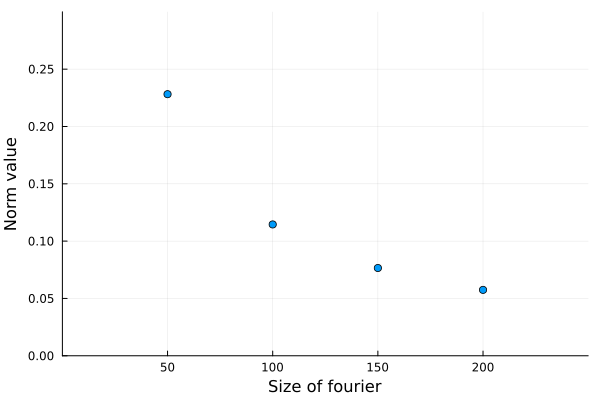
\includegraphics[scale=0.5]{img/scatter.png}
%DIFDELCMD <   \caption{フーリエ係数の次数の変更による$\|I_{X_2}\|$の比較}
%DIFDELCMD <   \label{fig:norm-gra}
%DIFDELCMD < \end{figure}
%DIFDELCMD < \end{comment}
%DIFDELCMD <  %%%
\DIFdelend \DIFaddbegin \begin{figure}[htbp]
  \centering
  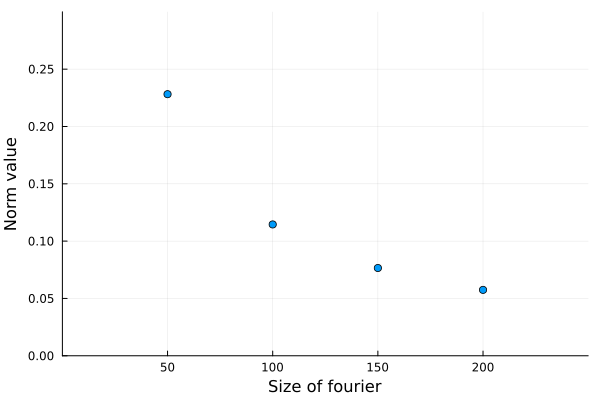
\includegraphics[scale=0.5]{img/scatter.png}
  \caption{\DIFaddFL{フーリエサイズとノルム値のグラフ}}
  \label{fig:norm-gra}
\end{figure}
 \DIFaddend \newpage 
 \newpage 
\chapter{おわりに}

本研究では,\rad{}を用いた精度保証付き数値計算の\DIFdelbegin \DIFdel{問題条件を緩和可能であるか検証するために,$l_1$空間}\DIFdelend \DIFaddbegin \DIFadd{問題適用範囲の拡大}\DIFaddend を\DIFdelbegin \DIFdel{用いたBanach空間上で,$DF(\bar{x})$が全単射であるかどうかを確かめた}\DIFdelend \DIFaddbegin \DIFadd{目的とした}\DIFaddend .\DIFdelbegin \DIFdel{$DF(\bar{x})$が全単射であるかを確かめるために}\DIFdelend \DIFaddbegin \DIFadd{\rad{}における作用素の計算に}\DIFaddend ,無限次元ガウスの消去法を用\DIFdelbegin \DIFdel{いた}\DIFdelend \DIFaddbegin \DIFadd{いることで,$l_\nu^1$を$l_1$と定義し,許容重みを定義に付加せずに解を導出できるかを検証した}\DIFaddend .プログラムによる検証により,\DIFdelbegin \DIFdel{$DF(\bar{x})$が全単射であることが確かめられた.この結果より,}\DIFdelend 無限次元ガウスの消去法を用いることで\DIFdelbegin \DIFdel{条件が緩和でき,}\DIFdelend \rad{}の精度の向上が可能であることがわかった.

今後の課題として,本研究では触れなかった評価値$Z_0, Z_1, Z_2(r)r$に対して,無限次元ガウスの消去法を用いて計算ができるか,また無限次元ガウスの消去法を用いた計算手法を導出することについて,検討をする.

\chapter*{謝辞}
本研究を進めるに際して, 千葉工業大学の関根晃太准教授には多くのご指導, ご助言を頂きました
こと深く感謝いたします。そして最後に、本研究に対しご助力頂いたすべての皆様に感謝し、お礼申し上げることで謝辞とさせて頂きます。
 \newpage 

\nocite{*}
%\bibliographystyle{junsrt}
%\bibliography{2131701}

%\begin{comment}
\begin{thebibliography}{99}
  \bibitem{b1} 大石進一, 精度保証付き数値計算, コロナ社 (2018)

  \bibitem{github}
  舩越康太, 井藤佳奈子, 大谷俊輔, 近藤慎佑, 高橋和暉, 瀬戸翔太, 二平泰知, 高安亮紀
  \newblock ``Julia 言語を使った精度保証付き数値計算のチュートリアル''
  \newblock \verb|https://github.com/tak-lab/rigorous_numerics_tutorial_julia,|,(2024/11/29)

  \bibitem{r1}関根晃太, 中尾充宏, 大石進一, Numerical verification methods for a system of elliptic PDEs,
  and their software library

  \bibitem{r2}  Kouta Sekine, Mitsuhiro T. Nakao, and Shin'ichi Oishi: “A new formulation using the Schur complement for the numerical existence proof of solutions to elliptic problems: without direct estimation for an inverse of the linearized operator”, Numer. Math., 146, 907–926, Oct., 2020.

\end{thebibliography}
%\end{comment}

 \newpage \begin{lstlisting}[caption=calc_solve.jl, label=calc_solve,]
  using LinearAlgebra, DifferentialEquations, FFTW
include("FourierChebyshev.jl")

# van der Pol方程式
function vanderpol(du, u, μ, t)
  x, y = u
  du[1] = y
  du[2] = μ * (1 - x^2) * y - x
end

# F^(N)(x_n)
function F_fourier(x, μ, η₀)
  N = length(x) / 2
  ω = x[1]
  a = x[2:end]
  (a³, ~) = powerconvfourier(a, 3)
  eta = sum(a) - η₀

  k = -(N - 1):(N-1)
  f = (-k .^ 2 * ω^2 - μ * im * k * ω .+ 1) .* a + μ * im * k * ω .* a³ / 3

  return [eta; f]
end

function DF_fourier(x, μ)
  N = Int((length(x)) / 2)
  ω = x[1]
  a = x[2:end]
  k = (-N+1):(N-1)
  (a³, ~) = powerconvfourier(a, 3)

  DF = zeros(ComplexF64, 2N, 2N)

  DF[1, 2:end] .= 1
  DF[2:end, 1] = (-2 * ω * k .^ 2 - μ * im * k) .* a + μ * im * k .* a³ / 3

  (~, a2) = powerconvfourier(a, 2)

  M = zeros(ComplexF64, 2 * N - 1, 2 * N - 1)

  for j = (-N+1):(N-1)
    M[k.+N, j+N] = μ * im * k * ω .* a2[k.-j.+(2*N-1)]
  end

  L = diagm(-k .^ 2 * ω^2 - μ * im * k * ω .+ 1)

  DF[2:end, 2:end] = L + M
  return DF
end

# a function of  fourier coeffs
function odefouriercoeffs(f, N, I, n=1)
  a = I[1]
  b = I[2]
  # x_j: equidistance node points
  h = (b - a) / (2N - 1)
  j = 0:2N-2
  xⱼ = a .+ j * h
  # f_j: function values on node points
  fⱼ = f(xⱼ)[n, :]
  return (fftshift(fft(fⱼ))) / (2 * N - 1)
end

# たぶん,初期値設定
u_0 = [0.0; 2.0]
tspan = (0.0, 300)
μ = 1.0
prob = ODEProblem(vanderpol, u_0, tspan, μ)
sol = solve(prob, Tsit5(), reltol=1e-8, abstol=1e-8)
u = hcat(sol.u...)
ind = floor(Int, length(sol.t) / 2)

# おおよその周期
#a = 30
#b = 36.55
a = 30
app_period = 6.55
timestep = 0.1

f_tmp = sol(a+app_period/2:timestep:a+3*app_period/2)
find_period = abs.(f_tmp .- sol(a))
(~, ind) = findmin(find_period[1, :])
b = a + app_period / 2 + timestep * (ind - 1)
#calc fouriercoeffs

N = 200 # size of Fourier

println("size of Fourier = $N")
a_0 = odefouriercoeffs(sol, N, [a, b])

include("IntervalFunctions.jl")
# Initial value of Newton method
η_0 = 0.0
x = [2 * pi / (b - a); a_0]

# Newton iteration
tol = 5e-12
F = F_fourier(x, μ, η_0)
println("Before step #1, ||F||_1 = $(norm(F,1))")
num_itr = 0

while num_itr ≤ 100
  global x = x - DF_fourier(x, μ) \ F
  global num_itr += 1
  global F = F_fourier(x, μ, η_0)
  # println("After step #$(num_itr), ||F||_1 = $(norm(F,1))")
  if norm(F, 1) < tol
    break
  end
end

# A^(N)
#ix = map(interval, x)
#iω̄ = map(interval, real(x[1]))
#iā = map(interval, x[2:end])

ix = x
iω̄ = real(x[1])
iā = x[2:end]

function DF_fourier(x::Vector{Complex{Interval{T}}}, μ) where {T}
  N = Int((length(x)) / 2)
  ω = x[1]
  a = x[2:end]
  k = (-N+1):(N-1)

  println("pcf Input: ", a, size(a), typeof(a))

  (a³, ~) = powerconvfourier(a, 3)
  DF = zeros(Complex{Interval{T}}, 2N, 2N)
  DF[1, 2:end] .= 1
  DF[2:end, 1] = (-2 * ω * k .^ 2 - μ * im * k) .* a + μ * im * k .* a³ / 3
  (~, a2) = powerconvfourier(a, 2)
  M = zeros(Complex{Interval{T}}, 2 * N - 1, 2 * N - 1)
  for j = (-N+1):(N-1)
    M[k.+N, j+N] = μ * im * k * ω .* a2[k.-j.+(2*N-1)]
  end
  L = diagm(-k .^ 2 * ω^2 - μ * im * k * ω .+ 1)
  DF[2:end, 2:end] = L + M
  return DF
end

iDF = DF_fourier(ix, μ);
iA = inv(iDF) # map(Interval,inv(mid.(iDF)))

## =======================
## I get a and omega by x.
## =======================
"""
println("x = $x")
println("μ = $μ")
println("N = $N")

μ
"""

omega = x[1]
a = x[2:end]
mu = μ

extend_size1 = (3 * N + 1)
extend_size2 = extend_size1 * 2 + 1
topleft_size = extend_size1

# define DF[]
zero_padding = zeros(ComplexF64, Int(extend_size2))
extend_x = vcat(omega, zero_padding, a, zero_padding)
extend_DF2 = DF_fourier(extend_x, mu)


# define A
zero_padding = zeros(ComplexF64, Int(extend_size1))
extend_x = vcat(omega, zero_padding, a, zero_padding)
extend_DF1 = DF_fourier(extend_x, mu)
T_inv = inv(extend_DF1)

## lambda 行列
topleft_size = size(T_inv)[1]
DF_bottomright = extend_DF2[topleft_size+1:end, topleft_size+1:end]
inv_lambda = inv(diagm(diag(DF_bottomright)))

# norm_D
D = inv_lambda * DF_bottomright
I_minus_D = 1.0I(size(D)[1]) - D
normI_minus_D = maximum(sum(abs.(I_minus_D), dims=1))

# norm_C
DF_bottomleft = extend_DF2[topleft_size+1:end, 1:topleft_size]
C = inv_lambda * DF_bottomleft
normC = maximum(sum(abs.(C), dims=1))

# norm_B
DF_topright = extend_DF2[1:topleft_size, topleft_size+1:end]
B = T_inv * DF_topright
normB = maximum(sum(abs.(B), dims=1))
normDF_topright = maximum(sum(abs.(DF_topright), dims=1))
normT_inv = maximum(sum(abs.(T_inv), dims=1))

println("||I - D|| = ", normI_minus_D)
println("||C|| = ", normC)
println("||T^-1|| = ", normT_inv)
println("||B|| = ", normB)

norm_result = normI_minus_D + normC * normT_inv * normB

println("||I - D|| + ||C|| ||T^-1|| ||B|| = ", norm_result)
\end{lstlisting}

\begin{lstlisting}[caption=FourierChebyshev.jl]
### Fourier functions
using FFTW, Plots
function fouriercoeffs(f, N, I=[0, 2π])
  # f: any periodic function on I
  # N: size of Fourier series
  a = I[1]
  b = I[2]
  h = (b - a) / (2N - 1)
  j = 0:2N-2
  xⱼ = a .+ j * h
  fⱼ = f.(xⱼ)
  return fftshift(fft(fⱼ)) / (2N - 1)
end

function odefouriercoeffs(f, N, I, n=1)
  a = I[1]
  b = I[2]
  h = (b - a) / (2N - 1)
  j = 0:2N-2
  xⱼ = a .+ j * h
  fⱼ = f(xⱼ)[n, :]
  return fftshift(fft(fⱼ)) / (2N - 1)
end

function plot_fourier(bc, I=[0, 2π])
  # bc: Fourier coefficients
  a = I[1]
  b = I[2]
  N = (length(bc) + 1) / 2 # 2N-1
  n_pad = 500
  bc_pad = [zeros(n_pad); bc; zeros(n_pad)]
  N_pad = N + n_pad
  h_pad = (b - a) / (2N_pad - 1)
  xj_pad = a .+ h_pad * (0:2N_pad-2)
  fNj_pad = real((2N_pad - 1) * ifft(ifftshift(bc_pad)))
  plot(xj_pad, fNj_pad, legend=false, xlabel="\$x\$", ylabel="\$f(x)\$")
end

function plot_fourier!(bc, I=[0, 2π]; label="")
  # bc: Fourier coefficients
  a = I[1]
  b = I[2]
  N = (length(bc) + 1) / 2 # 2N-1
  n_pad = 500
  bc_pad = [zeros(n_pad); bc; zeros(n_pad)]
  N_pad = N + n_pad
  h_pad = (b - a) / (2N_pad - 1)
  xj_pad = a .+ h_pad * (0:2N_pad-2)
  fNj_pad = real((2N_pad - 1) * ifft(ifftshift(bc_pad)))
  plot!(xj_pad, fNj_pad, label=label)
end

function plot_fouriercoeffs(bc)
  N = (length(bc) + 1) / 2 # 2N-1
  plot(-N+1:N-1, abs.(bc), yscale=:log10,
    legend=false,
    xlabel="\$k\$",
    ylabel="\$|\\bar{c}_k\\,|\$",
    title="Absolute values of Fourier coefficients"
  )
end

function plot_solution(u, index) # u = [ω, a_{-N+1}, ..., a_0, ..., a_{N-1}], length(u) = 2N
  # index = 1: profile of solution
  #         2: Fourier mode
  #         3: phase profile
  ω = real(u[1])
  L = 2π / ω
  a = u[2:end]
  N = length(u) / 2 # N: size of Fourier
  n_pad = 500
  a_pad = [zeros(n_pad); a; zeros(n_pad)]
  N_pad = N + n_pad
  dx = L / (2 * N_pad - 1)
  x = dx * (0:2*N_pad-2)
  if index == 1
    # Plot profile:
    plot(plot_fourier(a, [0, L]),
      # plot(x,real((2N_pad-1)*ifft(ifftshift(a_pad))),
      xlabel="\$t\$",
      ylabel="\$x\\,(t)\$",
      line=1.6,
      title="Profile of solution",
      size=(720, 400),
      legend=false,
    )
  elseif index == 2
    # Plot Fourier coefficients:
    plot(plot_fouriercoeffs(a),
      # plot((-N+1):(N-1),abs.(a),yscale=:log10,
      xlabel="\$k\$",
      ylabel="\$|a_k\\,|\$",
      line=1.6,
      title="Absolute values of Fourier coefficients",
      size=(720, 400),
      legend=false,
    )
  elseif index == 3
    # Plot phase:
    k = (-N_pad+1):(N_pad-1)
    plot(real((2N_pad - 1) * ifft(ifftshift(a_pad))), real((2N_pad - 1) * ifft(ifftshift(a_pad .* (im * k * ω)))),
      xlabel="\$x(t)\$",
      ylabel="\$\\dot{x}\\,(t)\$",
      line=1.6,
      title="Phase plot of a numerical solution",
      size=(720, 400),
      legend=false,
    )
  end
end

function plot_solution!(u)
  L = 2π / real(u[1])
  a = u[2:end]
  N = length(u) / 2
  n_pad = 1000
  a_pad = [zeros(n_pad); a; zeros(n_pad)]
  N_pad = N + n_pad
  k = (-N_pad+1):(N_pad-1)
  dx = L / (2 * N_pad - 1)
  x = dx * (0:2*N_pad-2)
  plot!(real((2N_pad - 1) * ifft(ifftshift(a_pad))), real((2N_pad - 1) * ifft(ifftshift(a_pad .* (im * k)))), line=1.6,)
end

function powerconvfourier(a::Vector{Complex{T}}, p) where {T}
  M = Int((length(a) + 1) / 2)
  N = (p - 1) * M
  ta = [zeros(N, 1); a; zeros(N, 1)] # 1. Padding zeros: size(ta) = 2pM-1
  tb = ifft(ifftshift(ta)) # 2. IFFT of ta
  tbᵖ = tb .^ p # 3. tb*^tb
  cᵖ = fftshift(fft(tbᵖ)) * (2.0 * p * M - 1)^(p - 1)
  return cᵖ[N+1:end-N], cᵖ[p:end-(p-1)]# return (truncated, full) version
end


### Chebyshev functions
function chebpts(n, a=-1, b=1) # n: order of Chebyshev polynomials
  m = -n:2:n
  x = sinpi.(m / (2 * n))
  return (1.0 .- x) .* a / 2 + (1.0 .+ x) .* b / 2
end

function chebcoeffs(f, M, I=[-1, 1])
  a = I[1]
  b = I[2]
  n = M - 1
  cpts = chebpts(n, a, b)
  fvals = f.(cpts)
  FourierCoeffs = real(fft([reverse(fvals); fvals[2:end-1]]))
  ChebCoeffs = FourierCoeffs[1:n+1] / n
  ChebCoeffs[1] = ChebCoeffs[1] / 2
  ChebCoeffs[end] = ChebCoeffs[end] / 2
  return ChebCoeffs # return Two-sided Chebyshev
end

function chebcoeffs_complex(f, M, I=[-1, 1])
  a = I[1]
  b = I[2]
  n = M - 1
  cpts = chebpts(n, a, b)
  fvals = f.(cpts)
  FourierCoeffs = fft([reverse(fvals); fvals[2:end-1]])
  ChebCoeffs = FourierCoeffs[1:n+1] / n
  ChebCoeffs[1] = ChebCoeffs[1] / 2
  ChebCoeffs[end] = ChebCoeffs[end] / 2
  return ChebCoeffs # return Two-sided Chebyshev
end

function cheb(f, I=[-1, 1]; tol=5e-15, Nmax=10000)
  a = I[1]
  b = I[2]
  m = 0.5 * (a + b)
  r = 0.5 * (b - a)
  x = rand(5)
  x1 = m .+ x * r
  x2 = m .- x * r
  if f.(x1) ≈ f.(x2)
    odd_even = 1 # even function: 1
  elseif f.(x1) ≈ -f.(x2)
    odd_even = -1 #  odd function: -1
  else
    odd_even = 0 # otherwise: 0
  end
  i = 3
  schbc = 0 # sampling chebyshev coefficients
  while true
    schbc = chebcoeffs(f, 2^i + 1, I)
    if all(abs.(schbc[end-2:end]) .< tol) || (2^i + 1 > Nmax)
      break
    end
    i += 1
  end
  M = findlast(abs.(schbc) .> tol)
  cc = schbc[1:M]
  # cc = chebcoeffs(f,M,I)
  if odd_even == 1 # even function
    cc[2:2:end] .= 0
  elseif odd_even == -1 # odd function
    cc[1:2:end] .= 0
  end
  return cc # return Two-sided Chebyshev
end

using GenericFFT
function bigcheb(f, I=[-1, 1]; tol=5e-15, Nmax=10000)
  a = I[1]
  b = I[2]
  m = 0.5 * (a + b)
  r = 0.5 * (b - a)
  x = rand(5)
  x1 = m .+ x * r
  x2 = m .- x * r
  if f.(x1) ≈ f.(x2)
    odd_even = 1 # even function: 1
  elseif f.(x1) ≈ -f.(x2)
    odd_even = -1 #  odd function: -1
  else
    odd_even = 0 # otherwise: 0
  end
  i = 3
  schbc = 0 # sampling chebyshev coefficients
  while true
    schbc = chebcoeffs(f, big(2^i + 1), I)
    if all(abs.(schbc[end-2:end]) .< tol) || (2^i + 1 > Nmax)
      break
    end
    i += 1
  end
  M = findlast(abs.(schbc) .> tol)
  cc = schbc[1:M]
  # cc = chebcoeffs(f,M,I)
  if odd_even == 1 # even function
    cc[2:2:end] .= 0
  elseif odd_even == -1 # odd function
    cc[1:2:end] .= 0
  end
  return cc # return Two-sided Chebyshev
end

function cheb_complex(f, I=[-1; 1]; tol=5e-15, Nmax=10000)
  i = 3
  schbc = 0 # sampling chebyshev coefficients
  while true
    schbc = chebcoeffs_complex(f, 2^i + 1, I)
    if all(abs.(schbc[end-2:end]) .< tol) || (2^i + 1 > Nmax)
      break
    end
    i += 1
  end
  M = findlast(abs.(schbc) .> tol)
  return schbc[1:M]
  # return cc # return Two-sided Chebyshev
end

function plot_chebcoeffs(f)
  zero_ind = findall(x -> x == 0, f)
  f[zero_ind] .= f[zero_ind.+1]
  plot(0:length(f)-1, abs.(f),
    yscale=:log10,
    title="Chebyshev coefficients",
    xlabel="Degree of Chebyshev polynomial",
    ylabel="Magnitude of coefficient",
    size=(800, 400),
    legend=false,
  )
end

function clenshaw(a, x) # Clenshaw's algorithm
  # a: (Two-sided) Chbyshev coefficients
  # x: evaluating points in [-1,1]
  n = length(a) - 1
  bk1 = 0.0
  bk2 = 0.0
  x = 2x
  for r = (n+1):-2:3
    bk2 = x .* bk1 .- bk2 .+ a[r]
    bk1 = x .* bk2 .- bk1 .+ a[r-1]
  end
  if isodd(n)
    b2 = x .* bk1 .- bk2 .+ a[2]
    bk2 = bk1 # b3
    bk1 = b2
  end
  return -bk2 .+ 0.5x .* bk1 .+ a[1] # y = c(1) + .5*x.*bk1 - bk2;
end

function clenshaw_secondkind(a, x) # Clenshaw's algorithm
  # a: (Two-sided) Chbyshev coefficients
  # x: evaluating points in [-1,1]
  n = length(a) - 1
  bk0 = 0
  bk1 = 0
  for r = (n+1):-1:1
    tmp = 2x .* bk0 .- bk1 .+ a[r]
    bk1 = bk0
    bk0 = tmp
  end
  return bk0 #.+ bk1*(-x)
end

function eval_cheb(a, x; I=[-1, 1])
  # a: (Two-sided) Chbyshev coefficients
  # x: evaluating points in domain
  ξ = 2 * (x .- I[1]) / (I[2] - I[1]) .- 1
  return clenshaw(a, ξ)
end

function eval_cheb_naive(ChebCoeffs_twosided, x; I=[-1, 1])
  M = length(ChebCoeffs_twosided) # M: size of chebyshev
  a = I[1]
  b = I[2]
  k = 0:M-1
  ξ = 2 * (x .- a) / (b - a) .- 1
  return cos.(Vector(k)' .* acos.(ξ)) * ChebCoeffs_twosided
end

function eval_cheb_bc(ChebCoeffs_twosided, x, n=200; I=[-1, 1]) # Barycentric interportion formula
  M = length(ChebCoeffs_twosided) # M: size of chebyshev
  a = I[1]
  b = I[2]
  k = 0:M-1
  ξⱼ = chebpts(n)
  xc = (1.0 .- ξⱼ) * a / 2 + (1.0 .+ ξⱼ) * b / 2 # Chebyshev points in [a,b]
  fxc = cos.(Vector(k)' .* acos.(ξⱼ)) * ChebCoeffs_twosided
  valnum = length(x)
  ξ = 2 * (x .- a) / (b - a) .- 1
  # ξ = range(-1,stop=1,length=valnum)
  # x = (1.0 .- ξ)*a/2 + (1.0 .+ ξ)*b/2
  λ = [1 / 2; ones(n - 1); 1 / 2] .* (-1) .^ (0:n)

  numer = zeros(valnum)
  denom = zeros(valnum)
  exact = zeros(Bool, valnum)

  for j = 1:n+1
    xdiff = x .- xc[j]
    temp = λ[j] ./ xdiff
    numer += temp * fxc[j]
    denom += temp
    exact[xdiff.==0] .= true
  end

  fx = numer ./ denom
  jj = findall(exact)
  fx[jj] = f.(x[jj])
  fx[jj] = cos.(Vector(k)' .* acos.(ξ[jj])) * ChebCoeffs_twosided
  return fx
end

function plot_cheb(ChebCoeffs_twosided; I=[-1, 1], title="", label="", legend=true) # Input: Two-sided Chebyshev
  # M = length(ChebCoeffs_twosided) # M: size of chebyshev
  # a = I[1]; b = I[2]; 
  x = range(I[1], stop=I[2], length=5000)
  # ξ = 2*(x.-a)/(b-a) .- 1
  fx = eval_cheb(ChebCoeffs_twosided, x, I=I)
  plot(x, fx, legend=legend, label=label, title=title, xlabel="\$x\$", ylabel="\$f(x)\$")
end

function plot_cheb!(ChebCoeffs_twosided; I=[-1, 1], title="", label="", legend=true) # Input: Two-sided Chebyshev
  # M = length(ChebCoeffs_twosided) # M: size of chebyshev
  # a = I[1]; b = I[2]; 
  x = range(I[1], stop=I[2], length=5000)
  # ξ = 2*(x.-a)/(b-a) .- 1
  fx = eval_cheb(ChebCoeffs_twosided, x, I=I)
  plot!(x, fx, legend=legend, label=label, title=title, xlabel="\$x\$", ylabel="\$f(x)\$")
end

function chebdiff(a; I=[-1, 1])# Input is Two-sided
  M = length(a)
  b = zeros(M + 1)
  for r = M-1:-1:1
    b[r] = b[r+2] + 2 * r * a[r+1]
  end
  b[1] /= 2.0
  return b[setdiff(1:end, end)] * (2 / (I[2] - I[1])) # Output is Two-sided
end

function chebdiff_oneside(a; I=[-1, 1])# Input is One-sided
  M = length(a)
  b = zeros(M + 1)
  for r = M-1:-1:1
    b[r] = b[r+2] + 2 * r * a[r+1]
  end
  return b[setdiff(1:end, end)] * (2 / (I[2] - I[1])) # Output is One-sided
end

function chebdiff_secondkind(a; I=[-1, 1])# Input is Two-sided
  M = length(a)
  b = zeros(M - 1)
  for n = 0:M-2
    b[n+1] = (n + 1) * a[n+2]
  end
  return b * (2 / (I[2] - I[1]))# Output is second kind (Two-sided)
end

function chebindefint(a; I=[-1, 1])# Input is Two-sided
  M = length(a)
  a_ext = zeros(M + 2)
  a_ext[1] = 2 * a[1]
  a_ext[2:M] = a[2:M]
  A = zeros(M + 1)
  for n = 1:M
    A[n+1] = (a_ext[n] - a_ext[n+2]) / (2n)
  end
  # A[1] = sum(A[2:2:end]) - sum(A[3:2:end]) # takes the value 0 at the left endpoint
  return A * (I[2] - I[1]) / 2
end

function chebint(a; I=[-1, 1])# Input is Two-sided
  M = length(a)
  n = 0:2:M-1
  return sum(2a[1:2:end] ./ (1.0 .- n .^ 2)) * ((I[2] - I[1]) / 2)
end

function chebroots(a, I=[-1, 1]) # Input is two-sided Chebyshev
  I_lo = I[1]
  I_up = I[2]
  n = length(a)
  # create colleague matrix
  du = [1; ones(n - 3) * 0.5]
  dl = ones(n - 2) * 0.5
  d = zeros(n - 1)
  A = Tridiagonal(dl, d, du)
  B = zeros(n - 1, n - 1)
  B[end, :] = a[1:end-1]
  C = A - (1 / (2 * a[n])) * B
  x = eigvals(C)
  ε = 100 * eps() * (I_up - I_lo) * 0.5
  if I_lo == -1.0 && I_up == 1.0
    return real(x[(-1-ε.≤real(x).≤1+ε).&(imag(x).≈0)])
  else
    x = real(x[(-1-ε.≤real(x).≤1+ε).&(imag(x).≈0)])
    return (1.0 .- x) .* I_lo / 2 + (1.0 .+ x) .* I_up / 2
  end
end

function endpoints_of_cheb(a) # Input is two-sided Chebyshev
  n = length(a)
  atm1 = dot((-1) .^ (0:n-1), a) # endpoint at -1
  at1 = sum(a) # endpoint at 1
  return atm1, at1
end

function chebmax(a, I=[-1, 1]) # Input is two-sided Chebyshev
  M = length(a)
  b = chebdiff(a)
  x = chebroots(b)
  fxc = eval_cheb(a, x)
  # k = 0:M-1
  # fxc = cos.((Vector(k))' .* acos.(x)) * a
  ep = endpoints_of_cheb(a)
  fvals = [ep[1]; fxc[1:end]; ep[2]]
  x = [interval(-1); x; interval(1)]
  ind = argmax(fvals)
  return x[ind], fvals[ind]
end

function chebmin(a, I=[-1, 1]) # Input is two-sided Chebyshev
  M = length(a)
  b = chebdiff(a)
  x = chebroots(b)
  fxc = eval_cheb(a, x)
  # k = 0:M-1
  # fxc = cos.((Vector(k))' .* acos.(x)) * a
  ep = endpoints_of_cheb(a)
  fvals = [ep[1]; fxc[1:end]; ep[2]]
  x = [interval(-1); x; interval(1)]
  ind = argmin(fvals)
  return x[ind], fvals[ind]
end
\end{lstlisting}


\DIFmodbegin
\begin{lstlisting}[caption=IntervalFunctions.jl,alsolanguage=DIFcode]
### Interval Matrix Multiplication
function ufp(P)
  u = 2.0^(-53)
  ϕ = 2.0^52 + 1
  q = ϕ * P
  T = (1 - u) * q
  return abs(q - T)
end

function succ(c)
  s_min = 2.0^-1074
  u = 2.0^-53
  ϕ = u * (1.0 + 2.0 * u)
  if abs(c) >= (1.0 / 2.0) * u^(-2) * s_min # 2^(-969)(Float64)
    e = ϕ * abs(c)
    succ = c + e
  elseif abs(c) < (1.0 / 2.0) * u^(-1) * s_min # 2^(-1022)(Float64)
    succ = c + s_min
  else
    C = u^(-1) * c
    e = ϕ * abs(C)
    succ = (C + e) * u
  end
  return succ
end

function pred(c)
  s_min = 2.0^-1074
  u = 2.0^-53
  ϕ = u * (1.0 + 2.0 * u)
  if abs(c) >= (1.0 / 2.0) * u^(-2) * s_min # 2^(-969)(Float64)
    e = ϕ * abs(c)
    pred = c - e
  elseif abs(c) < (1.0 / 2.0) * u^(-1) * s_min # 2^(-1022)(Float64)
    pred = c - s_min
  else
    C = u^(-1) * c
    e = ϕ * abs(C)
    pred = (C - e) * u
  end
  return pred
end

function mm_ufp(A_mid, B_mid) # A_mid, B_mid: Point matrix
  u = 2.0^(-53)
  realmin = 2.0^(-1022)
  n = size(A_mid, 2)

  if (2 * (n + 2) * u >= 1)
    error("mm_ufp is failed!(2(n+2)u>=1)")
  end
  # C_mid = A_mid * B_mid;
  # C_rad = (n+2) * u * ufp.(abs.(A_mid)*abs.(B_mid)) .+ realmin;
  # return C_mid, C_rad;
  return A_mid * B_mid, (n + 2) * u * ufp.(abs.(A_mid) * abs.(B_mid)) .+ realmin
end

function imm_ufp(A_mid, A_rad, B_mid, B_rad) # A = <A_mid, A_rad>, B = <B_mid, B_rad>: Interval matrix
  u = 2.0^(-53)
  realmin = 2.0^(-1022)
  n = size(A_mid, 2)

  if (2 * (n + 2) * u >= 1)
    error("mm_ufp is failed!(2(n+2)u>=1)")
  end
  #     C, R = mm_ufp(A_mid,B_mid);
  # C_mid = A_mid * B_mid;
  R = (n + 2) * u * ufp.(abs.(A_mid) * abs.(B_mid)) .+ realmin

  #     T_1, T_2 = mm_ufp(abs.(A_mid), B_rad);
  T1 = abs.(A_mid) * B_rad
  T2 = (n + 2) * u * ufp.(T1) .+ realmin

  #     T_3 = succ.(abs.(B_mid)+B_rad);
  T3 = succ.(abs.(B_mid) + B_rad)

  #     T_4, T_5 = mm_ufp(A_r, T_3);
  T4 = A_rad * T3
  T5 = (n + 2) * u * ufp.(T4) .+ realmin

  rad_sum = R + T1 + T2 + T4 + T5

  # C_rad = succ.(rad_sum + 4*u*ufp.(rad_sum));

  # return C_mid, C_rad;
  return A_mid * B_mid, succ.(rad_sum + 4 * u * ufp.(rad_sum))
end

# USE IntervalArithmetic.jl
using IntervalArithmetic
function int_mul(A::Matrix{T}, B::Matrix{T}) where {T}
  Cmid, Crad = mm_ufp(A, B)
  return interval(Cmid, Crad; format=:midpoint)
  # return Cmid .± Crad
end

function int_mul(A::Matrix{Interval{T}}, B::Matrix{T}) where {T}
  Cmid, Crad = imm_ufp(mid.(A), radius.(A), B, zeros(size(B)))
  return interval(Cmid, Crad; format=:midpoint)
  # return Cmid .± Crad
end

function int_mul(A::Matrix{T}, B::Matrix{Interval{T}}) where {T}
  Cmid, Crad = imm_ufp(A, zeros(size(A)), mid.(B), radius.(B))
  return interval(Cmid, Crad; format=:midpoint)
  # return Cmid .± Crad
end

function int_mul(A::Matrix{Interval{T}}, B::Matrix{Interval{T}}) where {T}
  Cmid, Crad = imm_ufp(mid.(A), radius.(A), mid.(B), radius.(B))
  return interval(Cmid, Crad; format=:midpoint)
  # return Cmid .± Crad
end

function int_mul(A::Matrix{Complex{T}}, B::Matrix{T}) where {T}
  Ar = real.(A)
  Ai = imag.(A) # (Ar + im*Ai)*B = Ar*B + im*(Ai*B)
  return complex.(int_mul(Ar, B), int_mul(Ar, B))
end

function int_mul(A::Matrix{T}, B::Matrix{Complex{T}}) where {T}
  Br = real.(B)
  Bi = imag.(B) # A*(Br + im*Bi) = A*Br + im*(A*Bi)
  return complex.(int_mul(A, Br), int_mul(A, Bi))
end

function int_mul(A::Matrix{Complex{T}}, B::Matrix{Complex{T}}) where {T}
  Ar = real.(A)
  Ai = imag.(A)
  Br = real.(B)
  Bi = imag.(B)
  # (Ar + im*Ai)*(Br + im*Bi) = (Ar*Br - Ai*Bi) + im*(Ar*Bi + Ai*Br)
  return complex.((int_mul(Ar, Br) - int_mul(Ai, Bi)), (int_mul(Ar, Bi) + int_mul(Ai, Br)))
end


### Interval Linear system solver
import LinearAlgebra: opnorm
function LinearAlgebra.opnorm(a::Matrix{Complex{Interval{Float64}}}, p::String)
  if p == "1"
    suma = sum(abs.(a), dims=1)
    return interval(maximum(inf, suma), maximum(sup, suma))
  elseif p == "Inf"
    suma = sum(abs.(a), dims=2)
    return interval(maximum(inf, suma), maximum(sup, suma))
  end
  return NaN
end

function LinearAlgebra.opnorm(a::Matrix{Interval{Float64}}, p::String)
  if p == "1"
    suma = sum(abs.(a), dims=1)
    return interval(maximum(inf, suma), maximum(sup, suma))
  elseif p == "Inf"
    suma = sum(abs.(a), dims=2)
    return interval(maximum(inf, suma), maximum(sup, suma))
  end
  return NaN
end

function verifylss_iB(iA, iB) # verify the solution element-wisely
  A = mid.(iA)
  B = mid.(iB)
  X̄ = A \ B
  n = size(X̄, 2)
  R = inv(A)
  #########
  iG = interval(Matrix{Float64}(I, n, n)) - interval(R) * iA
  α = opnorm(iG, "Inf")# Interval arithmetic
  #########
  if sup(α) < 1
    η = (abs.(iG) * interval(ones(n))) / (interval(1) - α)
    Err = interval(zeros(n, n))
    X̄ = interval(X̄)
    ir = iA * X̄ - iB # Interval arithmetic
    iRr = interval(R) * ir
    for i = 1:n
      Err[:, i] = abs.(iRr[:, i]) + interval(sup(norm(iRr[:, i], Inf))) * η # Interval arithmetic
    end
    return interval(X̄, Err, format=:midpoint)
  else
    println("Oh my way, verification is failed...")
    return nan
  end
end


### Interval all eigenvalues solver

function verifyalleig(iA, X)
  n = size(iA, 2)
  # iD = diagm(interval(λ))
  iX = interval(X)
  iB = int_mul(iA, iX)
  iG = verifylss_iB(iX, iB)
  ir = interval(zeros(n))
  ic = diag(iG)
  for i = 1:n
    for j = 1:n
      if i != j
        ir[i] += interval(mag(iG[i, j]))
      end
    end
    ir[i] += interval(radius(ic[i]))
  end
  return interval(ic, ir, format=:midpoint)
end

### Interval eigen solver (eigpair)

function verifyeig(iA::Matrix{Interval{T}}, lam, x, B=Matrix{T}(I, size(iA))) where {T<:Real}
  if typeof(lam) <: Complex || eltype(x) <: Complex
    lam = convert(Complex{T}, lam)
    x = convert.(Complex{T}, Vector(x))
  else
    lam = convert(T, lam)
    x = convert.(T, Vector(x))
  end
  x = x ./ norm(x)
  ysize = length(x)
  ilam = interval(lam)
  ix = interval(x)
  iB = interval(B)

  function iDF(w)
    mat = (zeros(typeof(ilam), length(w), length(w)))
    mat[1, 2:end] = transpose(interval(2) * (ix + w[2:end]))
    mat[2:end, 1] = -iB * (ix + w[2:end])
    mat[2:end, 2:end] = iA - (ilam + w[1]) * iB
    return mat
  end
  zero = zeros(T, ysize + 1)
  R = inv(mid.(iDF(zero)))
  iR = interval(R)
  iz = -iR * [dot(ix, ix) - interval(1.0); iA * ix - ilam * iB * ix]
  ϵ = 2 * sup(norm(iz, 1))
  if isreal(lam) && isreal(x)
    lam = real(lam)
    x = real(x)
    id = interval(0, ϵ; format=:midpoint)
    iy = interval.(zeros(ysize), ϵ; format=:midpoint)
    iI = interval(Matrix{T}(I, ysize + 1, ysize + 1))
  else
    id = Complex(interval(0, ϵ; format=:midpoint), interval(0, ϵ; format=:midpoint))
    iy = Complex.(interval.(zeros(ysize), ϵ; format=:midpoint), interval.(zeros(ysize), ϵ; format=:midpoint))
    iI = interval(Matrix{Complex{T}}(I, ysize + 1, ysize + 1))
  end
  iw = [id; iy]
  g(w) = iz + (iI - iR * iDF(w)) * w
  gw = g(iw)
  if all(issubset_interval.(gw, iw)) #gw .⊂ iw
    # while maximum(radius, gw) / norm([lam; x], 1) >= 1e3 * eps(T)
    #     gw = g(gw)
    # end
    return ilam + gw[1] #, ix .+ gw[2:end] #固有ベクトルも返すようにする
  else
    return NaN
  end
end

### Verify FFT using Interval Arithmetic
function verifyfft(z::Vector{Interval{T}}, sign=1) where {T}
  n = length(z)
  col = 1
  array1 = true
  if n == 1
    Z = map(T, z)
    return Z
  else
    isrow_ = false
  end
  log2n = Int(round(log2(n))) #check dimension
  if 2^log2n ≠ n # return error if n is not the powers of 2
    error("length must be power of 2")
  end
  #bit-reversal
  f = 2^(log2n - 1)
  v = [0; f]
  for k = 1:log2n-1
    f = f >> 1
    v = append!(v, f .+ v)
  end
  z2 = zeros(n, col)
  if isa(real(z[1]), Interval)
    z2 = map(T, z2)
  end
  # replace z
  for j = 1:n
    z2[j, :] = z[v[j]+1, :]
  end
  #Danielson-Lanczos algorithm
  Z = complex(map(Interval, z2))
  Index = reshape([1:n*col;], n, col)

  theta = map(Interval, sign * (0:n-1) / n) # division exact because n is power of 2
  itheta = map(interval, theta)
  Phi = cospi.(itheta) + im * sinpi.(itheta) # SLOW?
  # Phi = cospi.(theta) + im*sinpi.(theta)

  v = [1:2:n;]
  w = [2:2:n;]
  t = Z[w, :]
  Z[w, :] = Z[v, :] - t
  Z[v, :] = Z[v, :] + t
  for index in 1:(log2n-1)
    m = 2^index
    m2 = 2 * m
    vw = reshape([1:n;], m2, Int(n / m2))
    v = vw[1:m, :]
    w = vw[m+1:m2, :]
    indexv = reshape(Index[v[:], :], m, Int(col * n / m2))
    indexw = reshape(Index[w[:], :], m, Int(col * n / m2))
    Phi1 = repeat(Phi[1:Int(n / m):end], outer=[1, Int(col * n / m2)])
    t = Phi1 .* Z[indexw]
    Z[indexw] = Z[indexv] - t
    Z[indexv] = Z[indexv] + t
  end
  reverse(Z[2:end, :], dims=2)
  if sign == -1
    Z = Z / n
  end
  if isrow_
%    Z = transpose(Z)#transpose of Z
  end
  if array1
    Z = Z[:, 1]
  end
  return Z
end

### Rigorous convolution algorithm via FFT
function powerconvfourier(ia::Vector{Complex{Interval{T}}}, p) where {T}
  M = Int((length(ia) + 1) / 2) # length(a) = 2M-1
  N = (p - 1) * M

  length_ia = 2 * p * M - 1
  length_ia_ext = nextpow(2, length_ia)# 2pM-2+2L

  L = Int((length_ia_ext - length_ia + 1) / 2)

  # step.1 : padding (p-1)M + L zeros for each sides
  ia_ext = map(Complex{Interval}, zeros(length_ia_ext))
  ia_ext[L+N+1:end-L-N+1] = ia  #\tilda{a}

  # step.2 : inverse fft
  ib_ext = verifyfft(ifftshift(ia_ext), -1) #sign = -1 : ifft

  # step.3 : power p elementwisely
  ib_extᵖ = ib_ext .^ p

  # step.4 : fft with rescaling
  ic_extᵖ = fftshift(verifyfft(ib_extᵖ, 1)) * length_ia_ext^(p - 1)  #sign = 1 : fft

  #     return ic_extᵖ,ic_extᵖ
  return ic_extᵖ[L+N+1:end-N-L+1], ic_extᵖ[L+p:end-(L+p-2)] # return (truncated, full) version
end

function convfourier(ia...)
  p = length(ia)
  M = Int((length(ia[1]) + 1) / 2) # length(a) = 2M-1
  N = (p - 1) * M

  length_ia = 2 * p * M - 1
  length_ia_ext = nextpow(2, length_ia)# 2pM-2+2L

  # itbᵖ = ones(Interval,N+length(ia[1])+N)
  # ibp_ext = map(Complex{Interval},ones(length_ia_ext))
  ibp_ext = interval(ones(ComplexF64, length_ia_ext))

  L = Int((length_ia_ext - length_ia + 1) / 2)

  for i = 1:p
    # step.1 : padding (p-1)M + L zeros for each sides
    # ia_ext = map(Complex{Interval},zeros(length_ia_ext))
    ia_ext = interval(zeros(ComplexF64, length_ia_ext))
    @show length(ia[i])
    @show length(ia_ext[L+N+1:end-L-N+1])
    @show length(ia[i])
    ia_ext[L+N+1:end-L-N+1] = ia[i]  #\tilda{a}
    # step.2 : inverse fft
    ib_ext = verifyfft(ifftshift(ia_ext), -1) #sign = -1 : ifft
    # step.3 : power p elementwisely
    ibp_ext = ibp_ext .* ib_ext
    # ib_extᵖ = ibp_ext.^p
  end
  # step.4 : fft with rescaling
  ic_extᵖ = fftshift(verifyfft(ibp_ext, 1)) * length_ia_ext^(p - 1)  #sign = 1 : fft
  return ic_extᵖ[L+N+1:end-N-L+1], ic_extᵖ[L+p:end-(L+p-2)] # return (truncated, full) version
end

function convcos(ia...) # Input: Two-sided (real)
  M = length(ia[1])
  FourierCoeffs = []
  for i = 1:length(ia)
    ia[i][1] = ia[i][1]
    ia[i][2:end] = 0.5 * ia[i][2:end] # Two-sided -> One-sided (real)
    FC_local = map(Complex, [reverse(ia[i][2:end]); ia[i]])
    if i == 1
      FourierCoeffs = tuple(FC_local)
    else
      FourierCoeffs = tuple(FourierCoeffs..., tuple(FC_local)...)
    end
  end
  icp, icp_full = convfourier(FourierCoeffs...) # real -> complex (input)
  iap = interval(zeros(M))
  iap[1] = real(icp[M])
  iap[2:end] = 2 * real(icp[M+1:end]) # One-sided (complex) -> Two-sided (real)
  N = Int((length(icp_full) + 1) / 2) #2N-1
  iap_full = interval(zeros(N))
  iap_full[1] = real(icp_full[N])
  iap_full[2:end] = 2 * real(icp_full[N+1:end]) # One-sided (complex) -> Two-sided (real)
  return iap, iap_full
end
\end{lstlisting}
\DIFmodend
 \newpage 

%% 定義 dfn
%% 定理 thm
%% 証明 proof
%% 補題 lmm

%---------------

%%文章のあとに,\cite{label1, label2},\cite{lite:xxx}とつける
%隙間ができたら,\newlineを入れ込む
%% rpa = radii polynomial approach

\end{document}
